%/**********************************************************************/
%		第5章:CAMベース超並列SIMD型プロセッサアーキテクチャ
%/**********************************************************************/
\chapter{CAMベース超並列SIMD型\mbox{プロセッシングアーキテクチャ}}
\label{lbl_chptr5}

本章では,マルチメディアデータ処理におけるテーブルルックアップ処理と
繰り返し演算処理の高速化を両立する,新しいメモリベースのマルチメディアLSI
アーキテクチャを提案する.
テーブルルックアップ処理は,\ref{lbl_chptr3}章,及び\ref{lbl_chptr4}章にて
示したCAMベースのテーブルルックアップ符号化アーキテクチャを利用する.
繰り返し演算の高速な処理については,SRAMをベースとして,
演算器の配置とデータの処理ベクトルを工夫することにより
並列度を大幅に向上させることを実現した超並列SIMD型演算プロセッサを
新たに開発した.
本章では,上記2つのメモリベースアーキテクチャを融合することで,
プログラマブルに様々なマルチメディアアプリケーションの高速な処理を可能としながら,
小面積,低消費電力である,CAMベース超並列SIMD型プロセッサ
のアーキテクチャを提案し,その性能評価について述べる.

本章の構成は,\ref{lbl_cp5_intro}節において,CAMベース超並列SIMD型プロセッサの
基本概念について述べる.
\ref{lbl_cp5_mta}節では,繰り返し演算処理を高速に処理することが可能な
SRAMベース超並列SIMD型プロセッサについて詳述し,
\ref{lbl_cp5_mtb}節において,CAMベースのテーブルルックアップ符号化アーキテクチャ
との融合について論じるとともに,CAMベース超並列SIMD型プロセッサについて詳述する.
\ref{lbl_cp5_jpg}節では,提案アーキテクチャをJPEGアプリケーションに適用した場合の
性能を評価し,\ref{lbl_cp5_matome}節にて,本章のまとめを述べる.



\subsection{動作概要}
\label{lbl_cp5_mta_simd_prc}

超並列SIMD型プロセッサは,SRAM領域から演算器にデータを送り込むことによって四則演算等の
処理を行うことが可能である.以下に加算,減算,乗算,及び除算の例を示す.
尚,図中に示すXはテンポラリレジスタ,CBはキャリーを格納するレジスタ,Mはマスクレジスタである.
加算の例を図 \ref{mta_add},減算の例を図 \ref{mta_sub1},図 \ref{mta_sub2},乗算の例を図 \ref{mta_mul1},図 \ref{mta_mul2},及び除算の例を
図 \ref{mta_div1},図 \ref{mta_div2},図 \ref{mta_div3}に示す.

%figure
	\begin{figure}[tbh]
		\begin{center}
			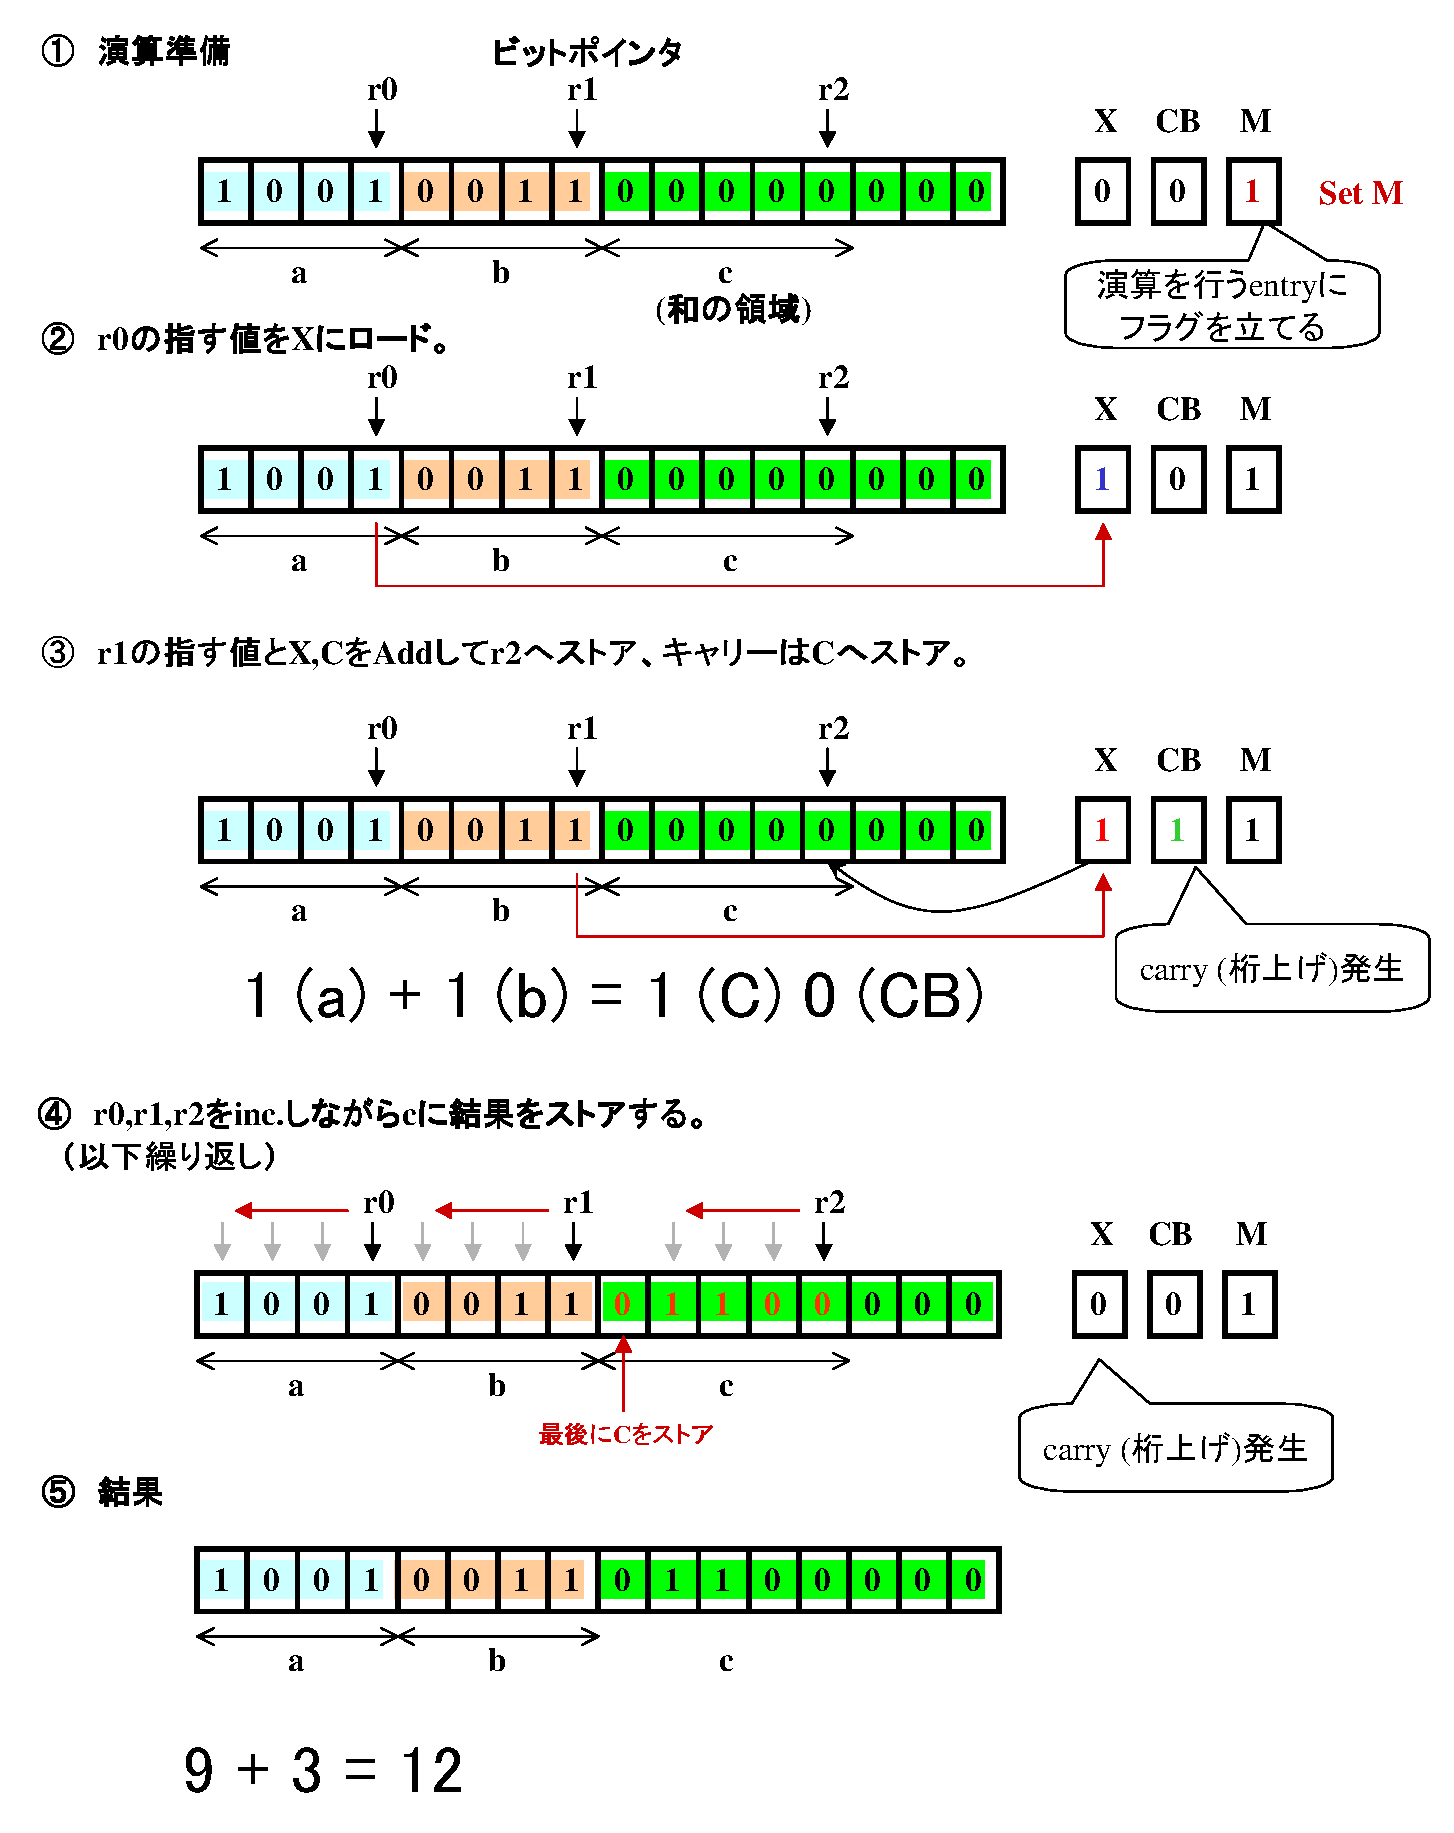
\includegraphics[width = 14cm,  height = 14cm, keepaspectratio, clip]{./pics/mta_add.eps}
		\end{center}
		\caption{超並列SIMD型プロセッサの加算処理.}
%		\ecaption{FMCAM with $d$ bits $\times$ $2^a$ words.}
		\label{mta_add}
	\end{figure}%	
%figure	

%figure
	\begin{figure}[tbh]
		\begin{center}
			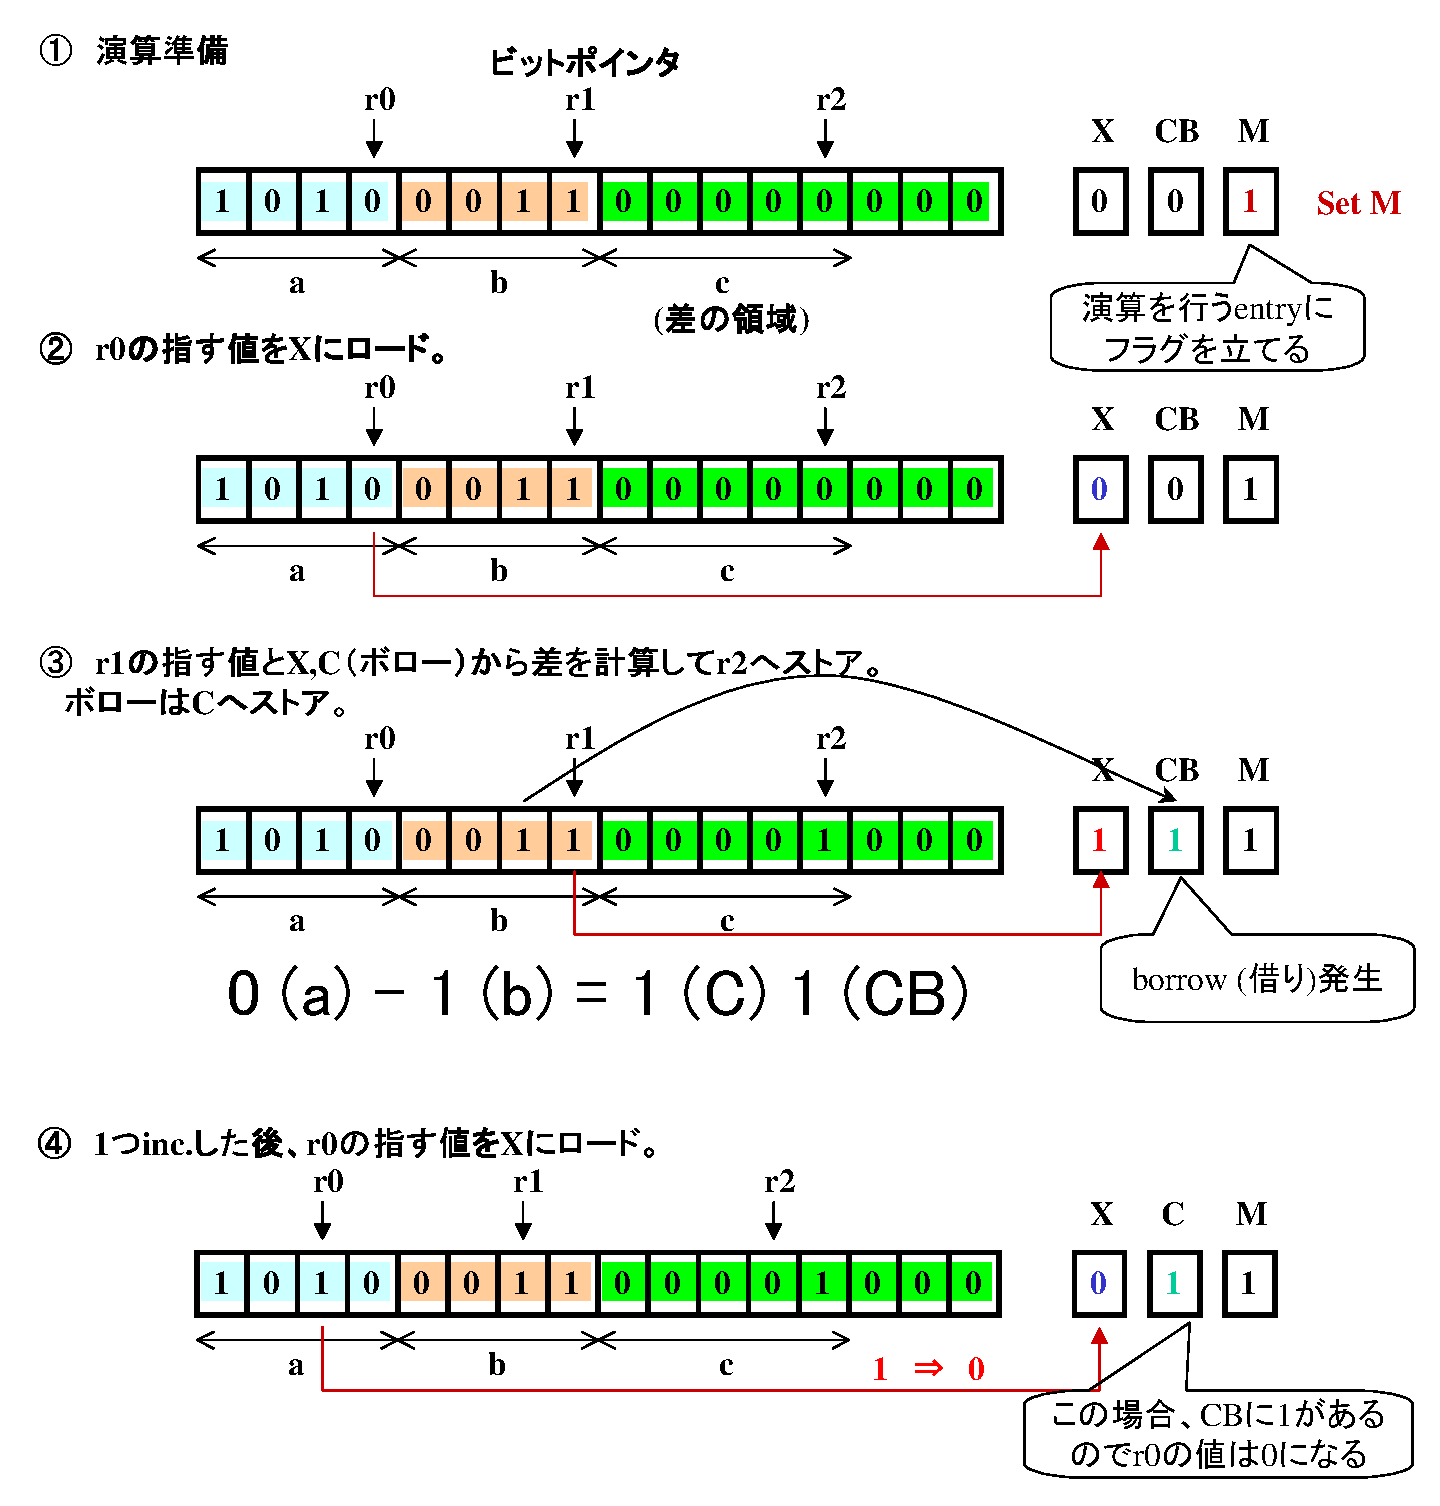
\includegraphics[width = 14cm,  height = 14cm, keepaspectratio, clip]{./pics/mta_sub1.eps}
		\end{center}
		\caption{超並列SIMD型プロセッサの減算処理 (1/2).}
%		\ecaption{FMCAM with $d$ bits $\times$ $2^a$ words.}
		\label{mta_sub1}
	\end{figure}%	
%figure	

%figure
	\begin{figure}[tbh]
		\begin{center}
			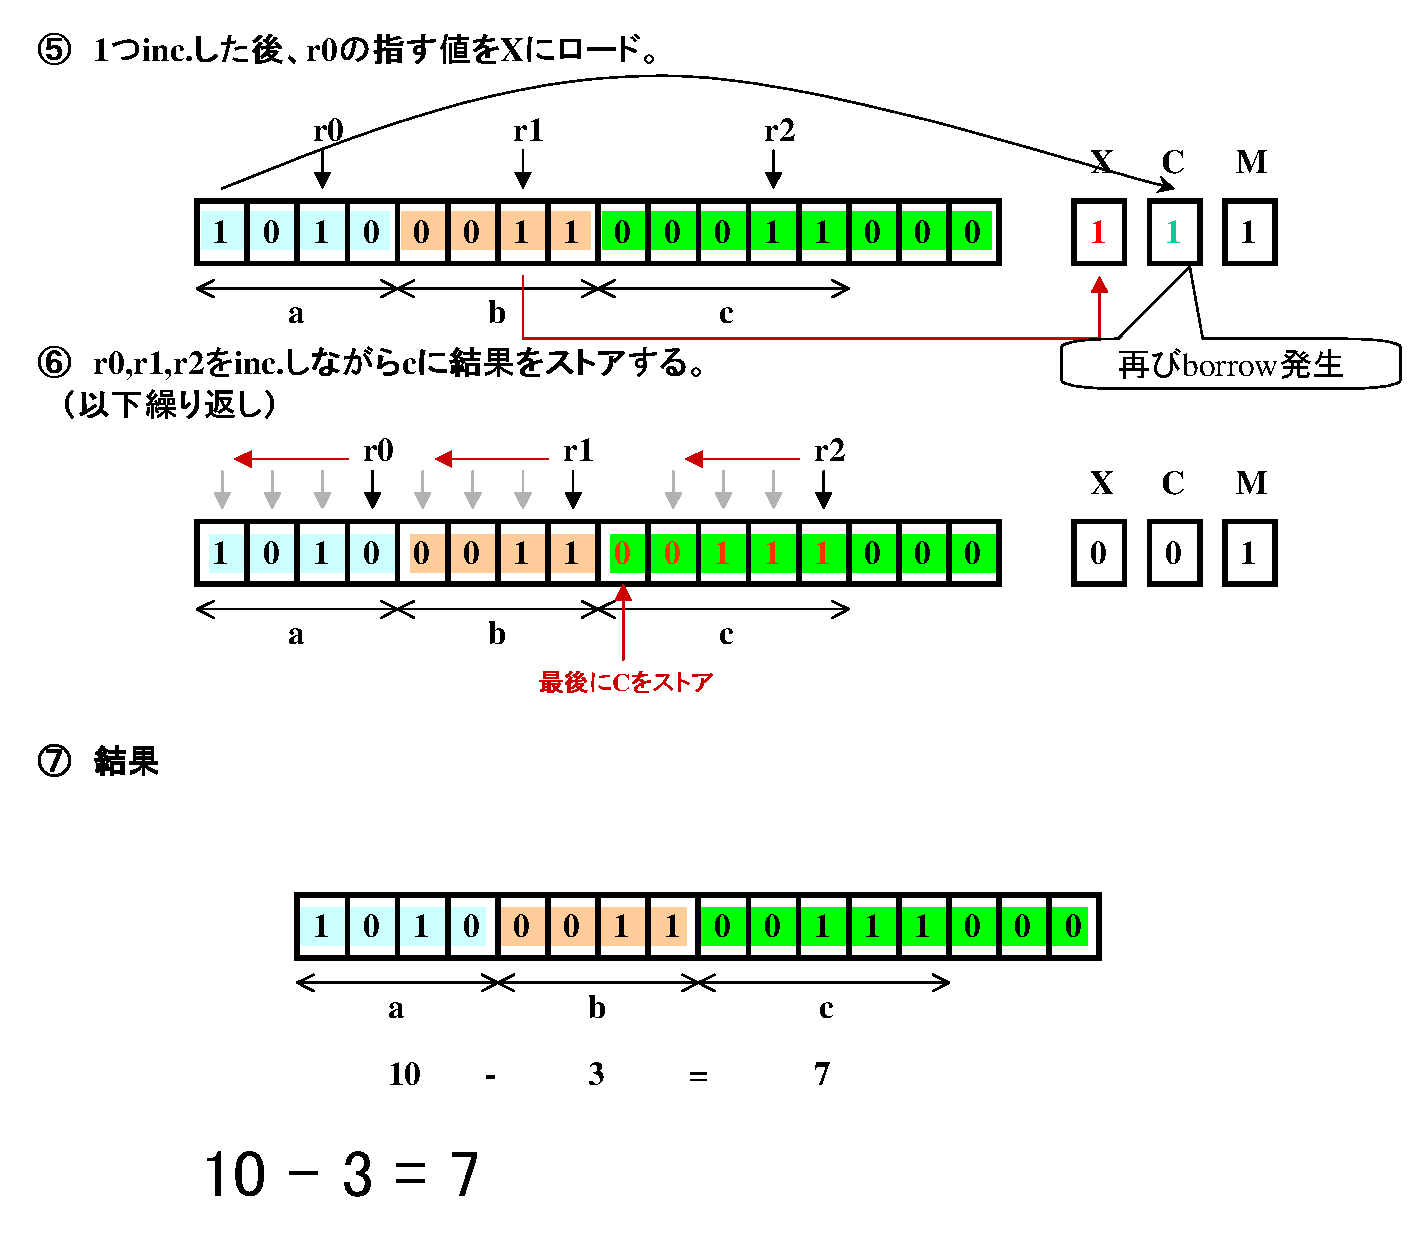
\includegraphics[width = 14cm,  height = 14cm, keepaspectratio, clip]{./pics/mta_sub2.eps}
		\end{center}
		\caption{超並列SIMD型プロセッサの減算処理 (2/2).}
%		\ecaption{FMCAM with $d$ bits $\times$ $2^a$ words.}
		\label{mta_sub2}
	\end{figure}%	
%figure	

%figure
	\begin{figure}[tbh]
		\begin{center}
			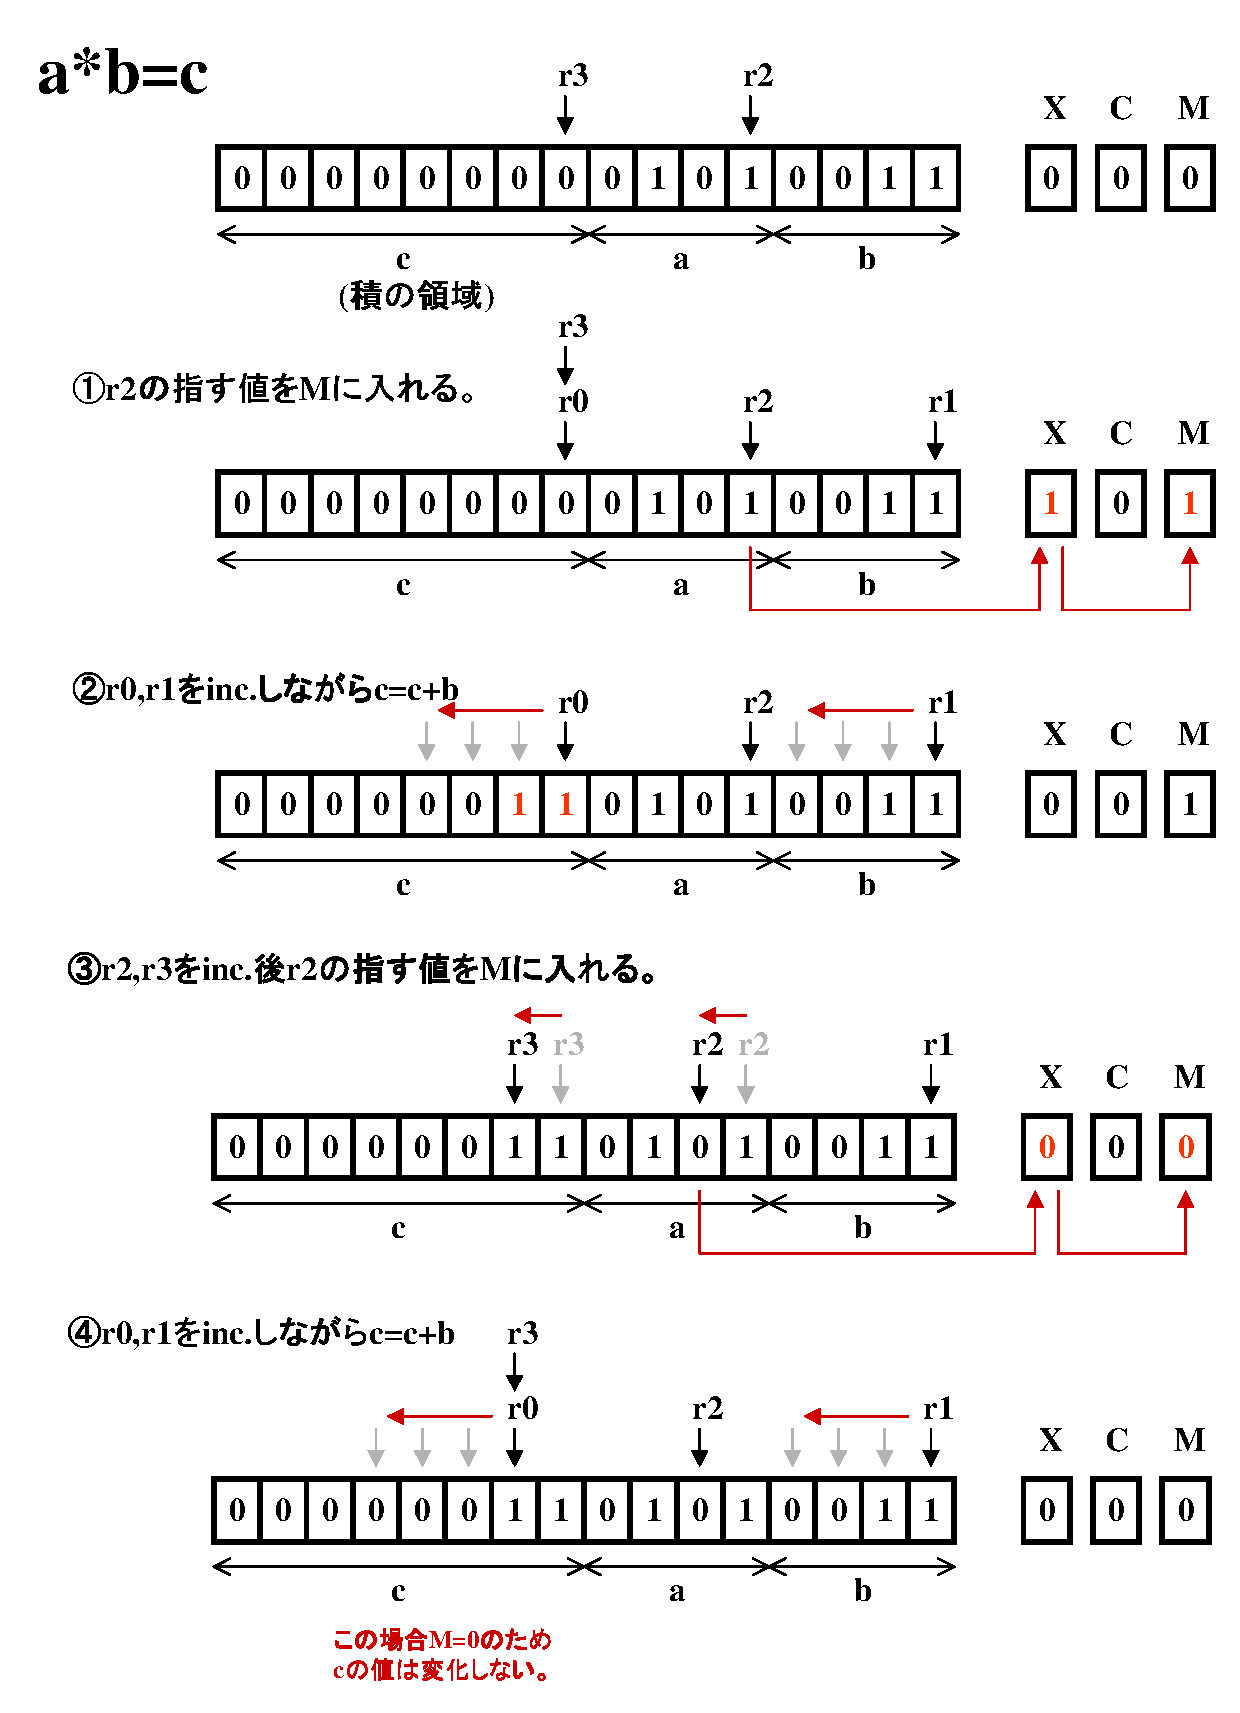
\includegraphics[width = 14cm,  height = 14cm, keepaspectratio, clip]{./pics/mta_mul1.eps}
		\end{center}
		\caption{超並列SIMD型プロセッサの乗算処理 (1/2).}
%		\ecaption{FMCAM with $d$ bits $\times$ $2^a$ words.}
		\label{mta_mul1}
	\end{figure}%	
%figure	

%figure
	\begin{figure}[tbh]
		\begin{center}
			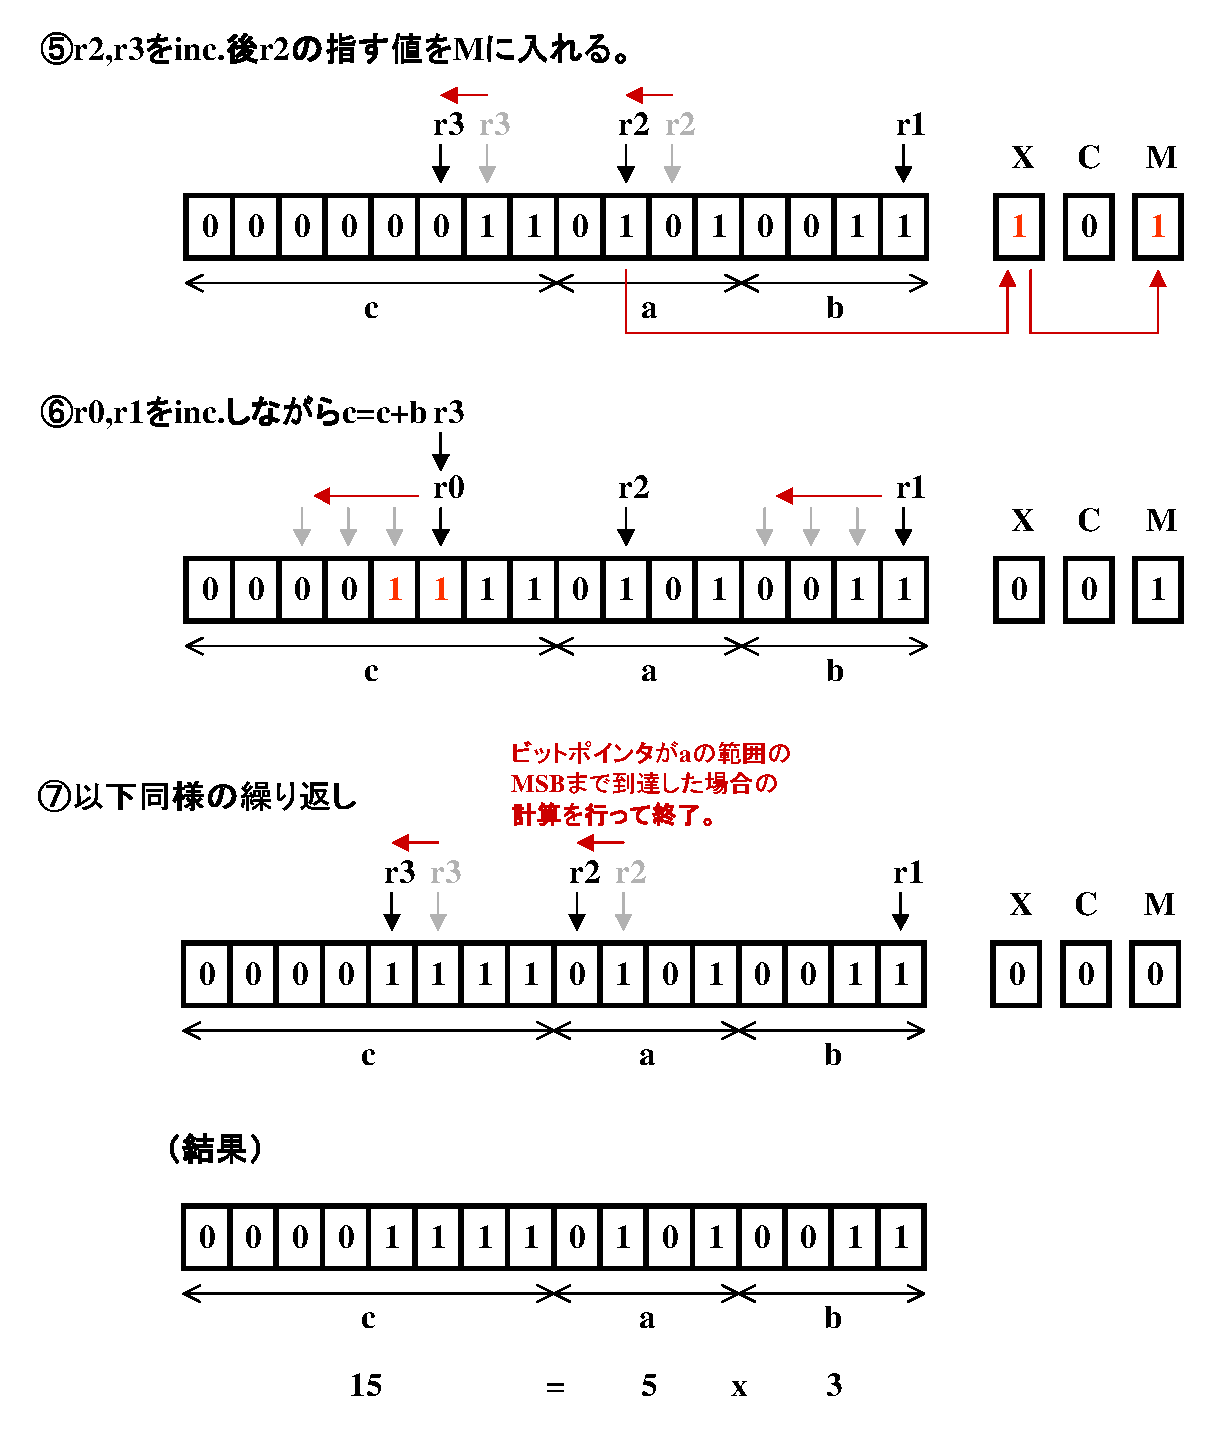
\includegraphics[width = 14cm,  height = 14cm, keepaspectratio, clip]{./pics/mta_mul2.eps}
		\end{center}
		\caption{超並列SIMD型プロセッサの乗算処理 (2/2).}
%		\ecaption{FMCAM with $d$ bits $\times$ $2^a$ words.}
		\label{mta_mul2}
	\end{figure}%	
%figure	

%figure
	\begin{figure}[tbh]
		\begin{center}
			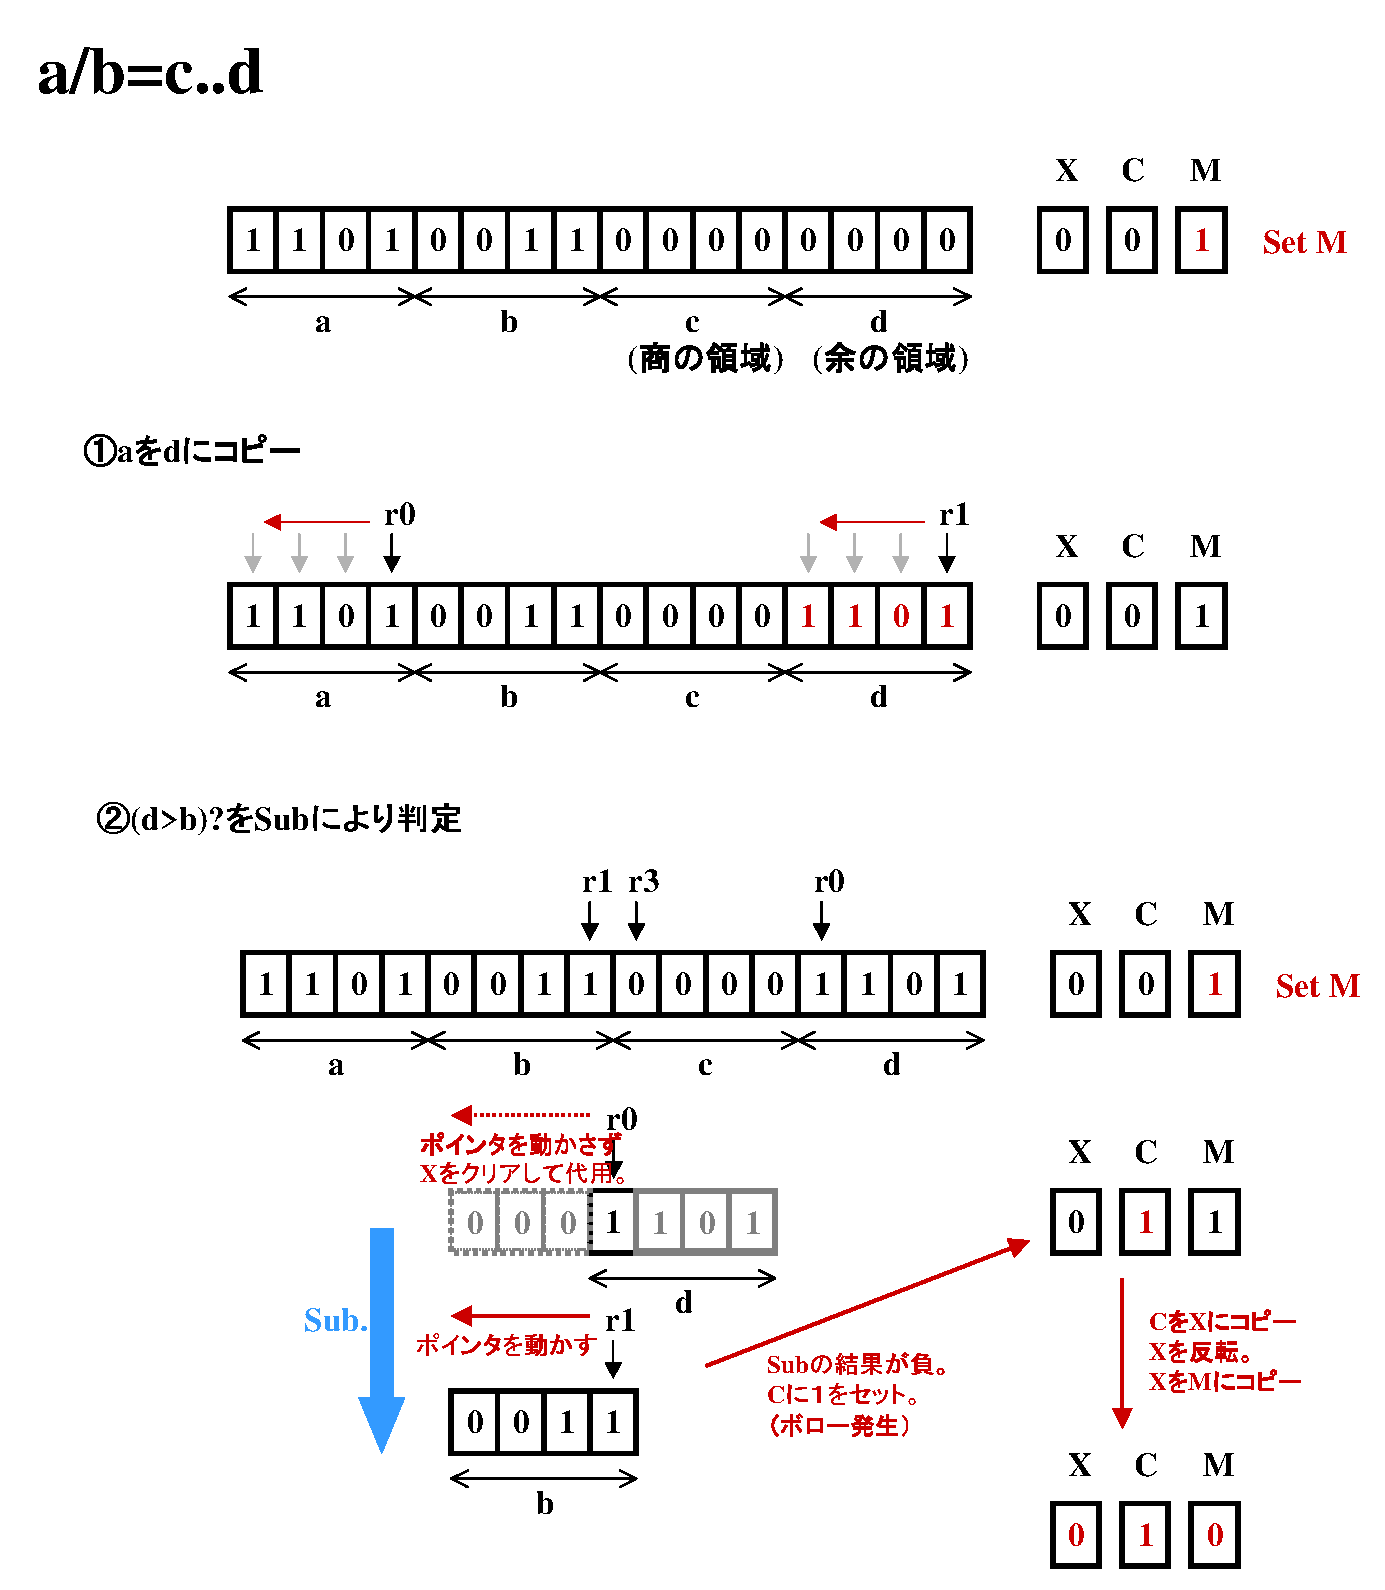
\includegraphics[width = 14cm,  height = 14cm, keepaspectratio, clip]{./pics/mta_div1.eps}
		\end{center}
		\caption{超並列SIMD型プロセッサの除算処理 (1/3).}
%		\ecaption{FMCAM with $d$ bits $\times$ $2^a$ words.}
		\label{mta_div1}
	\end{figure}%	
%figure	

%figure
	\begin{figure}[tbh]
		\begin{center}
			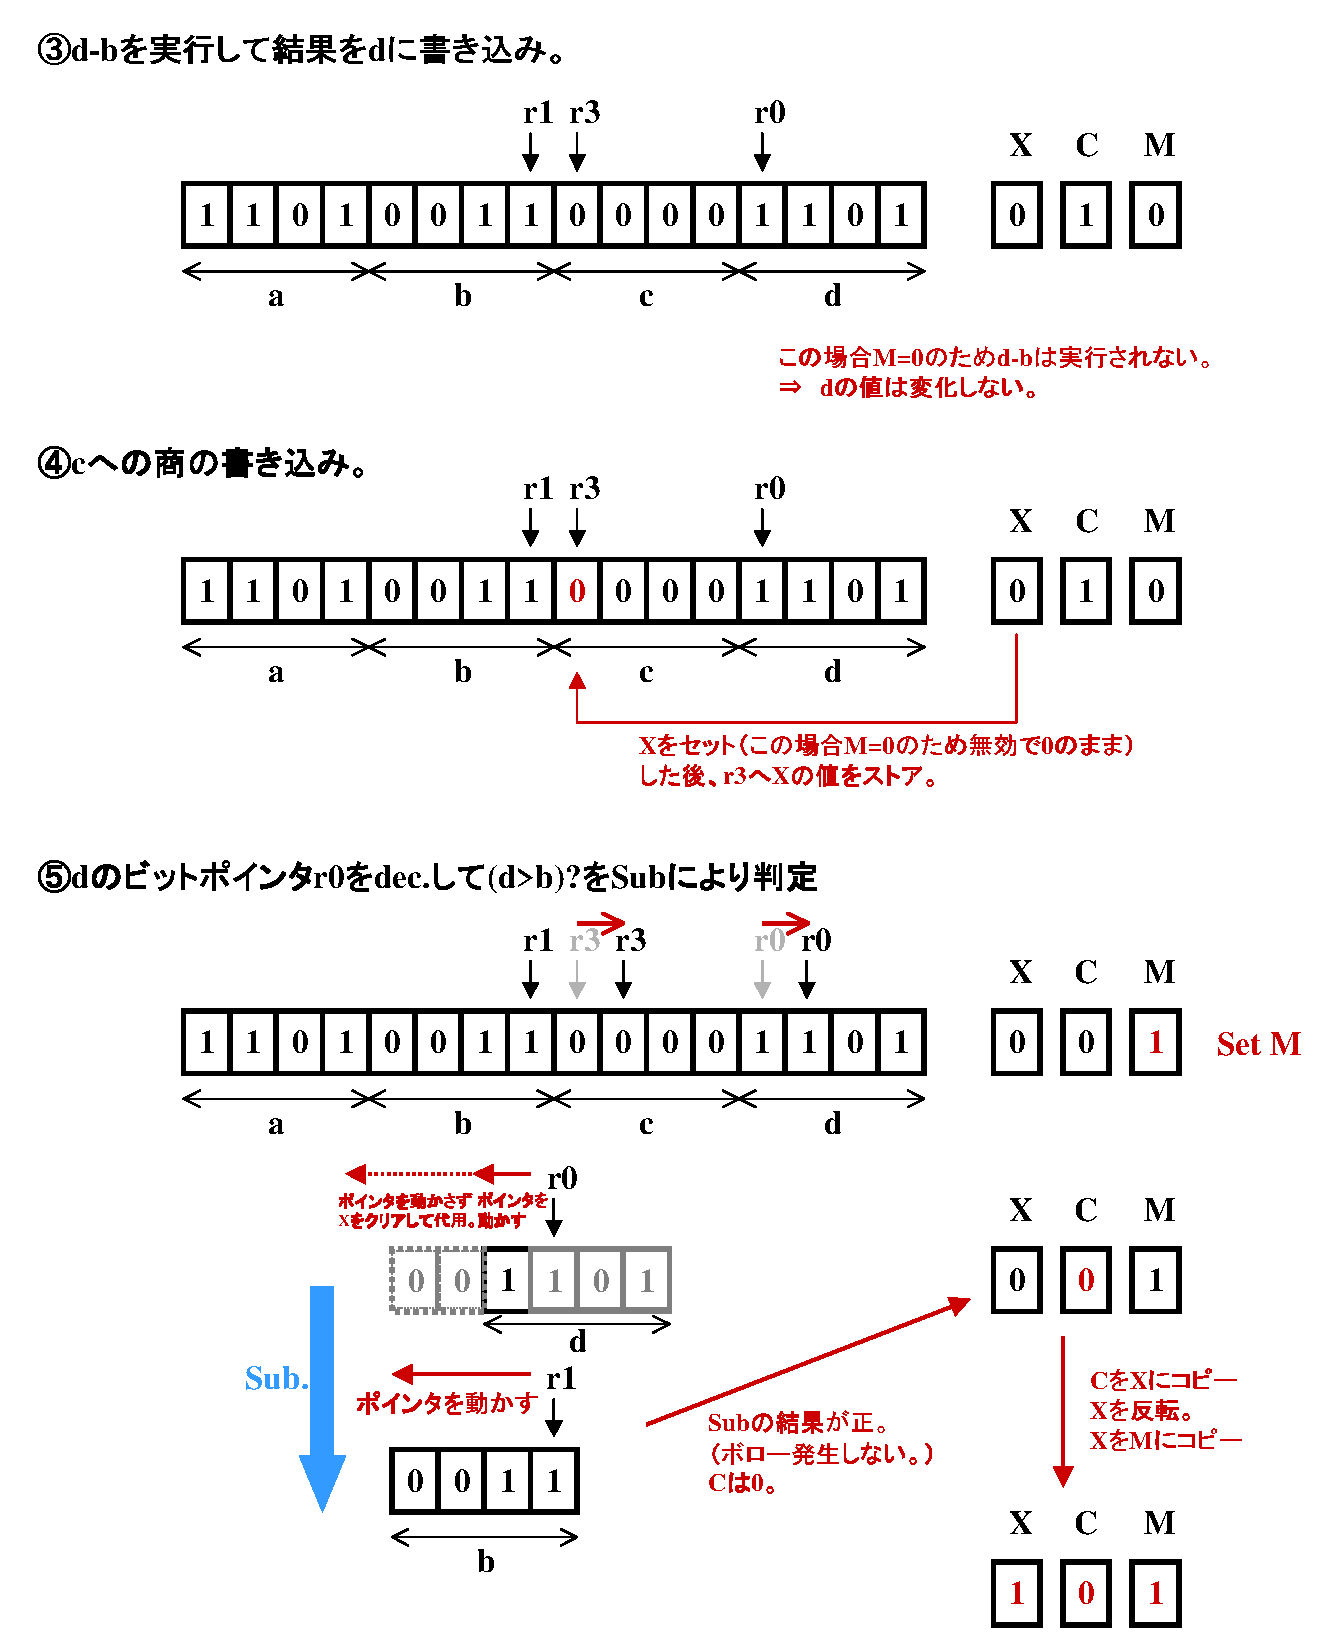
\includegraphics[width = 14cm,  height = 14cm, keepaspectratio, clip]{./pics/mta_div2.eps}
		\end{center}
		\caption{超並列SIMD型プロセッサの除算処理 (2/3).}
%		\ecaption{FMCAM with $d$ bits $\times$ $2^a$ words.}
		\label{mta_div2}
	\end{figure}%	
%figure	

%figure
	\begin{figure}[tbh]
		\begin{center}
			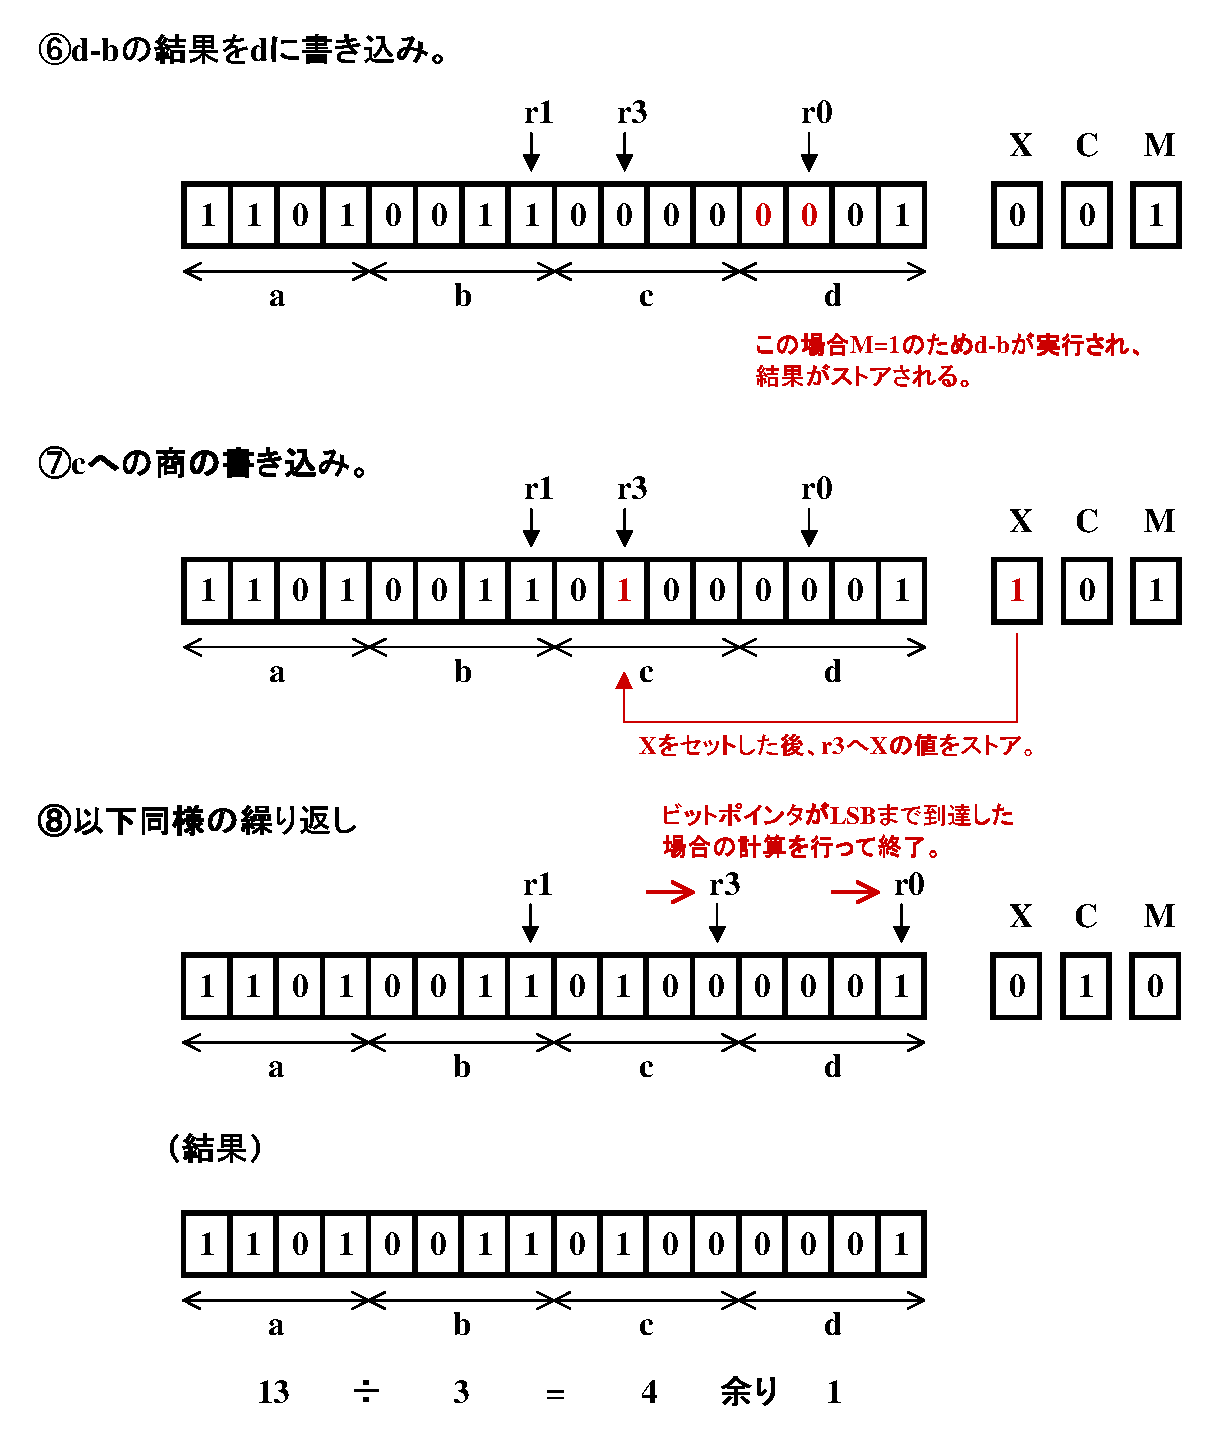
\includegraphics[width = 14cm,  height = 14cm, keepaspectratio, clip]{./pics/mta_div3.eps}
		\end{center}
		\caption{超並列SIMD型プロセッサの除算処理 (3/3).}
%		\ecaption{FMCAM with $d$ bits $\times$ $2^a$ words.}
		\label{mta_div3}
	\end{figure}%	
%figure	

\clearpage

\subsection{VLSI設計結果}
\label{lbl_cp5_mta_simd_impl}

超並列SIMD型プロセッサを,90 nm CMOS技術によって共同開発した\cite{mppnnd06}.
開発結果を表 \ref{mta_impl}に,チップ写真を図 \ref{mta_pics}に示す.
チップの概要は,2,048並列の演算器と,500 Kbit (256 bit,2,048 entry)のSRAMを2面
備えている.実装面積は3.1 mm$^2$であり,1.2 V時に200 MHzで動作する.
消費電力は1.2 V時,250 mWであり,モバイル機器向けの数値としては
十分低いものであるといえる.
また,演算能力は16 bitの加算を行った場合,40 GOPSという高い値を示した.


%figure*
	\begin{table}[thb]
	\centering
		\begin{center}
		\caption{90 nm CMOS技術による,超並列SIMD型プロセッサの実装結果.}
%			\includegraphics[width = 8.5cm, height = 8.5cm, keepaspectratio, clip]{impl_rslt.eps}
			\includegraphics[width = 12cm, height = 12cm, keepaspectratio, clip]{./pics/mta_impl.eps}
		\label{mta_impl}
		\end{center}
	\end{table}%
%figure*


%figure
	\begin{figure}[tbh]
		\begin{center}
			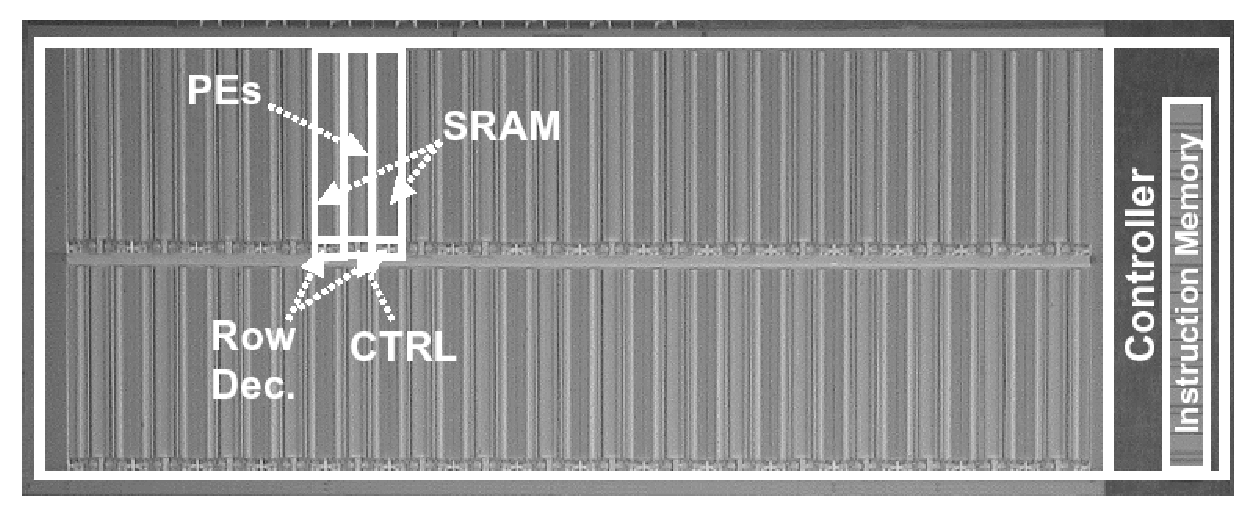
\includegraphics[width = 14cm,  height = 14cm, keepaspectratio, clip]{./pics/mta_pics.eps}
		\end{center}
		\caption{超並列SIMD型プロセッサのチップ写真.}
%		\ecaption{FMCAM with $d$ bits $\times$ $2^a$ words.}
		\label{mta_pics}
	\end{figure}%	
%figure	


\section{CAMと超並列SIMD型プロセッシングアーキテクチャの融合}
\label{lbl_cp5_mtb}

	マルチメディアデータ処理の主要なボトルネックとなっていたテーブルルックアップ処理については,
	\ref{lbl_chptr3}章,及び\ref{lbl_chptr4}章にて,CAMベースのテーブルルックアップ符号化を適用することで
	高速かつ高圧縮に処理ができることを示した.
	もう一方の処理である繰り返し演算は\ref{lbl_cp5_mta}節にて,SRAMベースの
	超並列SIMD型プロセッサアーキテクチャによって高速に処理できることを示した.
	この章では,上記2つのアーキテクチャを融合させて,マルチメディアアプリケーションを
	高速,高圧縮かつプログラマブルに処理することのできる,新規性の高い
	高性能なCAMベースの超並列SIMD型プロセッサアーキテクチャについて述べる.

\subsection{融合処理の概要}
\label{lbl_cp5_mtb_idea}

CAMベーステーブルルックアップ符号化アーキテクチャと
SRAMベース超並列SIMD型プロセッサアーキテクチャを融合するためには,
まず,各アーキテクチャのデータ処理手法の違いに着目しなければならない.
図 \ref{op_mthd}に示しているように,CAMベーステーブルルックアップ符号化アーキテクチャの
テーブルルックアップ処理は図 \ref{op_mthd}-(A)の処理であり,
超並列SIMD型プロセッサアーキテクチャによる繰り返し演算は,図 \ref{op_mthd}-(B)の処理となるからである.
そのため,両アーキテクチャが相互にデータをやり取りし,協調動作をするためには,
マルチメディアデータの直交変換を行うインタフェースモジュールを中心に
両アーキテクチャで挟み込む形にすることが,データ転送の際の消費電力や,配線長に伴う
面積及び配線遅延の削減の面で効果的であると考えられる.
インタフェースモジュールとSRAMベース超並列SIMD型アーキテクチャの配置については,
図 \ref{mta_intf}で示した構成を用いる.CAMベーステーブルルックアップ符号化アーキテクチャの融合に関しては,
以下に求められる機能と,使用可能なメモリアーキテクチャについて述べた後,構成を決定する.

CAMベーステーブルルックアップ符号化アーキテクチャの融合に関して求められる機能は,以下の通りである.

\begin{enumerate}
\item CPUバスから送信されるデータを直交変換し,SIMD型演算モジュールに転送する機能
\item SIMD型演算モジュールから出力されるデータを直交変換し,CPUバスに送信する機能
\item CPUバスから送信されるデータを処理し,再度CPUバスへ送信する機能
\item SIMD型演算モジュールから出力されるデータを処理し,再度SIMD型演算モジュールに出力する機能
\item SIMD型演算モジュールのボトルネックであるテーブルルックアップ処理を行う機能
\item SIMD型演算モジュールのボトルネックである一致検索処理を行う機能
\item 汎用性
\item 小面積及び低消費電力
\end{enumerate}

これらの求められる機能を実現するために必要な処理は,大きく分けて
データの直交変換を行う処理と,入力データと同一のデータを符号化テーブルから一致検索する処理である.
そのため融合化には,以下に示すメモリアーキテクチャを組み合わせて実現する方法が考えられる.

\begin{enumerate}
\item Static Random Access Memory (SRAM)

入力ポート及び出力ポートを一対もつメモリであり,データの書き込み及び読み出しが可能である.

\item 直交SRAM

水平方向の入力ポート及び出力ポートを一対,垂直方向の入力ポート,及び出力ポートを一対もつ
メモリである.
ブロック図は図 \ref{hv_sram}に示してある.
SRAM同様データの書込み,及び読み出しが可能である.
また,水平方向から入力されるデータを垂直方向に出力する,もしくは垂直方向から入力されるデータを
水平方向に出力することによってデータの直交変換を可能にすることができる.
ただし,直交変換処理を行った場合,数十ビットのワード単位で入力されるデータは,
1 bitづつ出力されることとなる.

\item Content Addressable Memory (CAM)

通常の読み書きを行うことのできるメモリに,特定の機能を付加した機能メモリの一種であり,
内部に格納されているデータと入力されるデータとの間で一致検索処理を行うことのできるものである.
データを格納しているメモリセルの付近に比較器を配置することで,検索処理を実現する構成をとっており,
通常この一致検索処理にかかる時間は,他のソフトウェア及びハードウェアより高速である.

\item 直交CAM

直交SRAM,及びCAM両方の機能を有する機能メモリである.
ブロック図を図 \ref{hv_cam}に示す.

%figure
	\begin{figure}[tbh]
		\begin{center}
			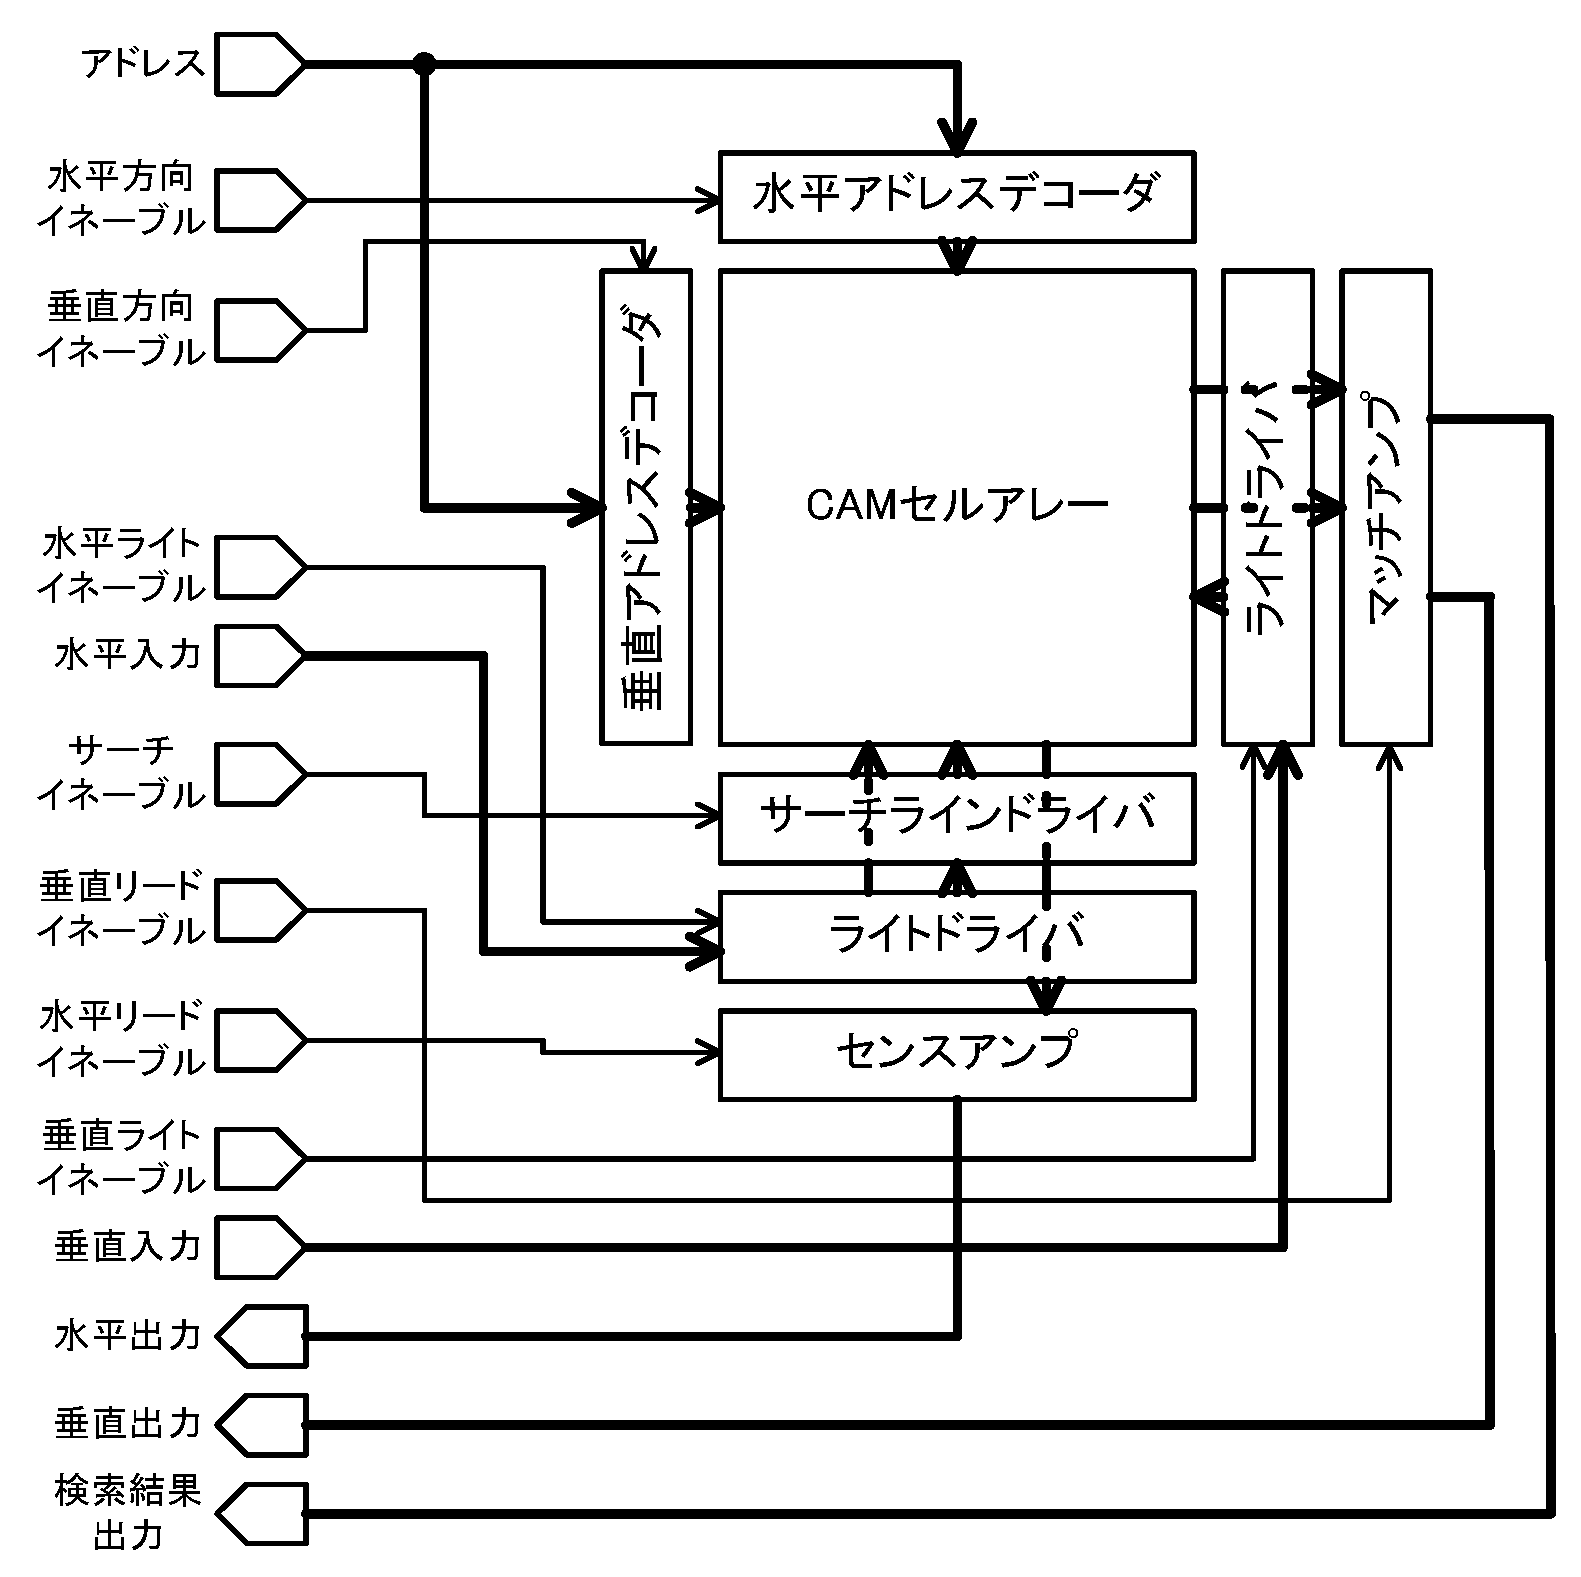
\includegraphics[width = 12cm,  height = 12cm, keepaspectratio, clip]{./pics/hv_cam.eps}
		\end{center}
		\caption{直交CAMのブロック図.}
%		\ecaption{FMCAM with $d$ bits $\times$ $2^a$ words.}
		\label{hv_cam}
	\end{figure}%	
%figure	

\end{enumerate}

融合の際には,これらのメモリアーキテクチャを組み合わせて,前述した機能の充足度を
評価したうえで,テーブルルックアップインタフェースモジュールを実装することとなる.
表 \ref{mtb_an}に,検討したメモリアーキテクチャの組み合わせを示す.
各組み合わせ案については,インターリーブを動作とテーブルルックアップの両立を踏まえつつ,
冗長度が少ないものを選出してある.
これらの組み合わせ案を元に,各機能の実現を評価した結果を,
表 \ref{mtb_an_hyoka}に示す.
各項目A (高性能に実現可能),B (実現可能),及びC (実現は困難)の3段階で評価した.
ただし,面積の見積もりに関しては組み合わせ1の実装面積を3として,各組み合わせ案の
面積を算出している.
検討の結果,機能の実現性,将来性,及び実装面積等で最も有効なのは
CAMを直交SRAMの近傍に配置した構成をとる組み合わせ3の案となった.

%figure*
	\begin{table}[thb]
	\centering
		\begin{center}
		\caption{テーブルルックアップモジュール構築のためのメモリモジュール組み合わせ案.}
%			\includegraphics[width = 8.5cm, height = 8.5cm, keepaspectratio, clip]{impl_rslt.eps}
			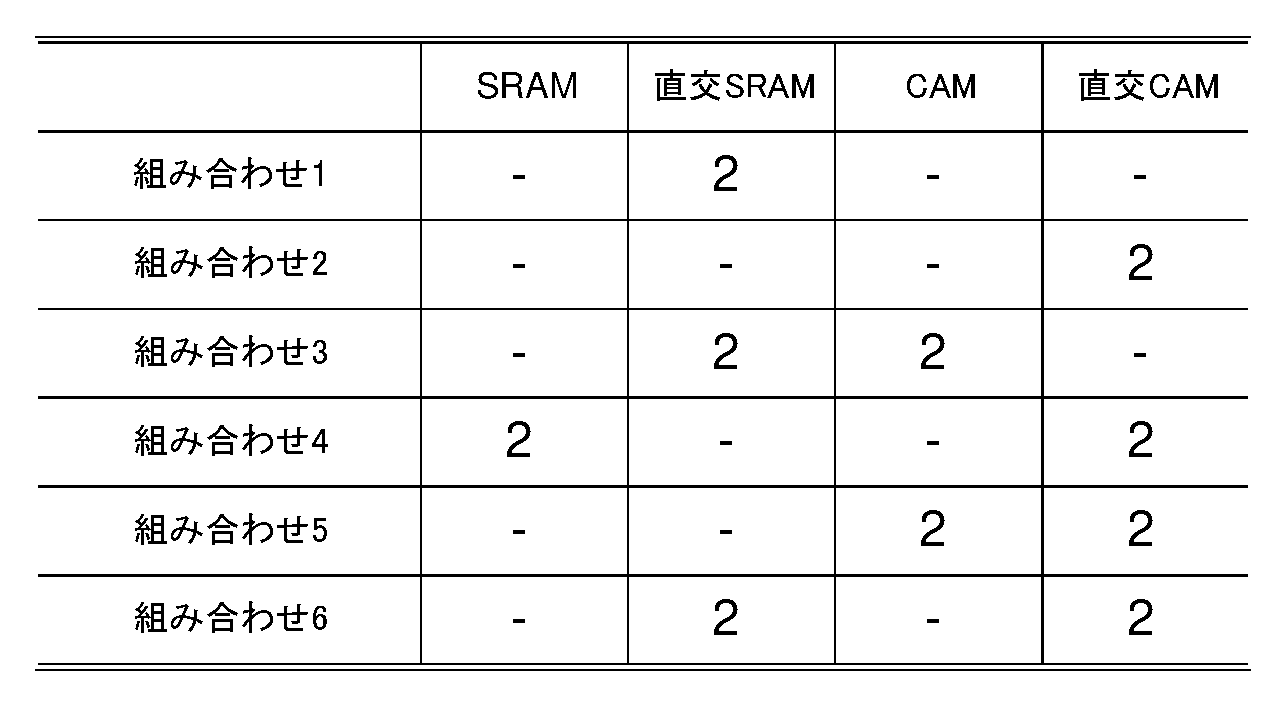
\includegraphics[width = 12cm, height = 12cm, keepaspectratio, clip]{./pics/mtb_an.eps}
		\label{mtb_an}
		\end{center}
	\end{table}%
%figure*

%figure*
	\begin{table}[thb]
	\centering
		\begin{center}
		\caption{メモリモジュール組み合わせ案に対する機能実現の評価結果.}
%			\includegraphics[width = 8.5cm, height = 8.5cm, keepaspectratio, clip]{impl_rslt.eps}
			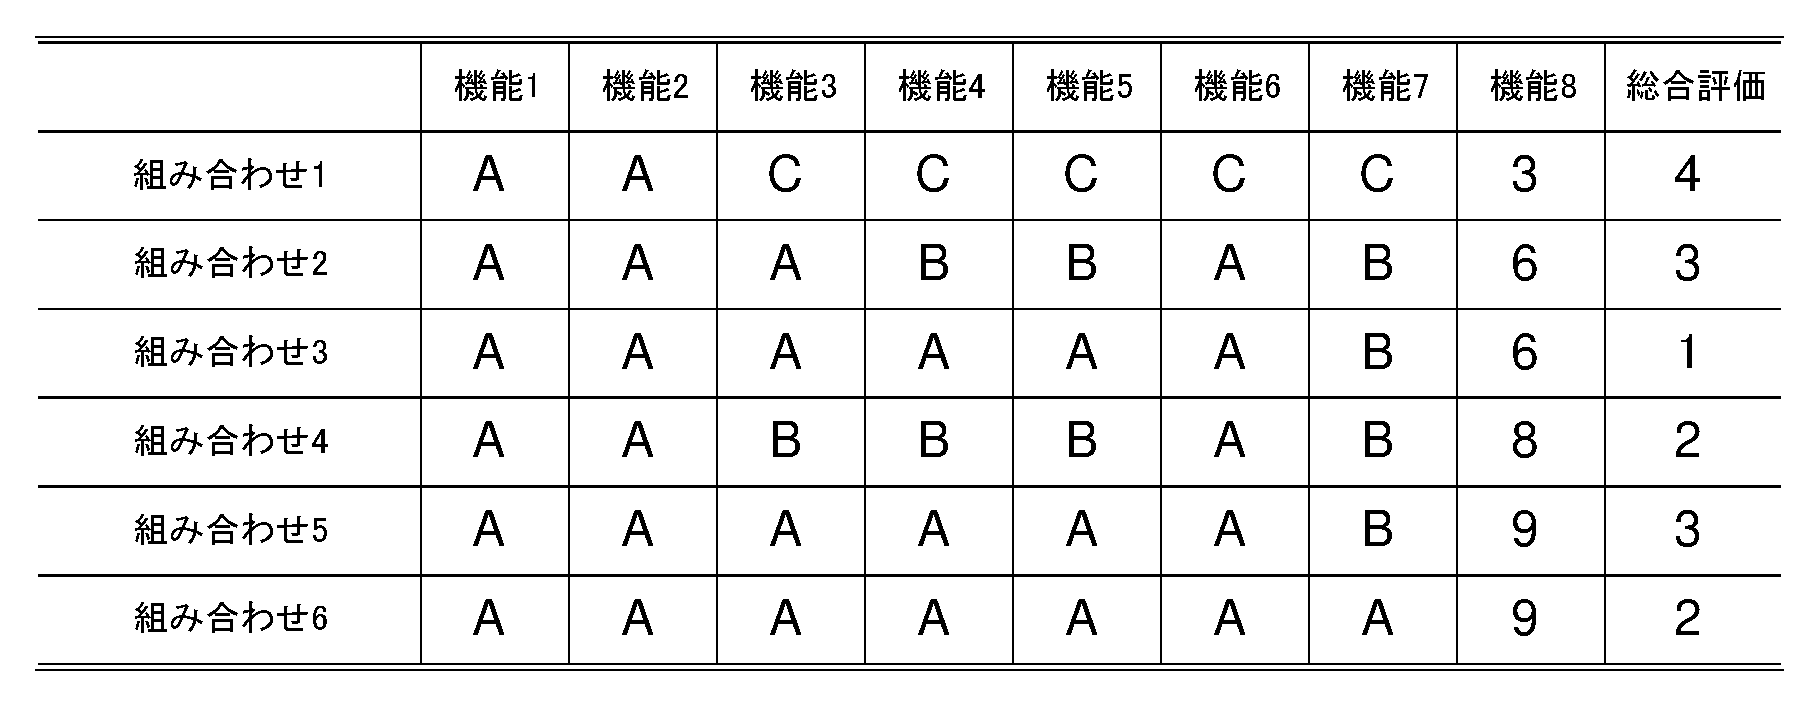
\includegraphics[width = 14cm, height = 14cm, keepaspectratio, clip]{./pics/mtb_an_hyoka.eps}
		\label{mtb_an_hyoka}
		\end{center}
	\end{table}%
%figure*

\clearpage

\subsection{アーキテクチャ}
\label{lbl_cp5_mtb_arch}

\ref{lbl_cp5_mtb_idea}節の検討結果より,マルチメディアデータを高速かつ高圧縮に処理できる,
CAMベーステーブルルックアップ符号化アーキテクチャと
SRAMベース超並列SIMD型プロセッサアーキテクチャを融合化したアーキテクチャは
大きく分けて以下に示す4つの処理回路及び複数個のセレクタから構成されるものとした.

\begin{itemize}
\item 直交SRAM (Orthogonal SIMD)  $\times$  2
\item 2バンクCAM  $\times$  1 
\item コントローラ (Controller)  $\times$  1
\item バスインターフェース (Bus interface)  $\times$  1
\end{itemize}

ブロック図を図 \ref{mtb_blk}に示し,アーキテクチャを構成する各回路について述べる.

%figure
	\begin{figure}[tbh]
		\begin{center}
			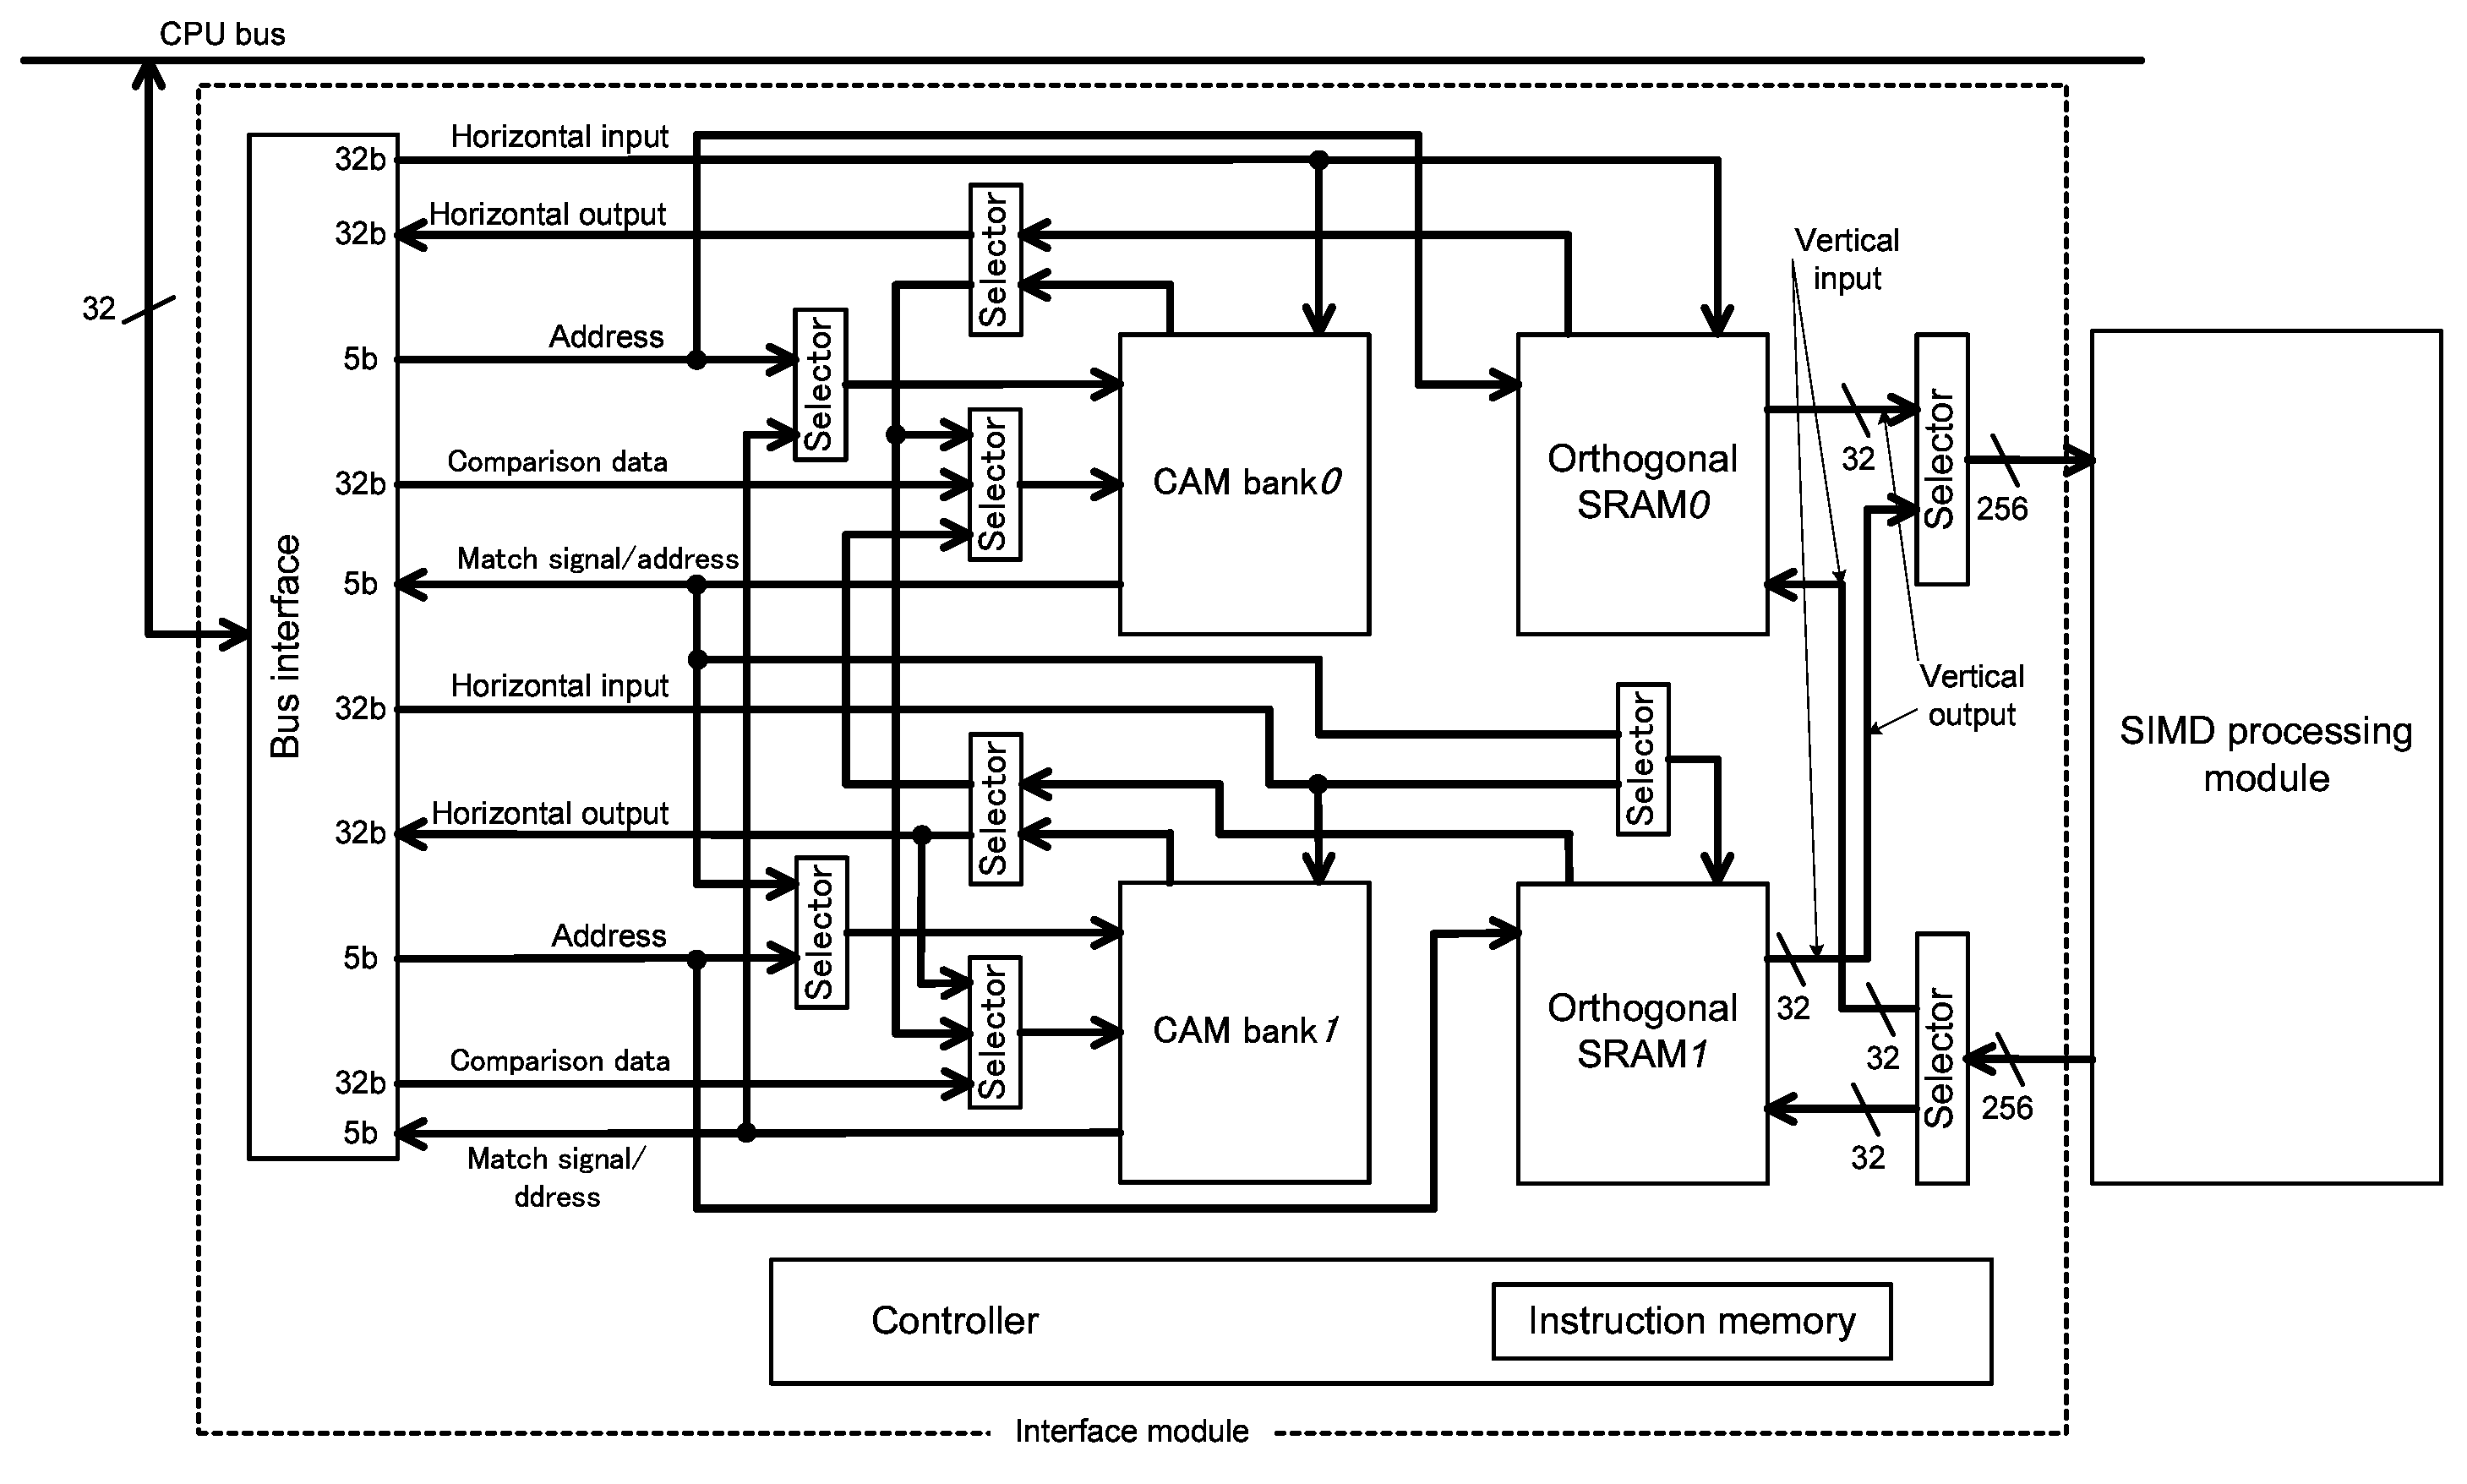
\includegraphics[width = 14cm,  height = 14cm, keepaspectratio, clip]{./pics/mtb_blk.eps}
		\end{center}
		\caption{テーブルルックアップインタフェースモジュールのブロック図.}
%		\ecaption{FMCAM with $d$ bits $\times$ $2^a$ words.}
		\label{mtb_blk}
	\end{figure}%	
%figure	

\subsubsection{直交SRAM}
\label{lbl_cp5_mtb_arch_hvsram}
基本動作及び構成は,\ref{lbl_cp5_mta_simd_mod}節で述べたものと同様に,
直交SRAMを2つ用意し,インターリーブ動作を実行する.
周辺にはCAMに対して,
水平に読み出したデータを転送し,検索結果を入力する配線が追加されている.

直交SRAMを2つ配置することで,第1案と同様のインターリーブ直交変換を行うことが可能であり,
さらにテーブル検索処理を行うCAMを独立して配置することにより,直交変換と
テーブル変換を同時に行うことを可能とした.

\subsubsection{CAM}
\label{lbl_cp5_mtb_arch_cam}

CAMを用意して,テーブルルックアップ符号化を高速に行う.
CAMのサイズはハフマン符号化を主体としたテーブルルックアップ符号化を
考慮して32 bit $\times$ 512 wordとなっており,
高速に一致検索処理を行うことができる.
CAMの内部は2バンク構成となっており,テーブルルックアップ処理の際には
1バンクごと独立の処理を行うことも可能である.
すなわち,同時に別々の検索データを受け取り一致検索処理
が可能であり,一方をCAMとして,もう一方をRAMとして動作させることができる.
従ってテーブルルックアップ処理の際にはバンク0に符号化前の全パターンを格納し,CAM
として動作させ,バンク1にはハフマンコードテーブル等のデータを格納し,RAMとして
動作させる.
また,この時処理される符号後のデータは,直接バスインターフェースを介してCPUへ送信する,
もしくは再び直交メモリへ返すことが可能である.

\subsubsection{コントローラ}
\label{lbl_cp5_mtb_arch_cnt}

直交SRAMとCAMの組み合わせは,高速な一致検索能力を利用して,テーブルルックアップ処理をはじめとする
様々な処理を行えることが期待できる.
そのため,アーキテクチャをプログラブルな構成とし,各種のアプリケーションを処理できる
仕様としたほうが望ましい.
%また,CPUとのインターフェース内部に位置しているため超並列SIMDプロセッサにデータを
%転送する際の,超並列SIMDプロセッサの制御も行う.
従って,コントローラ内部には命令メモリを備え,直交SRAM及びCAMを自在に制御できる仕様とした.
図 \ref{mtb_cnt}に,コントローラのブロック図を示す.

コントローラは以下に示す9種類の回路から構成される.

%figure
	\begin{figure}[tbh]
		\begin{center}
			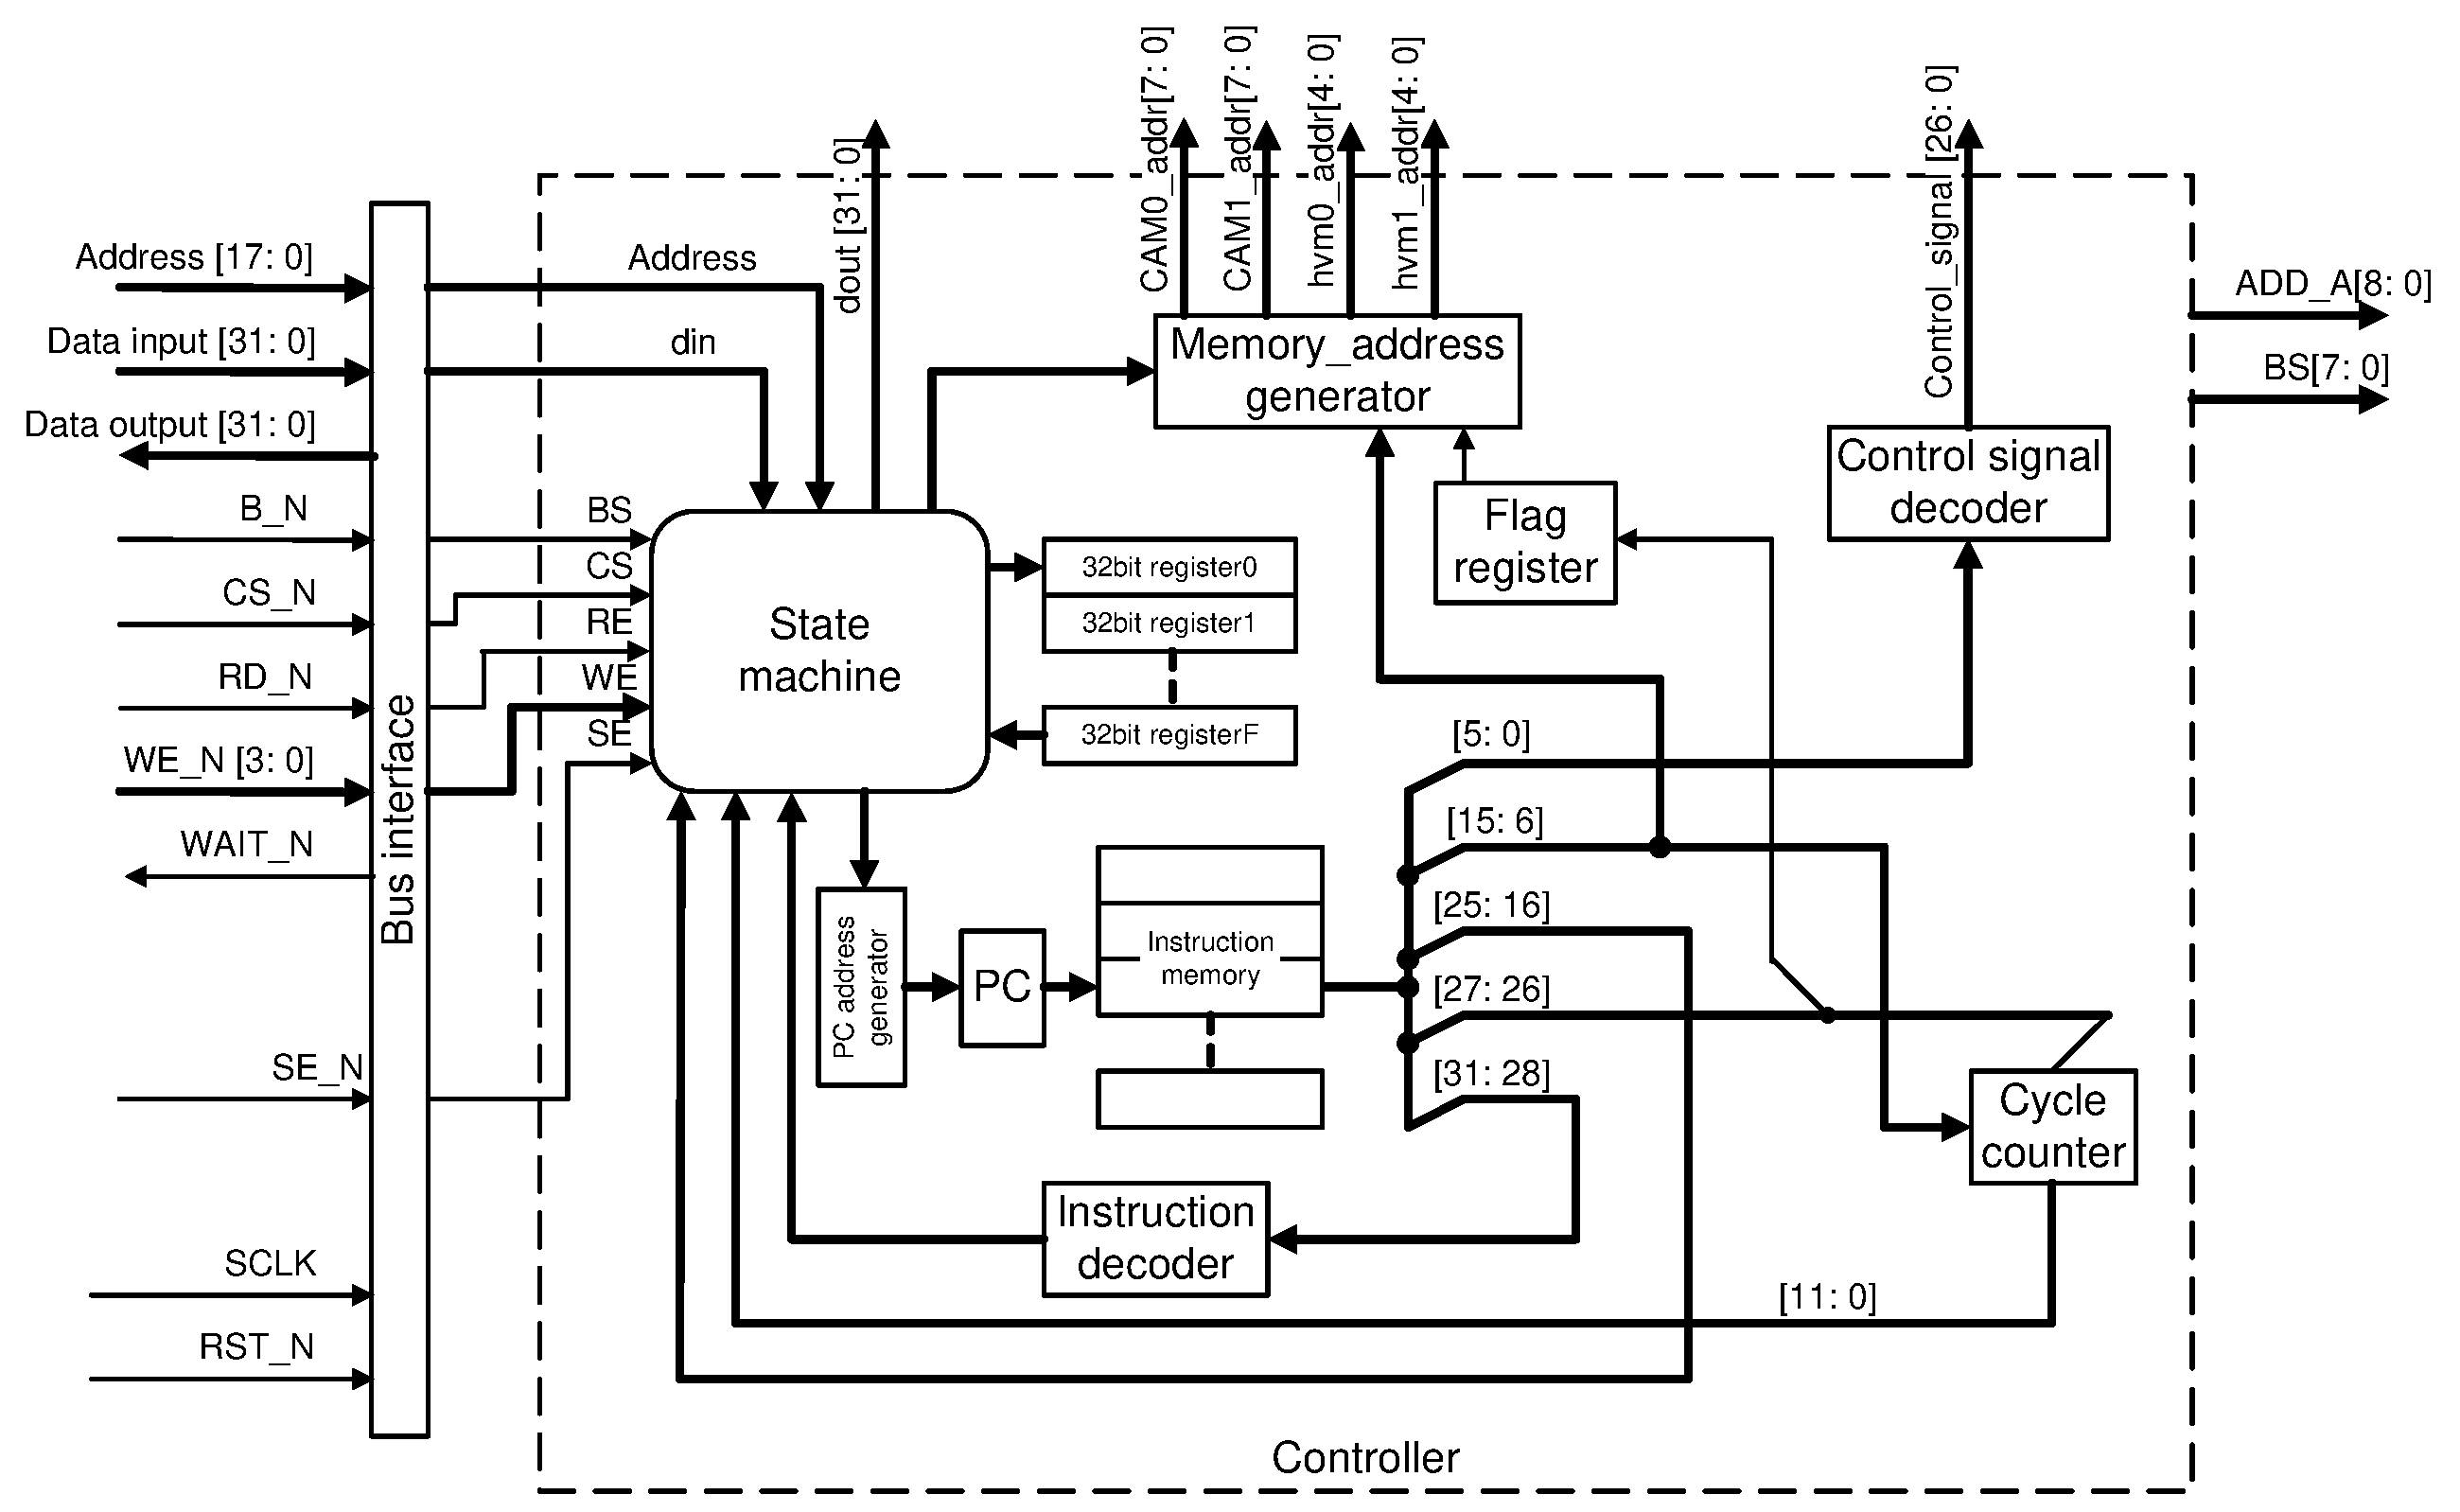
\includegraphics[width = 14cm,  height = 14cm, keepaspectratio, clip]{./pics/mtb_cnt.eps}
		\end{center}
		\caption{テーブルルックアップインターフェースコントローラブロック図.}
%		\ecaption{FMCAM with $d$ bits $\times$ $2^a$ words.}
		\label{mtb_cnt}
	\end{figure}%	
%figure	

\begin{itemize}
\item ステートマシン (State machine)  $\times$  1

		命令メモリから読み出されるデータを解釈し,コントローラ内部のその他の回路を制御する.

\item 命令メモリ (Instruction memory)  $\times$  1

		32 bit $\times$ 256 wordのメモリである.各ワードは,命令セット,デスティネーションアドレス,各種フラグ,及びその他の制御信号から
		構成されている.

\item 32ビットレジスタ (32 bit register)  $\times$  16 

		ステートマシンが使用するレジスタが用意されている.命令メモリに基づいて各回路,及びモジュールの
		制御信号やテンポラリデータが書き込まれる.

\item プログラムカウンタ及びプログラムカウンタアドレスジェネレータ (Program counter \& Program counter address generator)  $\times$  1

		プログラムカウンタから逐次アドレスが出力され,命令メモリ内のデータを読み出す.
		命令メモリから出力されたデータはステートマシンで解釈され,\ref{lbl_cp5_cmd_set}節にて示す
		ジャンプ命令等の場合には,
		プログラムカウンタアドレスジェネレータがカウンタ値を制御することとなる.

\item メモリアドレスジェネレータ (Memory address generator)  $\times$  1

		ステートマシンから出力されたデータに基づき,直交SRAM,及びCAMに入力されるアドレスをデコードして出力する.

\item フラグレジスタ (Flag register)  $\times$  1

		メモリアドレスジェネレータ制御用フラグ.

\item 命令セットデコーダ (Instruction decoder)  $\times$  1
	
		命令メモリから出力されたデータがこのデコーダを介することにより,命令セットに解釈され,
		ステートマシンの制御信号となる.

\item コントロールシグナルデコーダ (Control signal decoder)  $\times$  1

		直交SRAM,及びCAMの周辺回路を制御するための信号を出力する.

\item サイクルカウンタ (Cycle counter)  $\times$  1

		ループ回数等を記憶するカウンタ.

\end{itemize}


主な入出力ピンの役割は以下の通りである.

\begin{itemize}
\item SCLK (入力)

		CAMベース超並列プロセッサのマスタークロック

\item RST\_N (入力)
		
		CAMベース超並列プロセッサのグローバルリセット (非同期)

\item Address (入力)

		CAMベース超並列SIMD型プロセッサのアドレスである.
		テーブルルックアップインターフェースのコントローラは,内部のCAM,及び直交SRAMを
		制御すると同時に,SIMD型演算モジュール内のコントローラを制御しなければならない.
		図 \ref{mtb_spc}に,CAMベース超並列SIMD型プロセッサ全体のアドレス空間を示す.
		外部とのアクセスはこのアドレス空間を介して行う.
		色づけしてある箇所は,テーブルルックアップインターフェースのアドレス空間で,色付けされていない箇所は
		超並列SIMD型演算モジュールのアドレス空間である.

%figure
	\begin{figure}[tbh]
		\begin{center}
			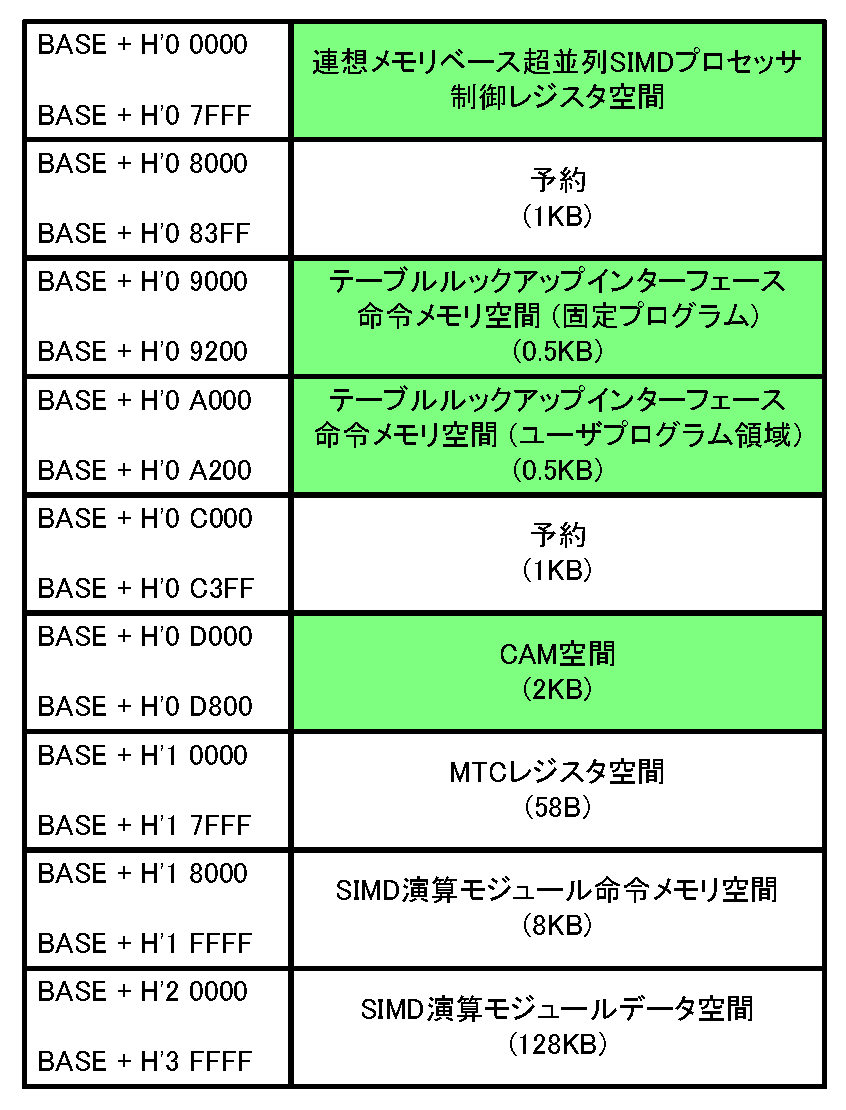
\includegraphics[width = 12cm,  height = 12cm, keepaspectratio, clip]{./pics/mtb_spc.eps}
		\end{center}
		\caption{超並列SIMD型プロセッサのメモリ空間.}
%		\ecaption{FMCAM with $d$ bits $\times$ $2^a$ words.}
		\label{mtb_spc}
	\end{figure}%	
%figure	

\item Data input (入力)

		CPUからCAMベース超並列SIMD型プロセッサへの32 bitデータ入力

\item Data output (出力)

		CAMベース超並列SIMD型プロセッサからCPUへの32 bitデータ出力

\item CS\_N (入力)

		CPUが,CAMベース超並列SIMD型プロセッサを選択するための信号

\end{itemize}

コントローラのアーキテクチャは,命令メモリにプログラムを格納し,
取り扱うデータは直交SRAM及びCAMに格納される構成とした.
これは,ハーバードアーキテクチャの1種であり,フォン・ノイマンボトルネックの解消を実現している.


\subsubsection{バスインターフェース}
\label{lbl_cp5_mtb_arch_bus}
基本動作及びその処理は,\ref{lbl_cp5_mta_simd_mod}
にて述べたものと同様である.

\subsection{命令セット}
\label{lbl_cp5_cmd_set}

テーブルルックアップインタフェースモジュールは,内部の命令メモリに
プログラムを格納することで,直交SRAM,及びCAMを用いた様々な処理を
行うことができるように設計した.
命令長は,今後の拡張を考慮して冗長度の高い32 bitとしている.
図 \ref{inst_fld}に示すのが,1命令のフィールド構成となる.
LSBから,5 bitは直交SRAM,及びCAMのイネーブル信号を制御するフィールドであり,
コントロールシグナルデコーダにて制御信号に変換される.
6 bitから15 bitまでは,直交SRAM,及びCAMに入力するアドレスとなる.
16 bitから25 bitまでは,後述する命令セットで使用される,デスティネーションアドレスやループ回数を格納する.
26 bitから27 bitまでは,フラグを格納するフィールドである.
27 bitから31 bitまでは,命令コードを格納し,命令セットデコーダによって変換されコントローラの動作を決定する.

 以下にプログラムを作成するための,基本命令セットを示す.

%figure
	\begin{figure}[tbh]
		\begin{center}
			\includegraphics[width = 14cm,  height = 14cm, keepaspectratio, clip]{./pics/inst_fld.eps}
		\end{center}
		\caption{テーブルルックアップインタフェースモジュールの命令フィールド構成.}
%		\ecaption{FMCAM with $d$ bits $\times$ $2^a$ words.}
		\label{inst_fld}
	\end{figure}%	
%figure	

\begin{enumerate}
\item \texttt{NO OPERATION}:

	テーブルルックアップインターフェース制御コードを出力し,PC (Program Counter)を1つ進ませる.

\item \texttt{INITIALIZE}

	コントローラ内のレジスタを初期化しPCのアドレスを0にする.

\item \texttt{LOOP}

	この命令が格納されているアドレスの次のアドレスから,Return命令 (後述)が格納されている
アドレスまで指定された回数分処理を繰り返す.

\item \texttt{RETURN}

	ループ命令における繰り返し処理の最後に実行する.この命令が実行されるとループ命令が
位置しているアドレスの次のアドレスにPCが移動する.また,この際にループ回数が1つ減る.

\item \texttt{JUMP} (\texttt{NO CONDITION})

	デスティネーションアドレスフィールドで示されたアドレス (プログラム開始アドレスを
ベースアドレスとする)に無条件でジャンプする.

\item \texttt{JUMP} (\texttt{CONDITION})

	条件が真である場合,デスティネーションアドレスフィールドで示されたアドレスにジャンプする.
	偽である場合はアドレスをインクリメントする.

\item \texttt{STAY}

	この命令が格納されている動作を実行し,PCの値は保持する.主にCPUからの制御信号で使用 (\ref{lbl_cp5_mta_proc_io}節で示す,スルーモード等).

\item \texttt{HALT}

	この命令が実行された場合,プログラムの処理が終了となる.
\end{enumerate}

\subsection{動作概要}
\label{lbl_cp5_mta_proc}

\ref{lbl_cp5_mtb_arch}節にて,CAMベーステーブルルックアップ符号化アーキテクチャをインタフェースモジュールに
組み込むアーキテクチャを示した.
この章では,テーブルルックアップインターフェース動作の基本となる,
データ入出力の手順やテーブルルックアップ符号化処理の手順を示す.

\subsubsection{データ入出力}
\label{lbl_cp5_mta_proc_io}

CPUからテーブルルックアップインターフェースを介して,CAMベース超並列SIMD型プロセッサに
データを書き込む,もしくは読み出す場合は,データを直交変換する動作 (以下,直交モードと呼ぶ)と,
直接書き込む動作 (以下,スルーモードと呼ぶ)の
2通りが考えられる.
従ってコントローラはそれぞれの場合に応じて直交SRAM,CAM及びSIMD型演算処理部を
制御しなければならない.以下に処理の流れを示す.

\begin{itemize}

\item 直交モード

これは,通常使用されるモードで,CPUとSIMD型演算モジュールとのデータの入出力及び,
テーブルルックアップインタフェースモジュールを使用してのアプリケーション処理に利用される.
処理の流れを,図 \ref{wrt_flw}に示す.
処理の開始時にはCPUから,CAMベース超並列SIMD型プロセッサ制御レジスタ空間にあるコンフギュレーション
レジスタを``0"に設定する.
次に,書き込みもしくは読み出し用のアドレス設定レジスタに,処理開始アドレスを書き込む.
その後,ライトバッファレジスタかリードバッファレジスタに``1"を書き込むことで,CPUからバースト書込み,
もしくは読み出しが可能となる.

\item スルーモード

このモードは,CAMとSIMD型演算モジュール間で,直交変換を施さず
データを送受信する,及び各種レジスタプログラムの書込みに使用されるモードである.
図 \ref{wrt_flw}に示すように,始めにコンフギュレーションレジスタを``1"に設定する.
その後,リードイネーブルもしくはライトイネーブルを制御しアドレスもしくはアドレスと書き込みデータを
入力することで,データの読み出し,書き込みが可能となる.
\end{itemize}



%figure
	\begin{figure}[tbh]
		\begin{center}
			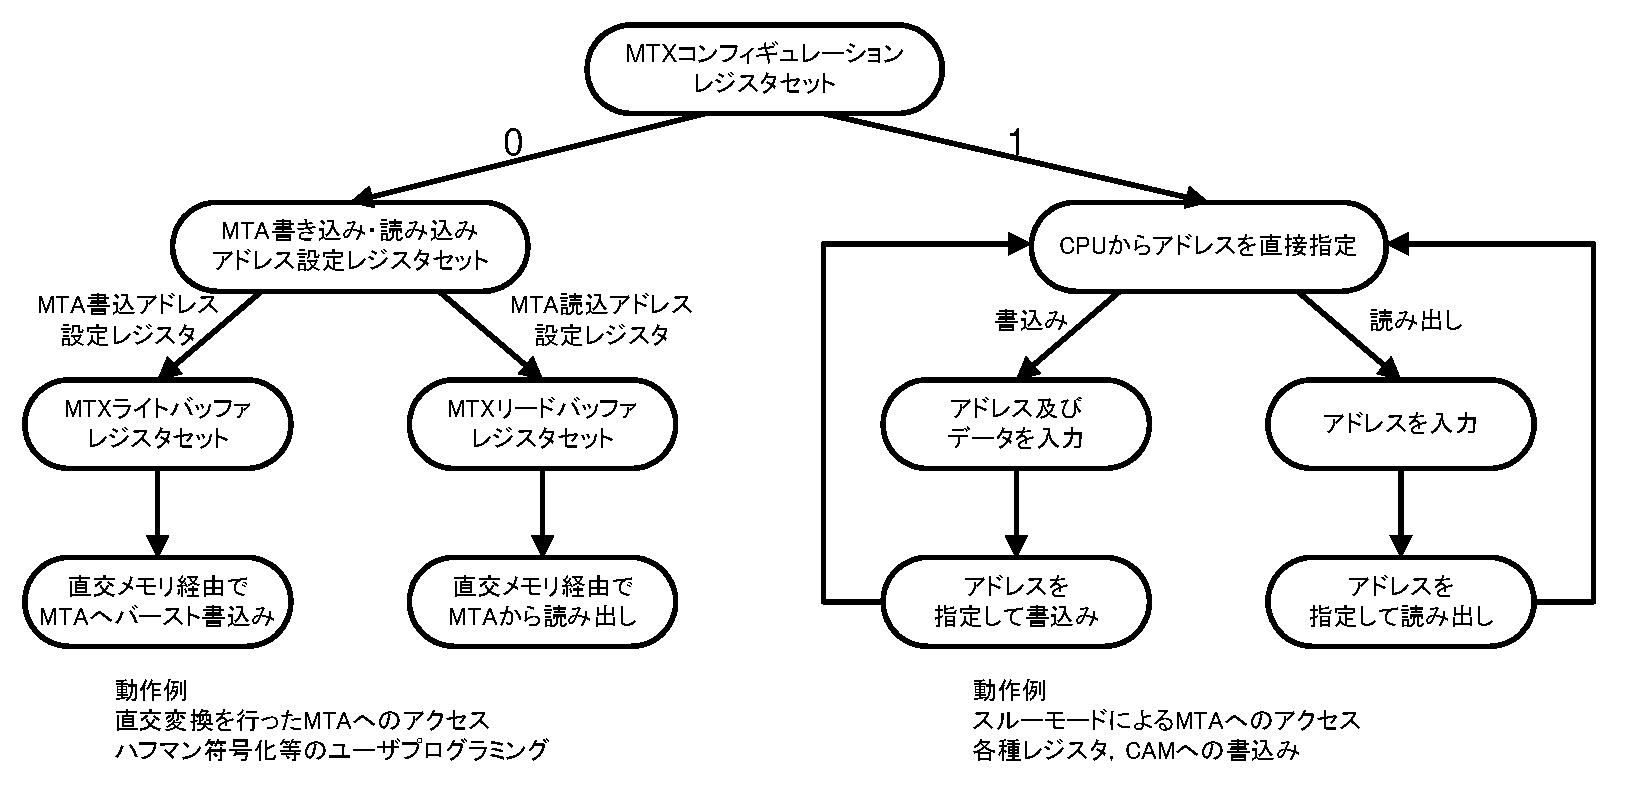
\includegraphics[width = 14cm,  height = 14cm, keepaspectratio, clip]{./pics/wrt_flw.eps}
		\end{center}
		\caption{テーブルルックアップインタフェースモジュールを利用したデータ処理フロー.}
%		\ecaption{FMCAM with $d$ bits $\times$ $2^a$ words.}
		\label{wrt_flw}
	\end{figure}%	
%figure	


\subsubsection{テーブルルックアップ符号化}

テーブルルックアップ処理は,符号後のデータを直接CPUへ送信する処理と
再び,SIMD型演算モジュール内にフィードバックする処理の2通りが考えられる.
以下にそれぞれについて詳述する.

\begin{itemize}

\item ハフマン符号化処理の例
\label{lbl_cp5_mta_proc_huff}

ハフマン符号化は,画像処理のプロセスにおける最後のアルゴリズムとして使用されることが多い.
従って,超並列SIMD型プロセッサで処理されたマルチメディアデータは,
符号化前データとして直交SRAMを介してCAMへ転送される.
その後テーブルルックアップ処理が行われて,CPUへ出力される.
具体的な処理は,図 \ref{mtb_huff}に示す,\ding{"C0}から\ding{"C5}の順で行われる.
直交SRAM$0$及び直交SRAM$1$をデータのインターリーブ直交変換に使用し,
CAMバンク$0$及びCAMバンク$1$をテーブル検索に利用することによって
完全パイプラインのハフマン符号化が実現される.
CAMバンク$0$には,入力される符号化前データの全パターンを格納し,
CAMバンク$1$には,ハフマン符号化テーブルを格納する.
なお,ここで示すハフマン符号化は基礎技術となる静的ハフマン符号化の例であり.
リアルタイム符号化テーブル最適化アルゴリズムを適用していない.

%figure
	\begin{figure}[tbh]
		\begin{center}
			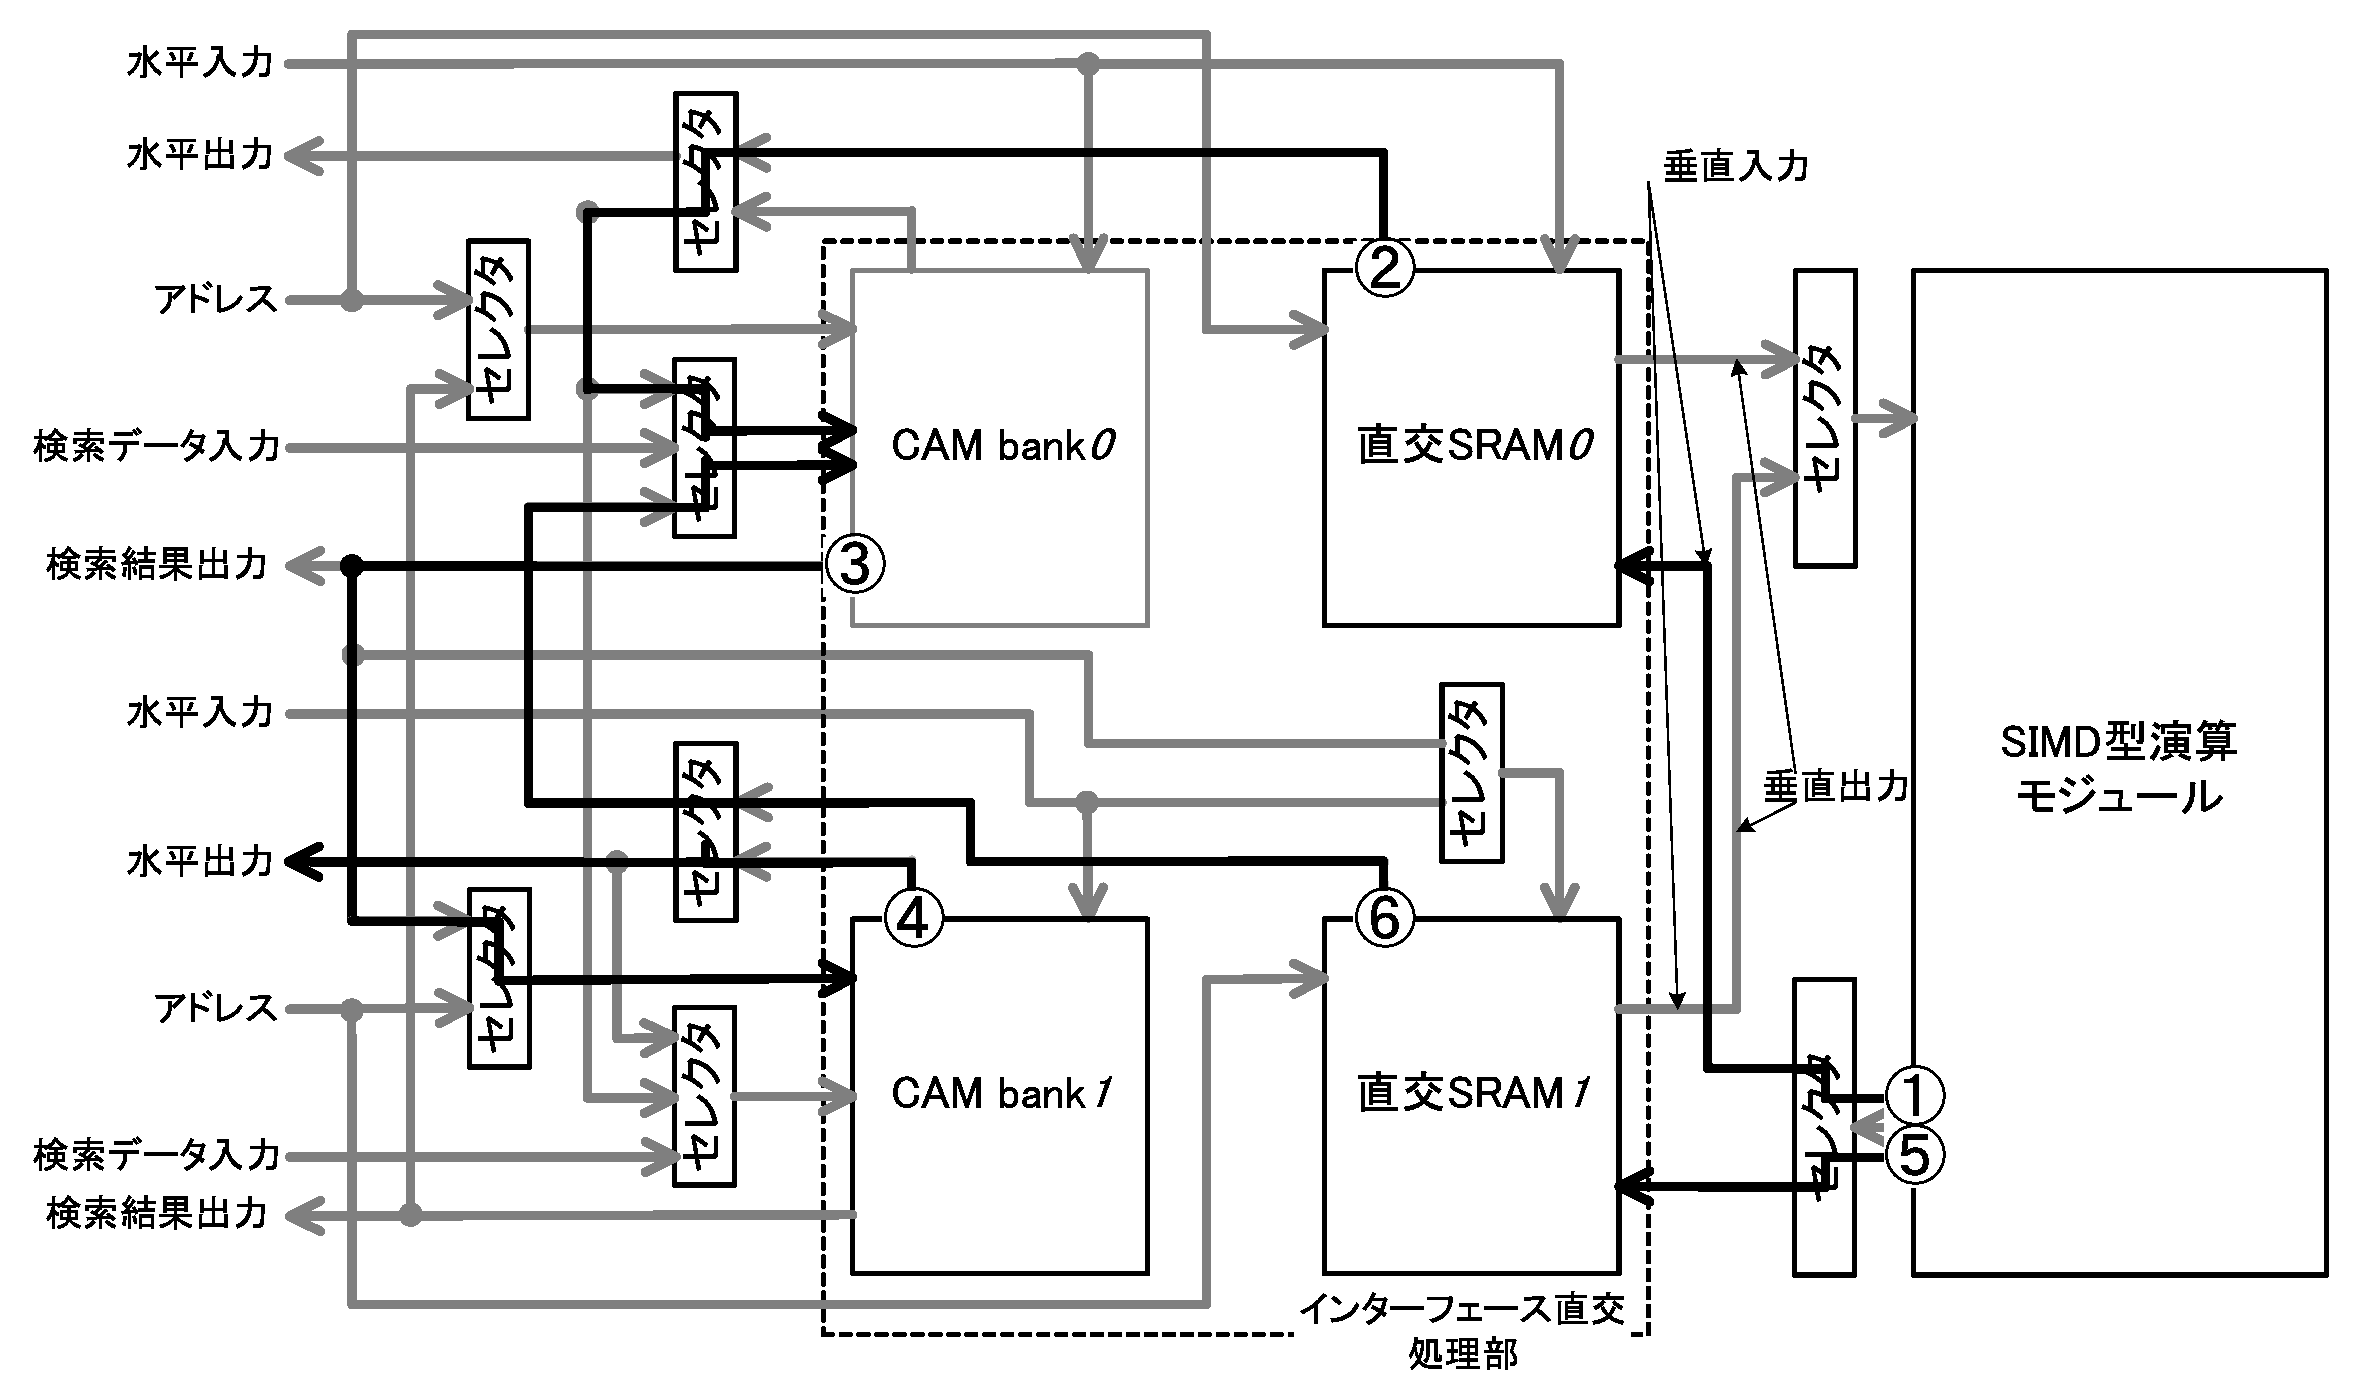
\includegraphics[width = 14cm,  height = 14cm, keepaspectratio, clip]{./pics/mtb_huff.eps}
		\end{center}
		\caption{インタフェースモジュールによるハフマン符号化の例.}
%		\ecaption{FMCAM with $d$ bits $\times$ $2^a$ words.}
		\label{mtb_huff}
	\end{figure}%	
%figure	

\begin{enumerate}
\item[{\ding{"C0}}] 超並列SIMD型プロセッサから,1 bit毎データを読み出し直交SRAM$0$に垂直入力する
\item[{\ding{"C1}}] \ding{"C0}で格納されたデータを,アドレスの降順に水平読み出しし,読み出されたデータをCAMバンク$0$に
						検索データとして入力する.
\item[{\ding{"C2}}] CAMバンク$0$には,あらかじめハフマンコードが格納されているため,入力される検索データと一致する
					ハフマンコードが検索され,そのアドレスが出力される.
\item[{\ding{"C3}}] \ding{"C2}で出力されたアドレスをCAMバンク$1$に,水平方向のアドレスとして入力する.
					CAMバンク$1$には,あらかじめ符号後のデータがCAMバンク$0$のハフマンコードとアドレスで対応付けされて格納されており,
					その出力から,符号後データを得る.
\item[{\ding{"C4}}] 直交SRAM$0$が符号前データをCAMバンク$0$に出力している間に,直交SRAM$1$には超並列SIMD型プロセッサから
					1 bit毎データが垂直入力される.
\item[{\ding{"C5}}] \ding{"C1}と同様の操作で直交SRAM$1$から,CAMバンク$0$に検索データを出力する.
					その後は\ding{"C2}と同様のプロセスを経て符号後のデータが出力される.
					なお,この間直交SRAM$0$には,\ding{"C0}の処理が行われることとなる. 
\end{enumerate}


\item 暗号処理の例
\label{lbl_cp5_mta_proc_aes}

前述の例では,CAMによる一致検索機能をテーブルルックアップ処理の一種であるハフマン符号化処理に応用し,
その処理結果をCPUへ直接出力する方法について述べた.
一般に,マルチメディアアプリケーションは,ハフマン符号化の様に,CAMの処理結果を直接CPUへ出力するものと,
%誤り訂正符号化のアルゴリズムであるLDPC (Low Density Parity Check code)や,暗号処理であるAES (Advanced EnC$_r$yption Standard)の様に,
アルゴリズムの途中にテーブルルックアップ符号化を行い,その結果を再度超並列SIMD型プロセッサへフィードバックするものがある.
この処理で代表的なものは,暗号化がありAESアルゴリズムは,繰り返し演算処理の間にSub byte変換というテーブルルックアップ処理が
行われる.具体的な処理は,図 \ref{mtb_aes}に示す,\ding{"C0}から\ding{"C3}の順で行われる.

\begin{enumerate}
\item[{\ding{"C0}}] 超並列SIMD型プロセッサから,1 bit毎データを読み出し,直交SRAM$0$に垂直入力する.
\item[{\ding{"C1}}] \ding{"C0}で格納されたデータを,アドレスの降順に水平読み出しし,読み出されたデータをCAMバンク$0$に検索データとして入力する.
\item[{\ding{"C2}}] CAMバンク$0$に格納されているデータと検索処理が行われ,入力される検索データと一致した場合,そのアドレスが出力されることとなる.
					出力されたアドレスは,直交SRAM$1$に,水平入力のデータとして入力される.
\item[{\ding{"C3}}] 直交SRAM$1$の全アドレスに,\ding{"C2}の処理で入力されたデータが格納されたならば,超並列SIMD型プロセッサへ,
						1 bit毎データを出力する.
\end{enumerate}

 なお,上記の処理において,CAMバンク0は一致検索処理を行ったが,単なるメモリとして機能させても良い.

%figure
	\begin{figure}[tbh]
		\begin{center}
			\includegraphics[width = 14cm,  height = 14cm, keepaspectratio, clip]{./pics/mtb_aes.eps}
		\end{center}
		\caption{インタフェースモジュールによるフィードバック処理の例.}
%		\ecaption{FMCAM with $d$ bits $\times$ $2^a$ words.}
		\label{mtb_aes}
	\end{figure}%	
%figure	

\end{itemize}

\subsection{VLSI実装結果}
\label{lbl_cp5_impl}

CAMベーステーブルルックアップ符号化アーキテクチャを融合させた,超並列SIMD型プロセッサ
のインタフェースモジュールを,90 nm CMOS技術によって開発した.
アーキテクチャはハードウェア技術言語 (HDL: Hardware Description Language)の一種である,Verilog-HDL
を用いて開発した.表 \ref{mtb_impl_sft}に,ソフトマクロでの論理合成結果を示す.
使用ツールは,シノプシス社のDesign Compiler (バージョン2005.09)を使用した.
動作周波数の制約は,超並列SIMD型プロセッサの動作周波数に合わせるために200 MHzとした.
また,最小面積を目標として合成されるように制約を施している.
論理合成後の,全体面積は約0.75 mm$^2$となった.
%これは主に,直交SRAM2つ,CAMを2つ,及びコントローラによって構成されている.
直交SRAMは	32 bit $\times$ 32 wordとサイズが小さいため,約0.03 mm$^2$と,最も小さかった.
次いでコントローラが約0.21 mm$^2$というサイズであり,最も大きい32 bit $\times$ 256 wordのCAMサイズ約0.24 mm$^2$
と近い値になったが,これは,命令メモリサイズ (32 bit $\times$ 256 word)を,大きめに備えているためである.

ここで直交SRAMとCAMをフルカスタムで設計した場合の実装に関して面積の見積もりを算出する.
ベースとなるVerilogソースに,フルカスタムによるメモリ類を実装した場合の論理合成見積もりを表 \ref{mtb_impl_hrd}に示す.
直交SRAMは図 \ref{hv_cell}に示す直交SRAMセルのレイアウト,及び図 \ref{hv_ary}に示す直交SRAMセルアレイを元に面積を算出した.
一般的にメモリモジュールのセル以外の周辺回路はセルエリアの約50\%程度と見積もることができるため.
算出した結果,約0.01 mm$^2$と見積もることができた.
また,CAMに関しては直交SRAMセルのサイズとCAMセルのサイズが
ほぼ1対1であることが分かっているので,面積を約0.08 mm$^2$と見積もった.
その結果,全体の面積は約0.39 mm$^2$となり,ソフトマクロ実装の場合の約2分の1となった.
なお,命令メモリをフルカスタム化することで,更なる面積の削減を実現することが可能である.
超並列SIMD型プロセッサの面積が,3.1 mm$^2$であるので
CAMベース超並列SIMD型プロセッサは,約3.49 mm$^2$
となった.一般にモバイル機器向けのSoCのコアが約1 cm$^2$であることを考慮すると,
十分実装できる大きさであることがわかる.


%figure*
	\begin{table}[thb]
	\centering
		\begin{center}
		\caption{ソフトマクロによる,テーブルルックアップインタフェースモジュールの実装結果.}
%			\includegraphics[width = 8.5cm, height = 8.5cm, keepaspectratio, clip]{impl_rslt.eps}
			\includegraphics[width = 12cm, height = 12cm, keepaspectratio, clip]{./pics/mtb_impl_sft.eps}
		\label{mtb_impl_sft}
		\end{center}
	\end{table}%
%figure*

%figure*
	\begin{table}[thb]
	\centering
		\begin{center}
		\caption{ハードマクロによる,テーブルルックアップインタフェースモジュールの実装結果.}
%			\includegraphics[width = 8.5cm, height = 8.5cm, keepaspectratio, clip]{impl_rslt.eps}
			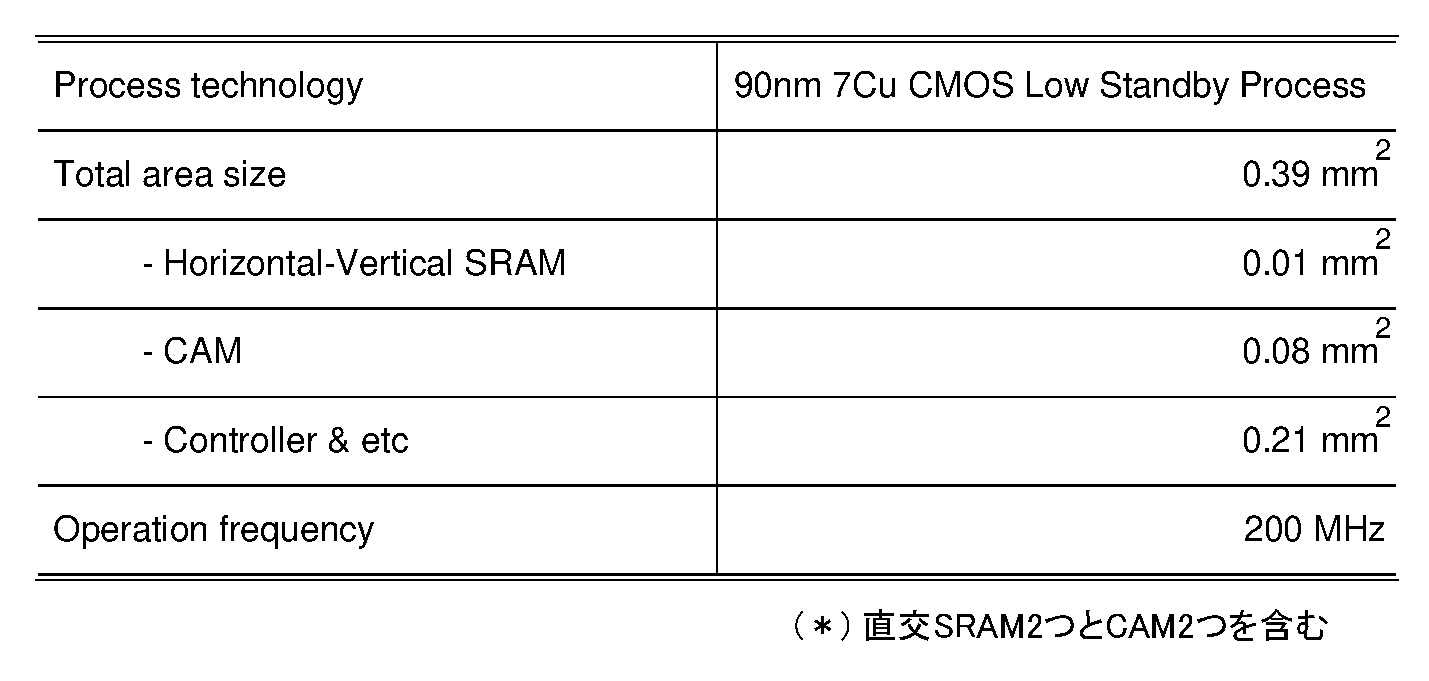
\includegraphics[width = 12cm, height = 12cm, keepaspectratio, clip]{./pics/mtb_impl_hrd.eps}
		\label{mtb_impl_hrd}
		\end{center}
	\end{table}%
%figure*

%figure
	\begin{figure}[tbh]
		\begin{center}
			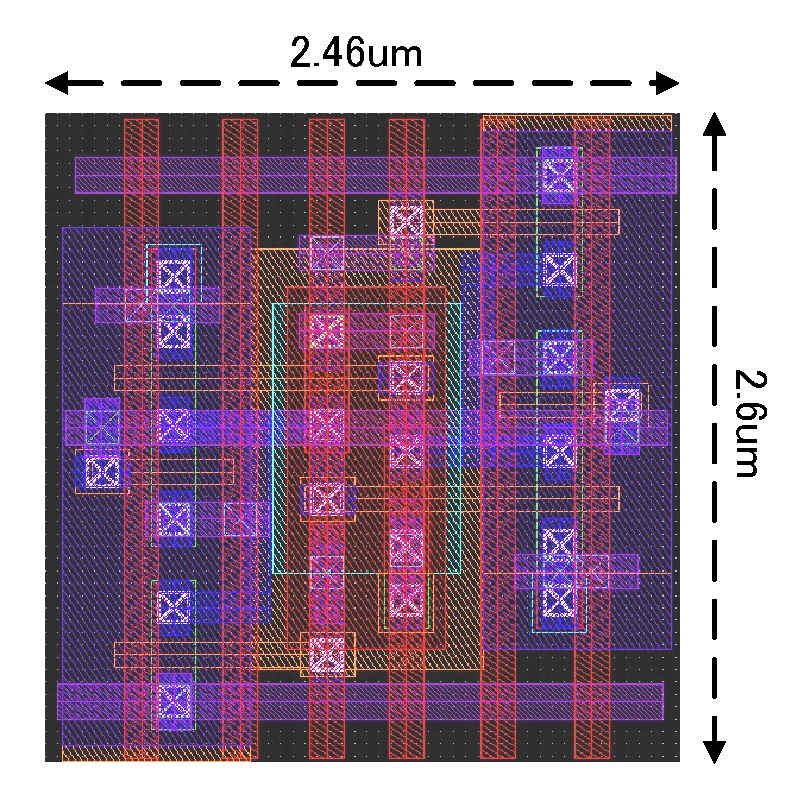
\includegraphics[width = 12cm,  height = 12cm, keepaspectratio, clip]{./pics/hv_cell.eps}
		\end{center}
		\caption{直交SRAMセルのレイアウト.}
%		\ecaption{FMCAM with $d$ bits $\times$ $2^a$ words.}
		\label{hv_cell}
	\end{figure}%	
%figure	

%figure
	\begin{figure}[tbh]
		\begin{center}
			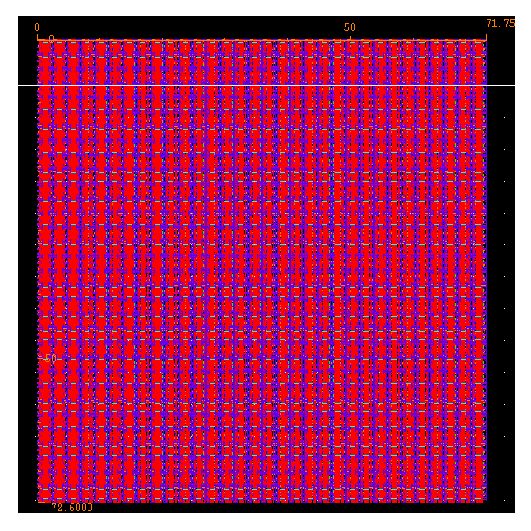
\includegraphics[width = 14cm,  height = 14cm, keepaspectratio, clip]{./pics/hv_ary.eps}
		\end{center}
		\caption{32 bit $\times$ 32 wordの直交SRAMセルアレイ.}
%		\ecaption{FMCAM with $d$ bits $\times$ $2^a$ words.}
		\label{hv_ary}
	\end{figure}%	
%figure	

\clearpage

\section{画像処理アルゴリズムへの適用}
\label{lbl_cp5_jpg}

この節では,CAMベース超並列SIMD型プロセッサを用いて,
マルチメディアデータ処理を行い,性能を評価する.
性能評価に用いるマルチメディアアプリケーションは,静止画像圧縮技術の1つであり,
カラー画像の国際標準方式に制定されている,JPEG (Joint Photographic Experts Group)アルゴリズムを用いる.

\subsection{JPEG方式の概要}
\label{lbl_cp5_jpg_siyo}
JPEG方式 (以下,JPEGと呼ぶ)は,デジタルカメラ等のデジタル家電や携帯電話等のモバイル機器で幅広く用いられており,
繰り返し演算やテーブルルックアップ符号化を含むマルチメディアアプリケーションである.
JPEGは,図 \ref{jpg_srs}に示すように基本方式 (Baseline system),拡張方式 (Extended system),
及びDPCM (Differential Pulse Code Modulation)と呼ばれる差分パルス符号化方式に分けることができる.
一般のモバイル機器や,デジタル家電で多く用いられているのは基本方式であり,DCT (Discrete Cosine Transform:離散コサイン変換)
をベースにしたDCT方式を利用して,高い圧縮率を実現する.
ただし,情報の一部が省略され,復号時には非可逆となるため,完全な画像の再現はできない.
これに対して,オプション機能として用意されているのが,拡張方式とDPCM方式である.
拡張方式は,算術符号化\cite{ohkjmz03}等を用いて,高精彩画像,及び高能率符号化を実現するものである.
DPCM方式は,画像の可逆方式を実現する,すなわちデータの欠損がない復号処理を行うアルゴリズムである.
これは,DCTを用いず,空間関数アルゴリズムを用いることによって実現され,主に医療診断用等の特殊な用途で使用される.
今回の評価では,CAMベース超並列SIMD型プロセッサのマルチメディアデータへの適用を
踏まえ,最も一般的な基本方式に基づいて性能評価を行う.
図 \ref{baseline}に,JPEGの基本処理フローを示す.
以下の節では,マルチメディアデータ処理LSIにとって処理の負担が大きい,DCTとハフマン符号化を中心として各処理の説明及び
CAMベース超並列SIMD型プロセッサアーキテクチャによる処理の概要について述べる.

%figure
	\begin{figure}[tbh]
		\begin{center}
			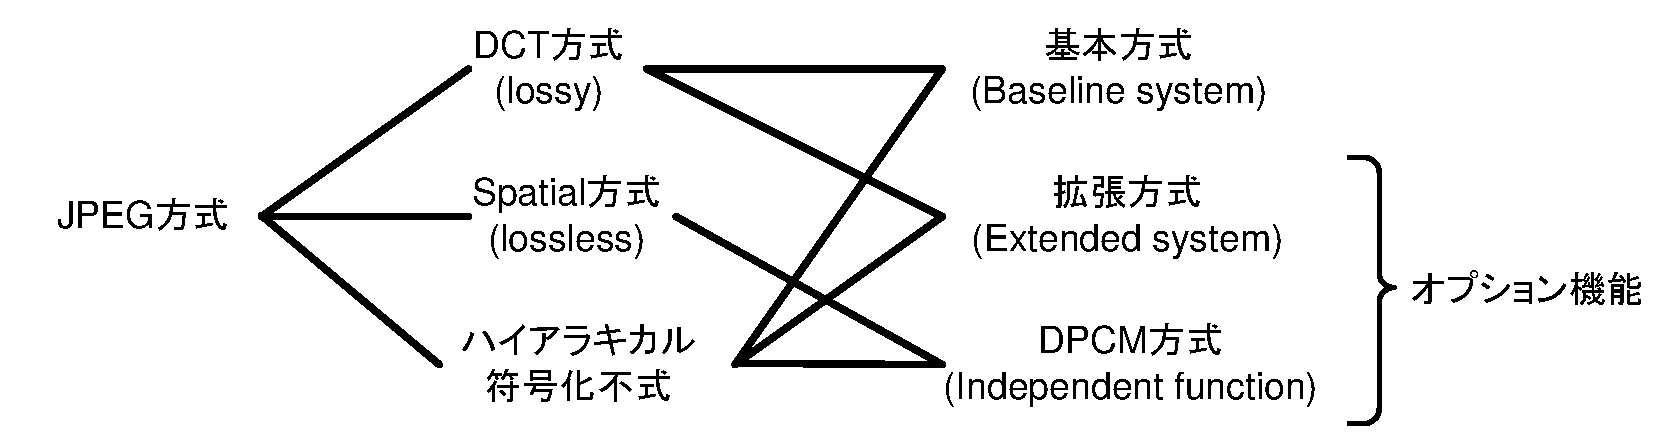
\includegraphics[width = 14cm,  height = 14cm, keepaspectratio, clip]{./pics/jpg_srs.eps}
		\end{center}
		\caption{JPEG方式の分類図.}
%		\ecaption{FMCAM with $d$ bits $\times$ $2^a$ words.}
		\label{jpg_srs}
	\end{figure}%	
%figure	

%figure
	\begin{figure}[tbh]
		\begin{center}
			\includegraphics[width = 12cm,  height = 12cm, keepaspectratio, clip]{./pics/baseline.eps}
		\end{center}
		\caption{JPEG基本方式の処理フロー.}
%		\ecaption{FMCAM with $d$ bits $\times$ $2^a$ words.}
		\label{baseline}
	\end{figure}%	
%figure	



\subsection{DCT (Discrete Cosine Transform)}
\label{lbl_cp5_jpg_dct}

DCT (Discrete Cosine Transform)は,離散コサイン変換とも呼ばれ,
画像内の各画素をコサイン波で表される周波数成分に変換して,
各画素値を各周波数成分にかかる係数 (DCT係数値)
で表す座標変換処理である
%\cite{xx}
.

ここで,今後の性能評価に関係のある,画像と周波数の関係について図 \ref{pic_fre}を例として述べることにする.
この例では簡単のために,画像は白か黒どちらかのみ使用している.
図中の上部にある画像を周波数 (空間周波数と呼ぶ)に変換すると,
下部のようになる.縦軸は色の濃淡を表し,黒に近いほど値は小さくなり,
白に近いほど値は大きくなる.また横軸は距離を表す.
従って,左の周波数は色の変化が少ないため
低い周波数となり,右の周波数は色の変化が激しく,高い周波数となる.
音が正弦波の重ねあわせで表現できるように,画像も基本周波数の重ねあわせで
表現できることになる.

%figure
	\begin{figure}[tbh]
		\begin{center}
			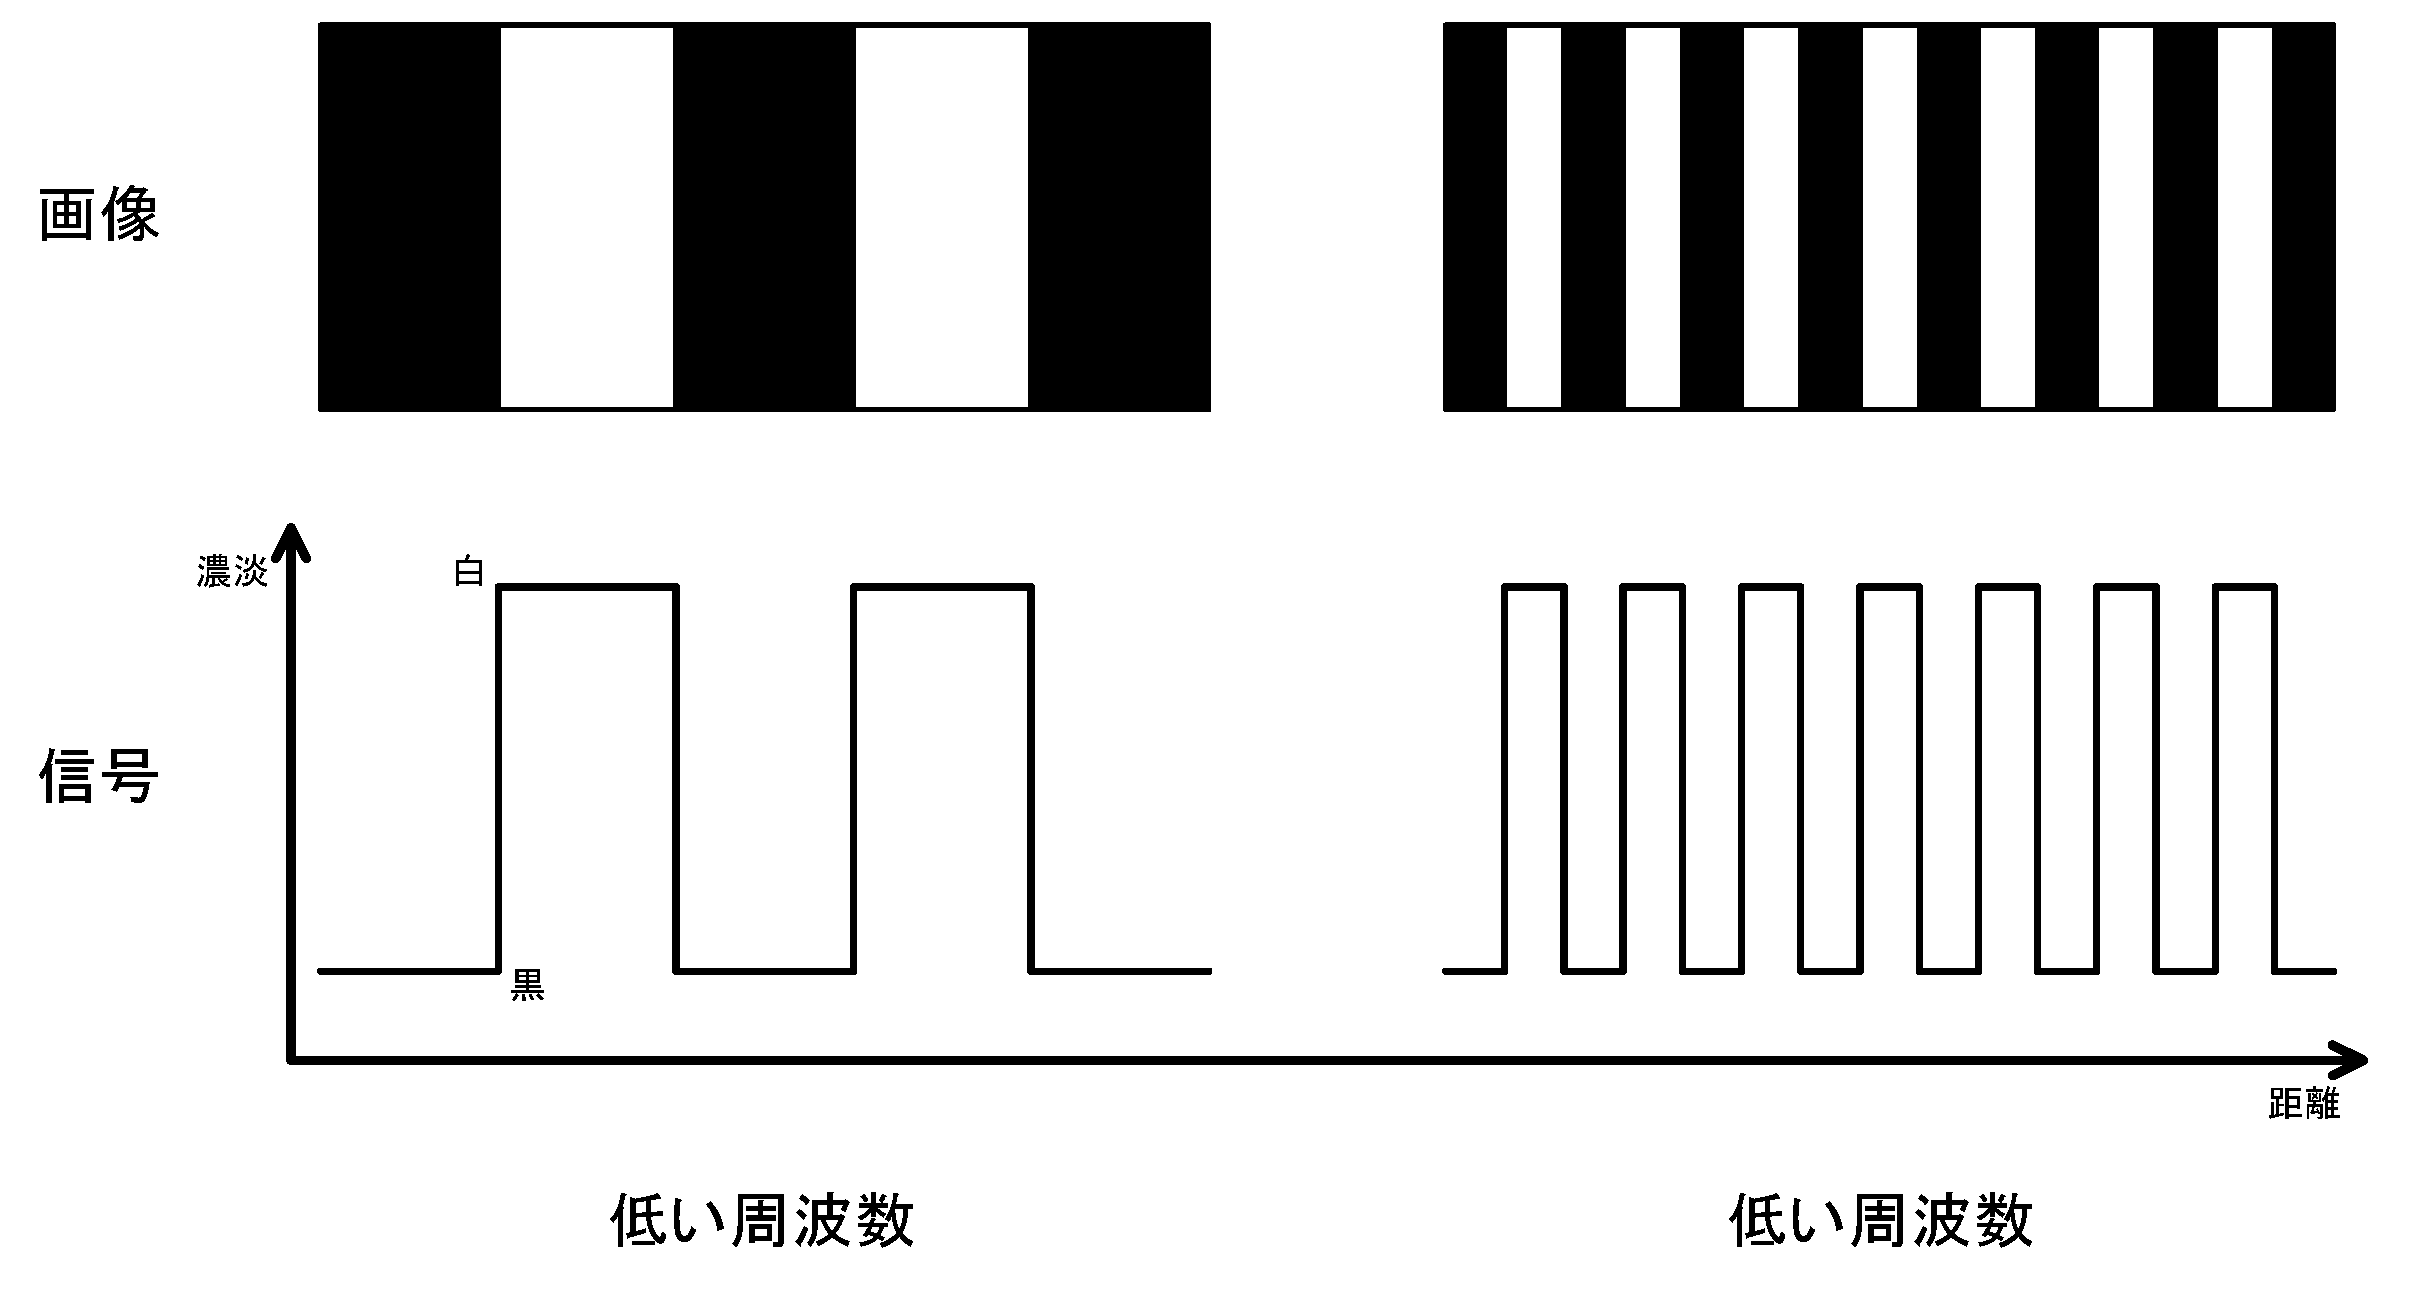
\includegraphics[width = 12cm,  height = 12cm, keepaspectratio, clip]{./pics/pic_fre.eps}
		\end{center}
		\caption{画像と周波数.}
%		\ecaption{FMCAM with $d$ bits $\times$ $2^a$ words.}
		\label{pic_fre}
	\end{figure}%	
%figure	

DCT処理は,N$_x$ $\times$ N$_y$ (N$_x$,N$_y$は,x,y方向の画素数)の画素値の集合を対象として
演算が行われる.この集合に施した結果は,
低周波数成分が左上に,高周波数成分が右下まとめられ,各画素値はDCT係数値で表される.
図 \ref{dct_pat}に,x及びyが8の場合のDCTの基本パターン群を示す.
これらのパターンが画像の中にどの程度含まれているかがDCTの結果表される.
その後,各画素の冗長な成分が量子化によって圧縮される.

%figure
	\begin{figure}[tbh]
		\begin{center}
			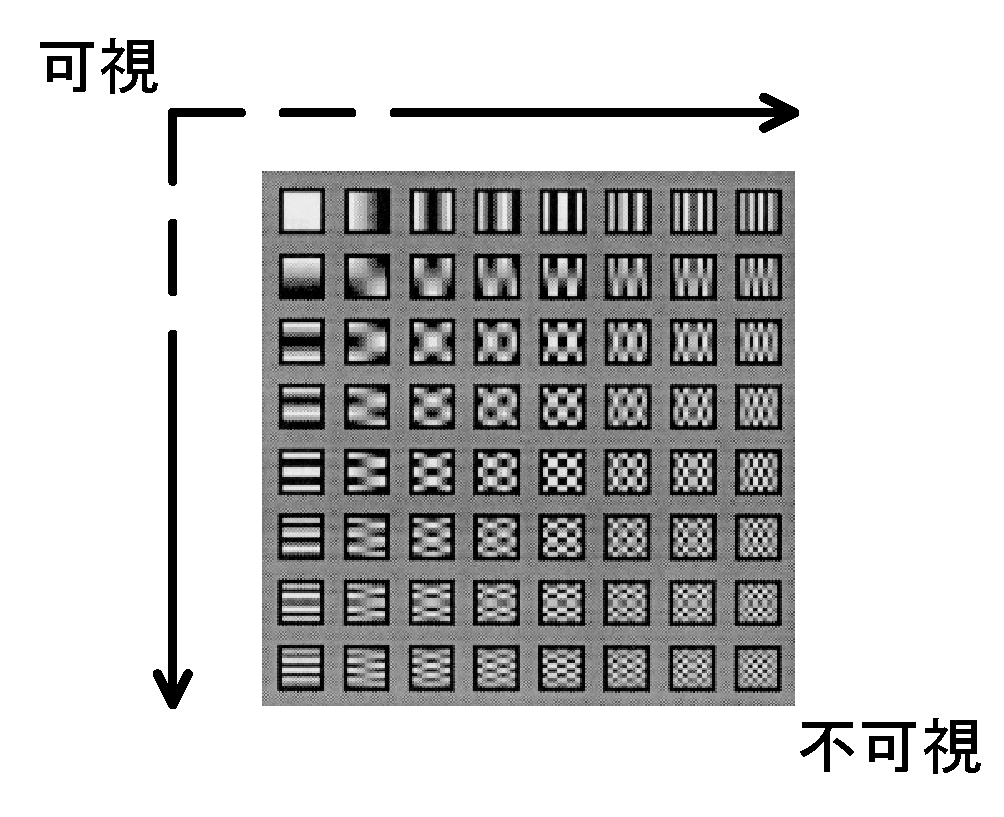
\includegraphics[width = 12cm,  height = 12cm, keepaspectratio, clip]{./pics/dct_pat.eps}
		\end{center}
		\caption{DCT基本パターン群.}
%		\ecaption{FMCAM with $d$ bits $\times$ $2^a$ words.}
		\label{dct_pat}
	\end{figure}%	
%figure	

DCT処理は,N$_x$ $\times$ N$_y$の画素値の集合全てに演算を施す必要があるため,JPEGに含まれるアルゴリズムの
中でも,マルチメディアデータ処理LSIによる処理時間が大きく,少なくとも全体の処理時間の26\%を超えることが多い\cite{pjpmik04, jorpje}. 
そのため,マルチメディアデータ処理LSIの処理性能は,テーブルルックアップ処理
と共にDCTの処理時間によっても決まることとなる.

これまでの研究により,マルチメディアデータ処理LSIが高速にDCTを処理するためには,以下に示す3つの
要点を満たす必要があることが分かっており,それぞれについてCAMベース超並列SIMD型プロセッサ
による処理方針を述べる.




\begin{enumerate}

\item 高速DCTの適用

%画像処理におけるDCTは,以下に示す式で表される.
%
%\begin{equation}
%o
%	{\rm AT =
%		\frac{N}{2^ad}} 
%		\times 
%		\frac{r + li + lo}{{\rm p}f_\mathrm{{\rm MAX}}}
%		\label{eq_atp}
%\end{equation}
%
%これより,N$_x$ $\times$ N$_y$の集合には,1回の処理でx方向とy方向に演算を施さなければならない.
%しかしながら,演算自体が複雑な上に,データ間の移動が多く,ハードウェア実装向けの
%アルゴリズムとはいい難い.そのため高速化のために下記のように式を変形して,
%
%\begin{equation}
%ここに式を書く
%	{\rm AT =
%		\frac{N}{2^ad}} 
%		\times 
%		\frac{r + li + lo}{{\rm p}f_\mathrm{{\rm MAX}}}
%		\label{eq_atp}
%\end{equation}

一般に,N$_x$ $\times$ N$_y$の集合には,1回の処理でx方向とy方向に演算を施さなければならない.
しかしながら,演算自体が複雑な上に,データ間の移動が多く,ハードウェア実装向けの
アルゴリズムとはいい難い.そのため高速化のために式を変形して,
x方向及びy方向に別々に分解し,対象データに順番に施すことによって1次元DCTとして高速化を実現することが可能である.
特に,N$_x$$ = $8,N$_y$$ = $8のとき,積和演算の回数を削減することが分かっており,
1次元DCTが高速に行えることが分かっている.
これは高速DCT処理と呼ばれ,ハードウェア実装向けのアルゴリズムとして盛んに研究が行われている\cite{fcacsf77, iicyst01j}.
高速DCTは,データフローで処理の手法を視覚的に表すことが可能であり,
図 \ref{dct_flw}に,CAMベース超並列SIMD型プロセッサ向けに最適化した高速DCT処理のデータフローを示す.
CAMベース超並列SIMD型プロセッサは,データの移動に垂直チャネル,及び水平チャネルを用いる.垂直チャネルの移動度は,
2の累乗であることは,\ref{lbl_cp5_mta_simd_mod}節にて述べた.
そのため,図 \ref{dct_flw}のフローには各ステップに様々なデータの移動量が含まれているのだが,
STEP2やSTEP4にあるように移動距離が近いものをまとめ,処理の効率化を図った.
また,STEP3やSTEP5では,演算をまとめることでSIMD処理の際に,動作しないエントリが極力無いように工夫した.
CAMベース超並列SIMD型プロセッサは,この高速DCT処理を,図 \ref{str_img}に示すように,垂直方向及び水平方向に
順番に施す.水平方向の処理は6ステップ $\times$ 8 $=$ 48ステップで,
水平方向に関しては,各PEが垂直に配列してあるため,6ステップで完了できる.

%figure
	\begin{figure}[tbh]
		\begin{center}
			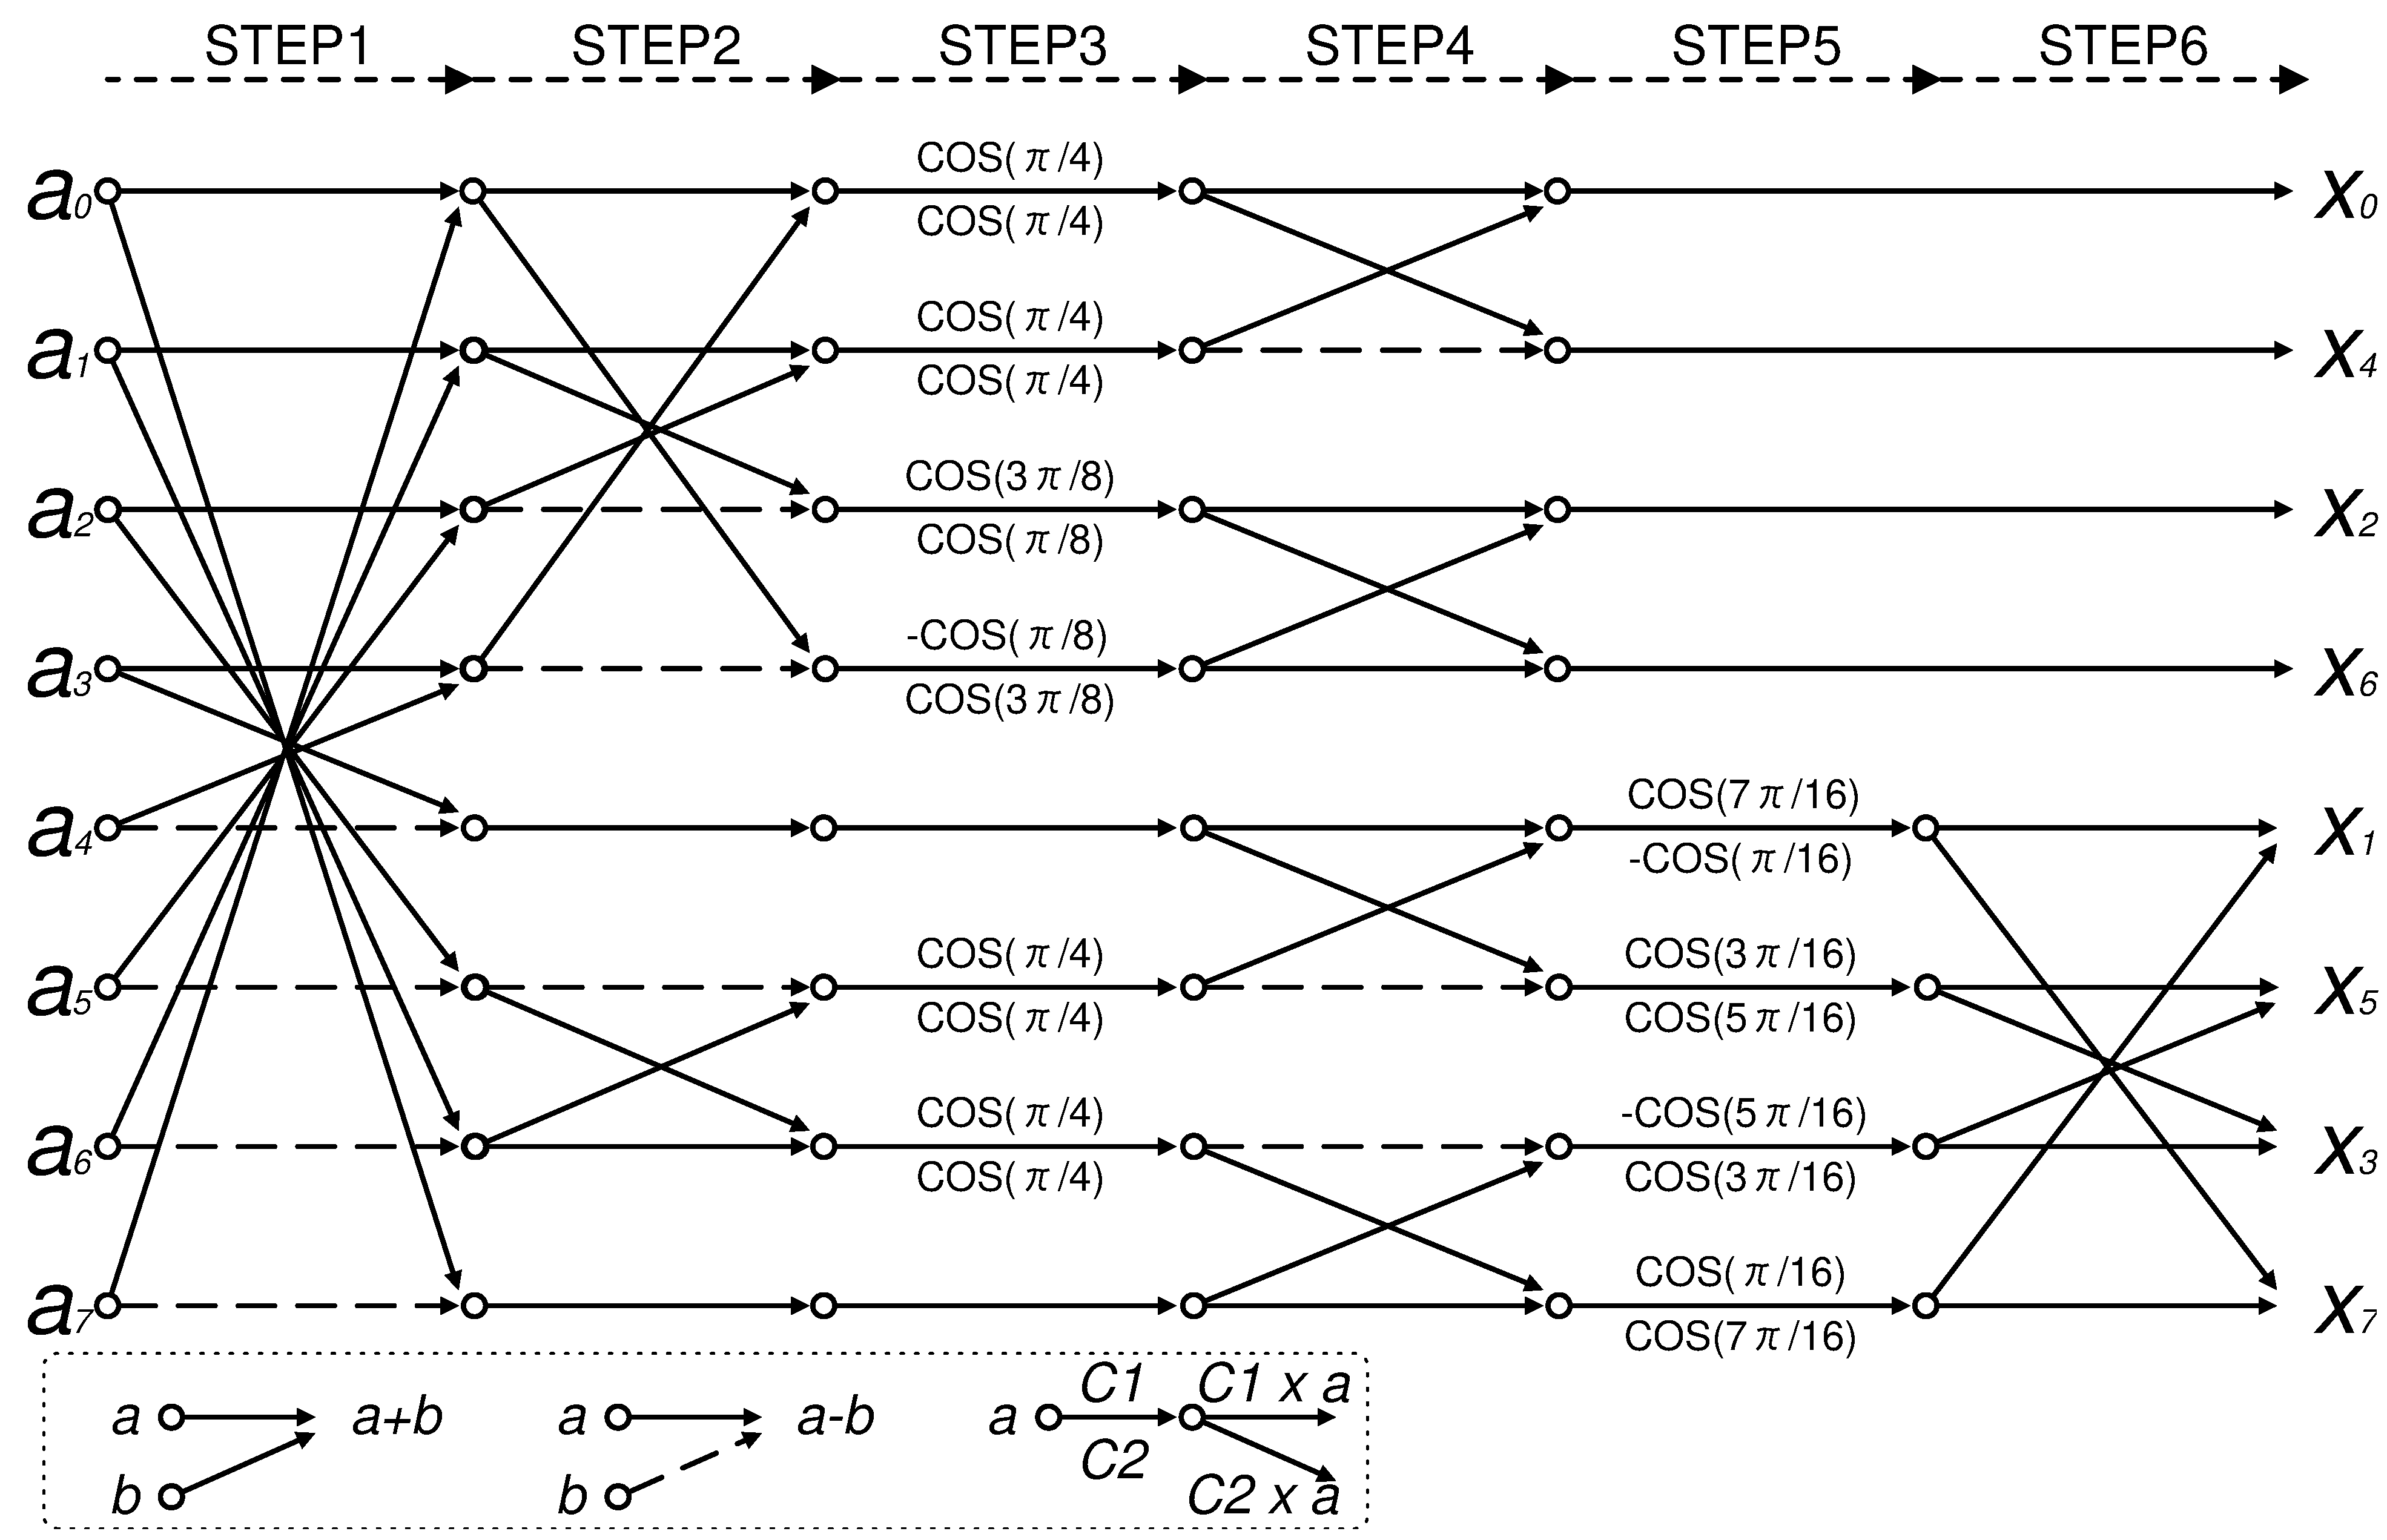
\includegraphics[width = 14cm,  height = 14cm, keepaspectratio, clip]{./pics/dct_flw.eps}
		\end{center}
		\caption{CAMベース超並列SIMD型プロセッサによる,高速DCTデータフロー.}
%		\ecaption{FMCAM with $d$ bits $\times$ $2^a$ words.}
		\label{dct_flw}
	\end{figure}%	
%figure	

%figure
	\begin{figure}[tbh]
		\begin{center}
			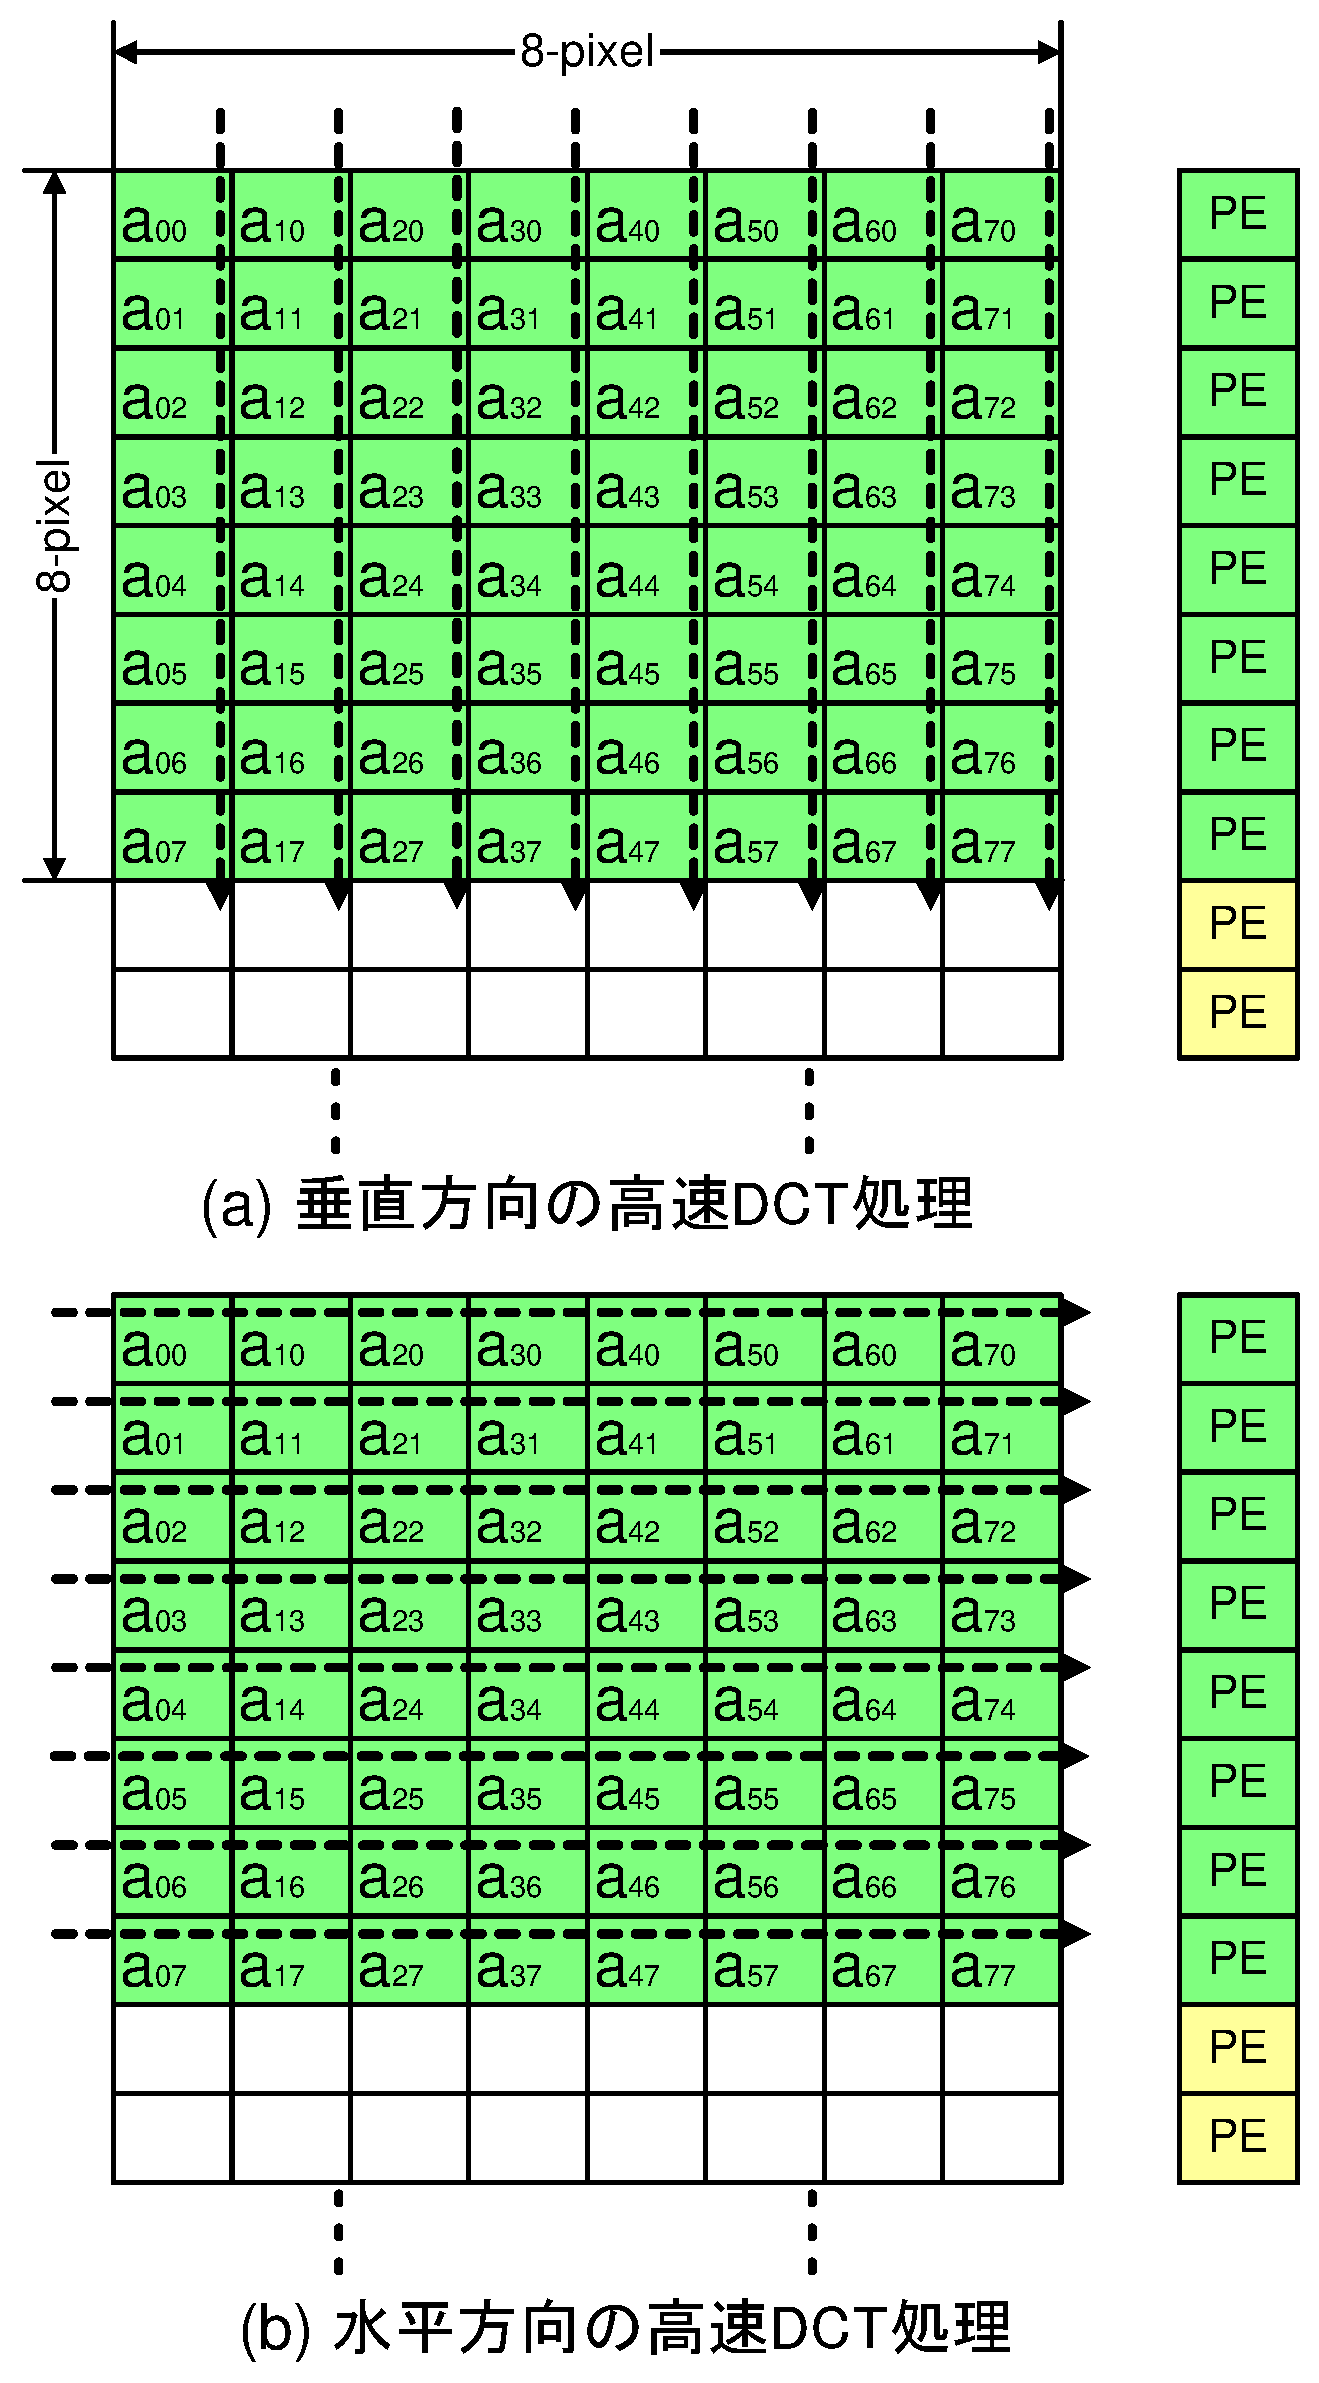
\includegraphics[width = 14cm,  height = 14cm, keepaspectratio, clip]{./pics/str_img.eps}
		\end{center}
		\caption{CAMベース超並列SIMD型プロセッサによる,高速DCT処理手法.}
%		\ecaption{FMCAM with $d$ bits $\times$ $2^a$ words.}
		\label{str_img}
	\end{figure}%	
%figure	



\item 並列処理の適用
	
		CAMベース超並列SIMD型プロセッサは,図 \ref{str_img}に示すように,
		N$_x$$ = $8,N$_y$$ = $8の画素の集合を,原画像の構成のままSRAMへ格納することが可能である.
		JPEGは,処理画像をN$_x$$ = $8,N$_y$$ = $8を1つの単位として,処理するため,
		一般のマルチメディアプロセッサは,図 \ref{dsp_simd}に示すようにデータを分割して処理する.
		これに対しCAMベース超並列SIMD型プロセッサは,垂直に配置することで,高い並列処理を実現することが可能である.
		CAMベース超並列SIMD型プロセッサの並列度が2,048である場合には,256並列に
		処理を行うことが可能である.

\item データ処理幅の変動に対する柔軟性
		
		DCT処理が行われるデータは,通常8 bitから始まる.
		このデータにコサインの乗算を繰り返すことで,データ長は,8 bit,16 bit,24 bit,32 bit,・・・
		と増加する.通常のマルチメディアデータ処理プロセッサは,図 \ref{dsp_simd}に示すような
		並列処理の手法をとっているため,データ長の変動は直接並列度の低下を招くこととなる.
		しかしながら,超並列SIMD型プロセッサの構成は,水平方向に256 bit以上と十分な長さを備えており,
		データの処理方向がビットシリアルであるため並列度の低下は無い.

\end{enumerate}

以上の検討より,CAMベース超並列SIMD型プロセッサによるDCT処理を詳述する.

\subsubsection{垂直方向高速DCT処理}
\label{lbl_cp5_jpg_dct_v}

CAMベース超並列SIMD型プロセッサによる,垂直方向高速DCT処理の流れを述べる.
高速DCT処理は,図 \ref{str_img}-(a)に示すデータフローによって行われ,
この処理を8回 (8画素列分)行う.
ここでは,図 \ref{dct_flw}に示すデータフロー中のSTEP2及びSTEP3について
図 \ref{mtx_flw}を用いて説明する.

STEP2は,2種類のバタフライ演算
によって処理される.
上方への移動を正,下方への移動を負とすると
各画素 (a$_0$,a$_1$,・・・,a$_7$)の移動度は,$\pm1$移動,$\pm3$移動から構成される.
前述したように垂直チャネルの移動量は2の累乗であるから,SIMD型アーキテクチャを
生かすために,この移動量をうまく組み合わせて共通に移動するデータを多くすることで
処理回数を削減できる.
例えばa$_0$の場合には,バリッドフラグを用いてマスク処理を行い,始めに$-$4移動
する.その後は$+$1移動が共通であるa$_0$,a$_2$及びa$_6$を移動し,減算することによって
a$_0$$ - $a$_3$,a$_6$$ - $a$_5$を同時に処理している.
STEP3では,乗算が主体となるので,データの移動後,各エントリにコサイン値を一斉に乗じることによって
処理の共通化を図っている.
なお,コサインの定数値やテンポラリの領域はポインタの指定で任意に扱うことが可能である.

%figure
	\begin{figure}[tbh]
		\begin{center}
			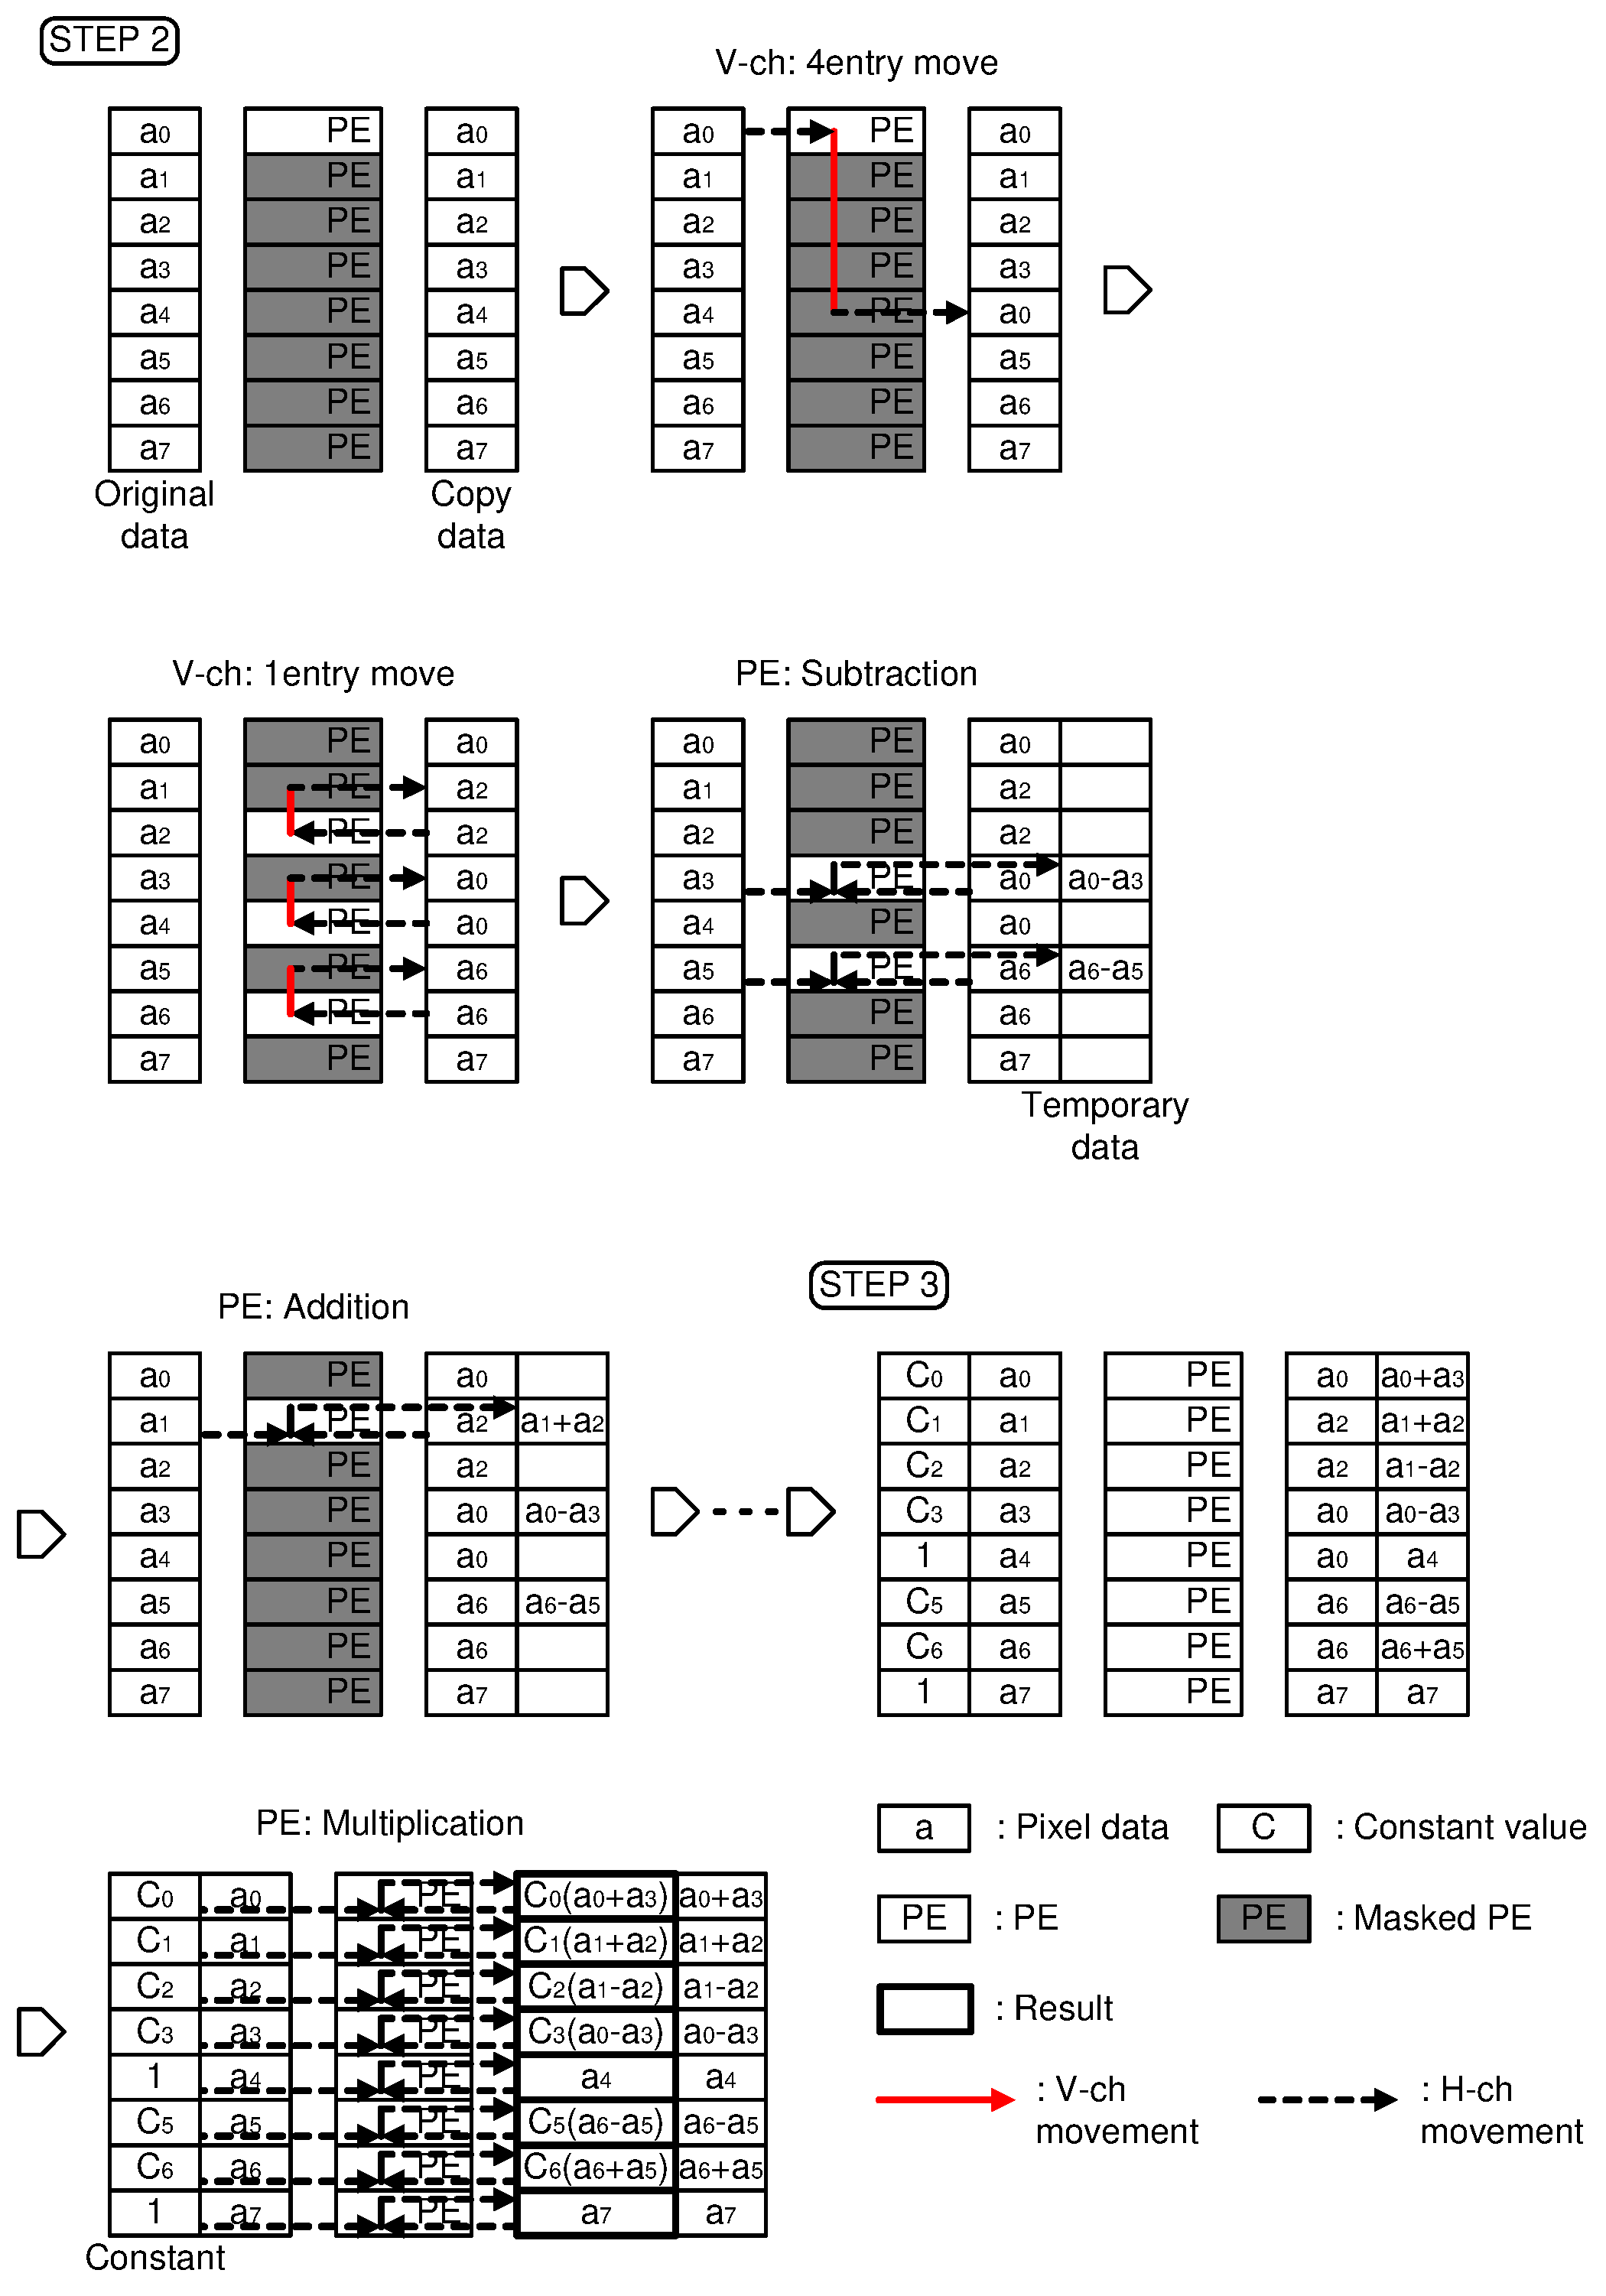
\includegraphics[width = 14cm,  height = 14cm, keepaspectratio, clip]{./pics/mtx_flw.eps}
		\end{center}
		\caption{CAMベース超並列SIMD型プロセッサによる垂直方向高速DCT処理.}
%		\ecaption{FMCAM with $d$ bits $\times$ $2^a$ words.}
		\label{mtx_flw}
	\end{figure}%	
%figure

\subsubsection{水平方向高速DCT処理}
\label{lbl_cp5_jpg_dct_h}

CAMベース超並列SIMD型プロセッサによる,水平方向高速DCT処理の流れを述べる.
水平方向の処理は,前述した垂直方向高速DCT処理後のデータに対して
行われる.高速DCT処理は,図 \ref{str_img}-(b)に示すデータフローによって行われる.
なお,水平方向の処理では全画素行に対しデータの全並列に処理を行うことができるので
データフローは1回のみ行えばよい.
ここでは,データフロー中のSTEP4及びSTEP5について図 \ref{mtx_sflw}を用いて説明する.

STEP4は,1種類のバタフライ演算が各エントリで行われる.水平方向の処理は水平チャネルのみ用いるため,移動度の制限は無い.
そのためデータフローで示されている,加算もしくは減算を順次行うだけでよい.
例では.STEP4-2で,a$_0$とa$_1$の加算を行い,STEP4-3でa$_0$とa$_1$の減算を行っている.
なお,必要に応じてテンポラリの領域を使用する.
STEP5に関しても,STEP4と同様に水平チャネルのみを行い,別領域に格納されているコサイン値と乗算を行うことで
実現可能である.


%figure
	\begin{figure}[tbh]
		\begin{center}
			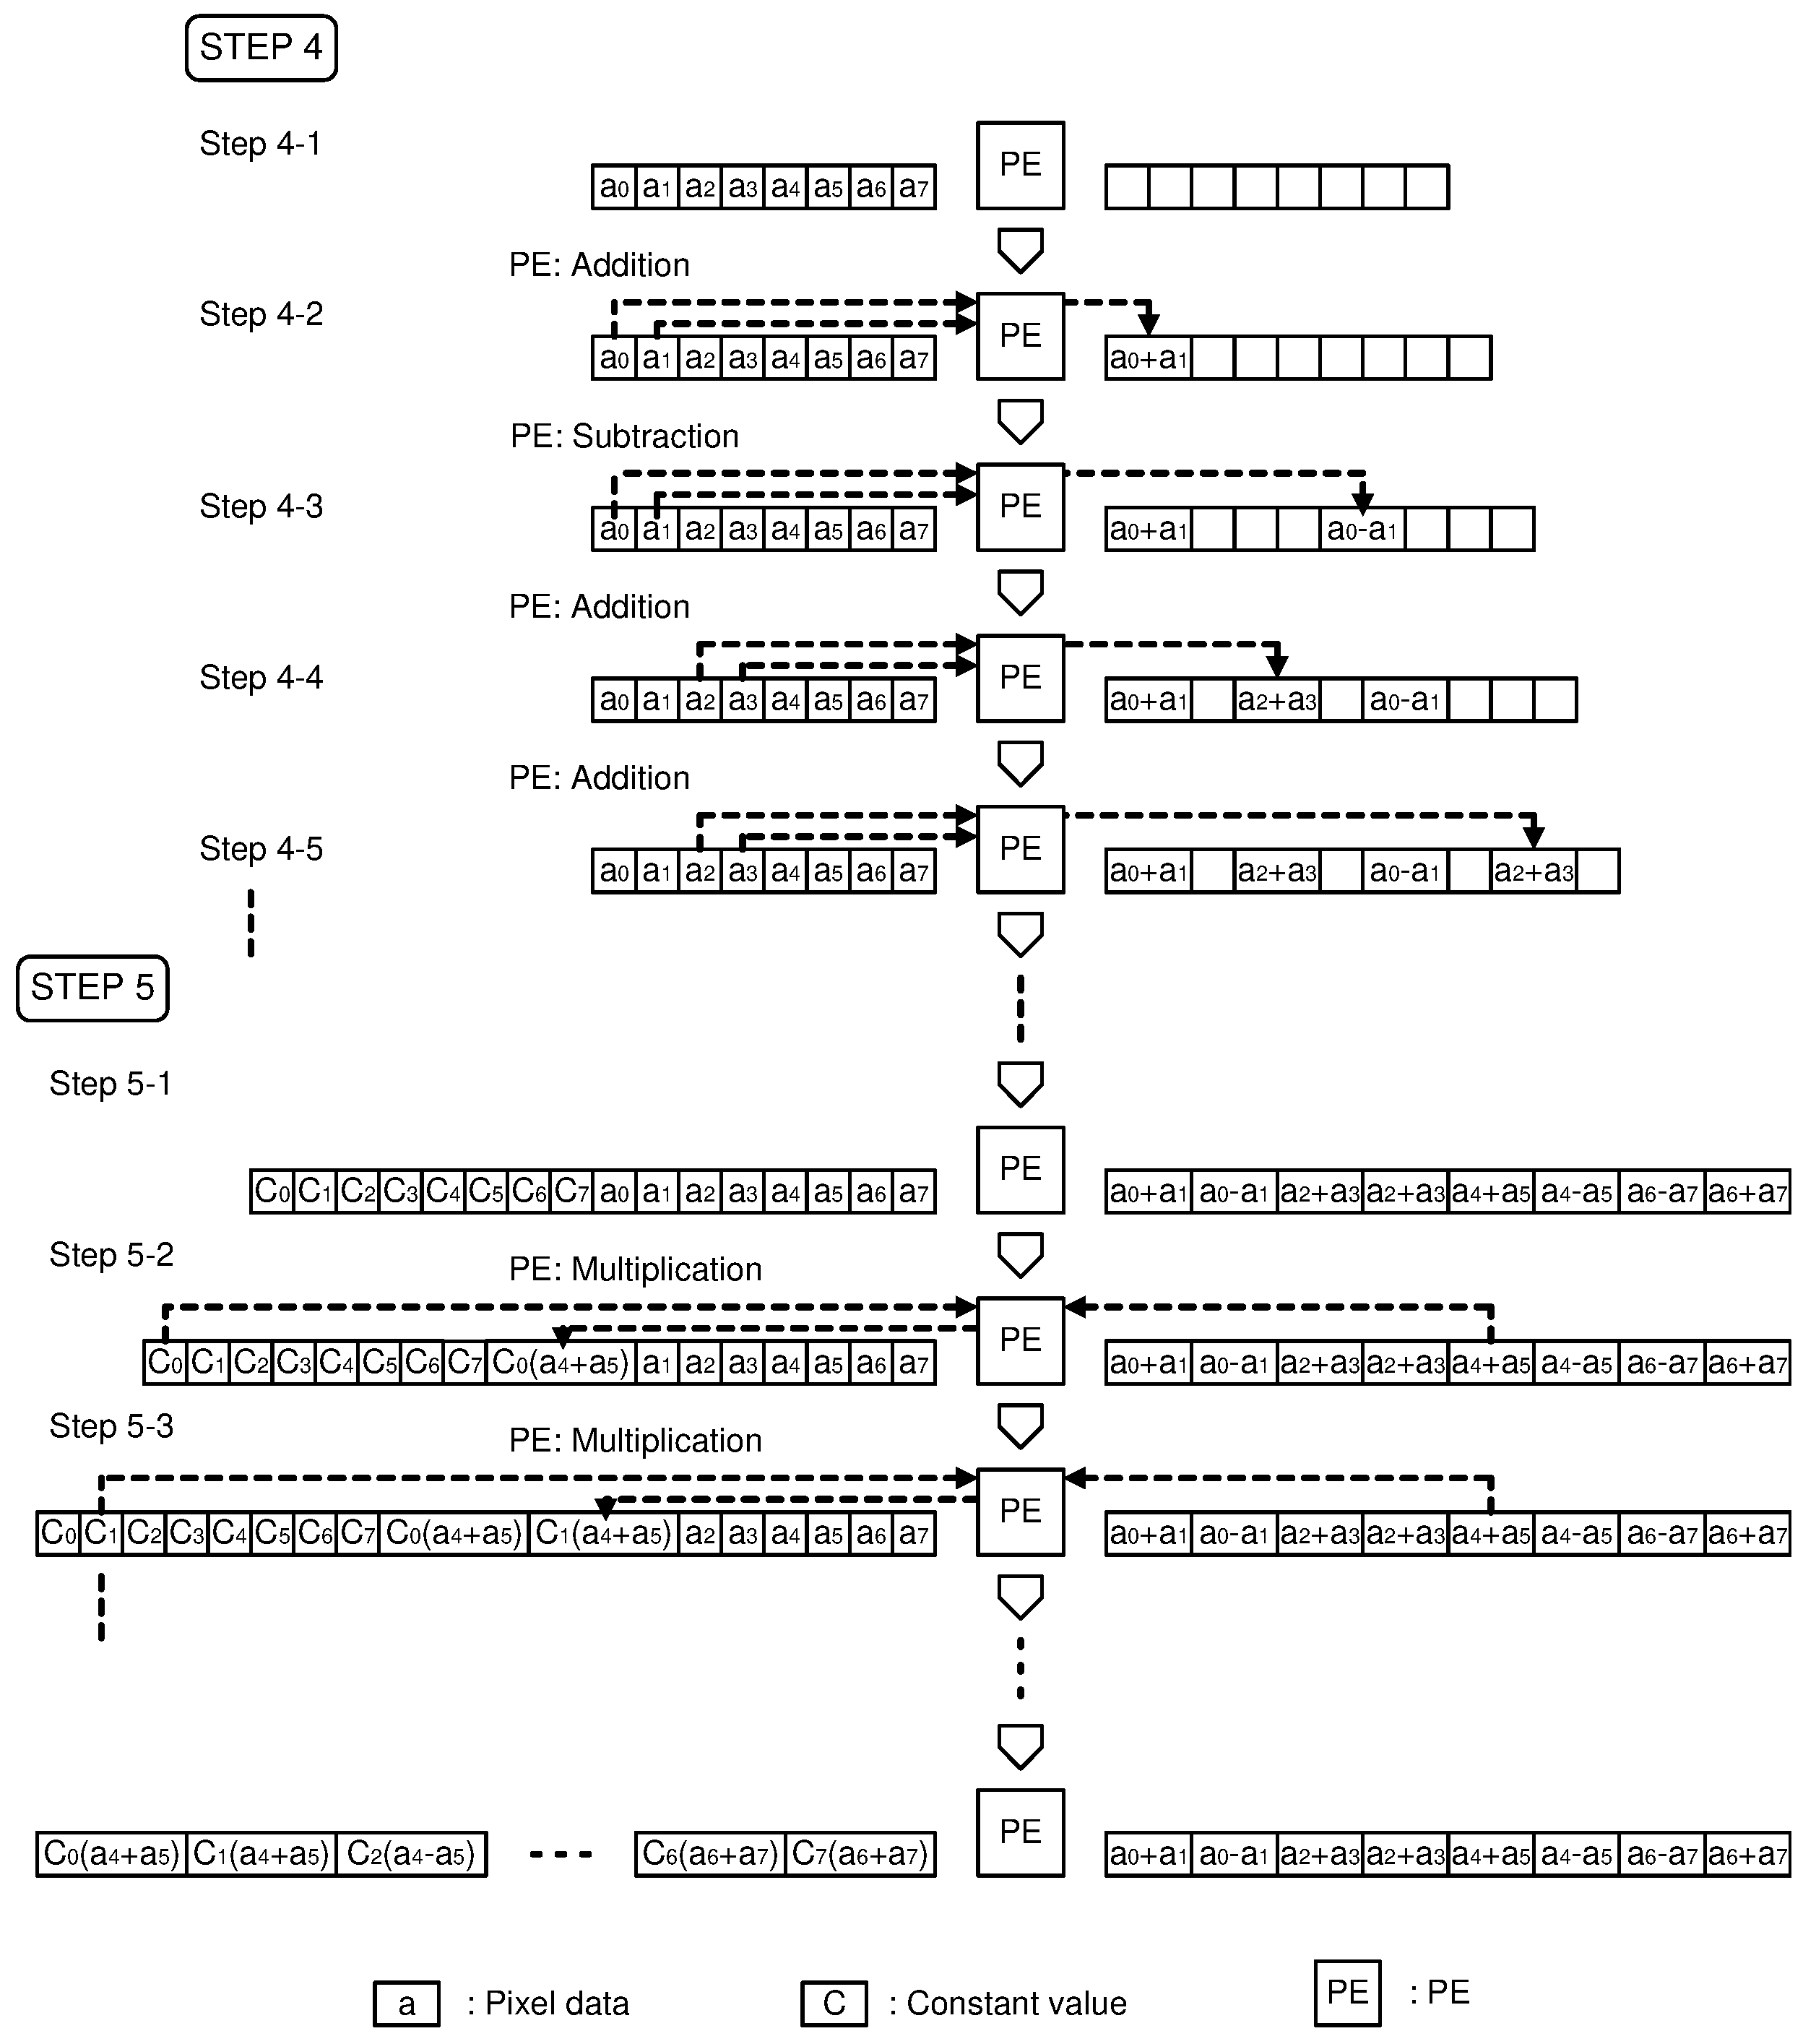
\includegraphics[width = 14cm,  height = 14cm, keepaspectratio, clip]{./pics/mtx_sflw.eps}
		\end{center}
		\caption{CAMベース超並列SIMD型プロセッサによる水平方向高速DCT処理.}
%		\ecaption{FMCAM with $d$ bits $\times$ $2^a$ words.}
		\label{mtx_sflw}
	\end{figure}%	
%figure



\subsubsection{DCT処理の評価}
\label{lbl_cp5_jpg_dct_hyoka}

CAMベース超並列SIMD型プロセッサによる,DCT処理の性能評価について述べる.
DCTは,コサインの乗算によってデータ長が変化するため,性能評価には
512 word $\times$ 1,024 entryのSRAMを2面用意して評価を行う.
%この構成に変更しても,\ref{lbl_cp5_mta_arch}で示した構成と比較して,メモリ領域の
%総サイズは1Mビットである.
比較対象のプロセッサは,90 nm CMOSテクノロジで製作された,
2命令同時発行VLIW (Very Long Instruction Word)アーキテクチャ16 bitのDSP
\cite{symdrp98, tmtmdv00, yyhskd00}
を選択した.動作周波数はどちらも200 MHzである.
図 \ref{dct_clk}に処理クロックサイクル数のグラフを示す.
横軸は処理クロック数である.
処理画像の総数は,1,024 entryに対して高速DCTにおける1つのブロックが,N$_y$$ = $8
ピクセルであることから,128ブロックとしている.
なお,画像の解像度の変化に伴い,CAMベース超並列SIMD型プロセッサ,及びDSP共に,
総クロックサイクル数は線形で増加する.
グラフより,CAMベース超並列SIMD型プロセッサは,DSPと比べて
クロックサイクル数を約87\%削減することが示せた.
この結果を元に,スループット (MOPS: Mega Operation Per Second)と実装面積で単位面積当たりの処理能力を評価する.
表 \ref{dct_mops}に算出結果を示す.
両アーキテクチャとも200 MHzで動作することから,スループットは約8倍の性能向上となった.
また,単位面積あたりの処理能力に関しても,5.6倍となった.

%figure
	\begin{figure}[tbh]
		\begin{center}
			\includegraphics[width = 12cm,  height = 12cm, keepaspectratio, clip]{./pics/dct_clk.eps}
		\end{center}
		\caption{CAMベース超並列SIMD型プロセッサ及びDSPによるJPEG処理クロックサイクル数の比較.}
%		\ecaption{FMCAM with $d$ bits $\times$ $2^a$ words.}
		\label{dct_clk}
	\end{figure}%	
%figure

%figure*
	\begin{table}[thb]
	\centering
		\begin{center}
		\caption{単位面積当たりの処理性能の比較.}
%			\includegraphics[width = 8.5cm, height = 8.5cm, keepaspectratio, clip]{impl_rslt.eps}
			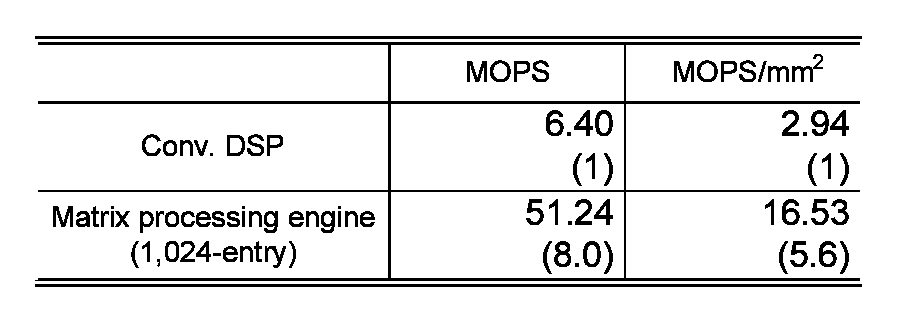
\includegraphics[width = 12cm, height = 12cm, keepaspectratio, clip]{./pics/dct_mops.eps}
		\label{dct_mops}
		\end{center}
	\end{table}%
%figure*

スループットの算出結果に関しては,CAMベース超並列SIMD型プロセッサが128並列に画像ブロックを高速DCTにて
処理できることから差がついたものと考えられる.
単位面積辺りの処理能力に関しては,SIMD型演算モジュールがSRAMデータレジスタバンクと演算器を密結合していること,
及び集積度の高いメモリをベースにしていることに起因していると考えられる.

\clearpage

\subsection{ハフマン符号化}
\label{lbl_cp5_jpg_huf}

この節では,CAMベース超並列SIMD型プロセッサによるハフマン符号化について述べる.
ハフマン符号化は図 \ref{baseline}に示した通り,ランレングス処理を経た,符号化前データが
ハフマンコードへ変換されることでデータ長が圧縮されるアルゴリズムである (アルゴリズムの詳細は,\ref{lbl_cp3_realtime_huffman}節を参照).
この処理は,JPEG方式の最後の処理であり,全体の処理の30\%を占めている\cite{pjpmik04, jorpje}.
従って,このアルゴリズムを高速に処理することは画像処理全体の処理時間を
大きく縮めることに直結し,マルチメディア処理LSIのパフォーマンスを大きく左右する.

CAMベース超並列SIMD型プロセッサは,\ref{lbl_cp5_mta_proc_huff}節に示した,
CAMを用いた高速なテーブルルックアップパイプライン処理によって,高速処理を実現できる.

\subsubsection{テーブルルックアップインターフェースによるハフマン符号化}
\label{lbl_cp5_jpg_huf_flw}
テーブルルックアップインターフェースは,直交SRAM,及びCAMを用いて
プログラマブルにデータの処理が行えるようなコントローラを有している.
図 \ref{huf_flw}に,テーブルルックアップインターフェースによる
ハフマン符号化のフローチャートを示し,その概要を説明する.
フローチャート前半の流れは,始めにコンフィギュレーションレジスタを``1"へセットすることにより,
CPUからのデータ入力に対してスルーモードへ設定することから始まる.
その後,CPUから,アドレス及びデータを逐次的に入力し,
CAMバンク0に符号化前データの全パターンを,CAMバンク1にハフマンコードテーブルを格納する.
ここまでが,符号化のための準備となる.
次に,コンフィギュレーションレジスタを``0"へセットした後に,バースト書込みのアドレスを指定して,
SIMD型演算モジュールへ,圧縮対象となる画像データを書き込む.
SIMD型演算モジュールのエントリ分画像データを格納したならば,
SIMD型演算モジュール内で,図 \ref{baseline}に示した,R,G及びBから,Y,C${_b}$及びC${_r}$への変換処理からランレングス処理まで
繰り返し演算処理を行う.
その後,SIMD型演算モジュール内の符号化前データを読み出しつつ,
ユーザプログラムを命令メモリから読み出し,直交SRAM,及びCAMを制御して,
\ref{lbl_cp5_mta_proc_huff}節にて述べた処理によりハフマン符号化を実行する.
CAMベース超並列SIMD型プロセッサは,CAMにハフマンコードテーブルを格納した後の処理を,
1,024,もしくは2,048 entry単位で実行でき,これを画素数分行うことで,JPEG処理が完了する.


%figure
	\begin{figure}[tbh]
		\begin{center}
			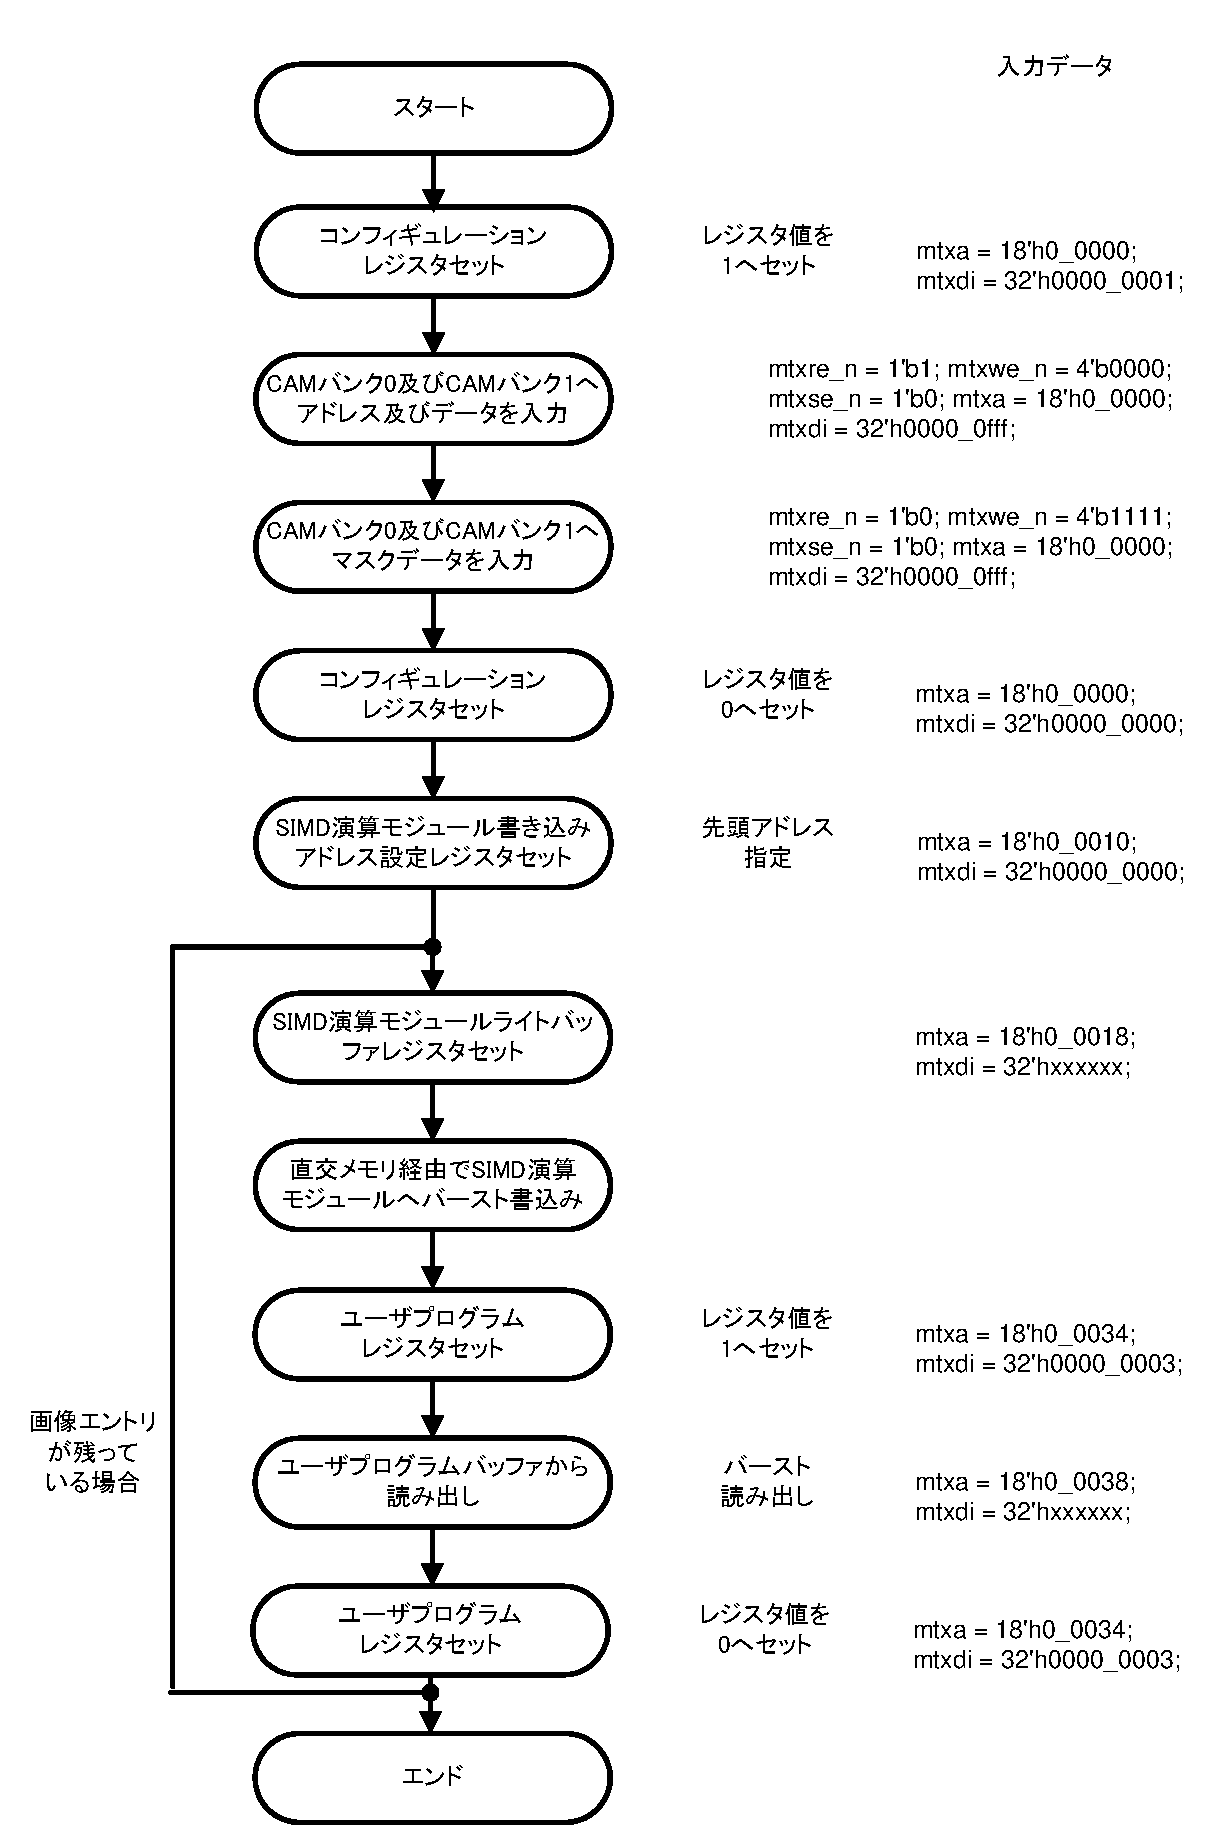
\includegraphics[width = 14cm,  height = 14cm, keepaspectratio, clip]{./pics/huf_flw.eps}
		\end{center}
		\caption{CAMベース超並列SIMD型プロセッサによるハフマン符号化処理.}
%		\ecaption{FMCAM with $d$ bits $\times$ $2^a$ words.}
		\label{huf_flw}
	\end{figure}%	
%figure

\subsubsection{信頼性評価}
\label{lbl_cp5_jpg_huf_flw}

テーブルルックアップインタフェースモジュールの開発については,
\ref{lbl_cp5_impl}節にて述べた.
このモジュールは,ユーザが作成したプログラムを,コントローラ内の命令メモリ
に格納し,SIMD型演算部からのデータをコントローラ,直交SRAM及びCAM
によって処理する.
そのため,性能を評価する前に,正確に各モジュールが協調動作しているかどうかの信頼性を検証する必要がある.
ここでは,テーブルルックアップインタフェースモジュールにて処理したデータと,
あらかじめソフトウェアで処理したデータを比較することにより,
アーキテクチャの信頼性を検証する.
信頼性の検証はテーブルルックアップインターフェースと,SIMD型演算モジュールのデータレジスタバンクを用意して行った.

検証環境は,Xilinx社のISE Foundation 7.1iを用いて論理合成及び配置配線し,
Mentor Graphics社のModelSimSE 5.8Cを使用してタイミング (遅延)シミュレーションを行った.
タイミングシミュレーションにてハフマン符号化処理を実施することにより,
ハードウェア実装時の遅延を考慮した環境を模擬した.
処理対象画像は結果が偏るのを防ぐため,サンプルデータは,カラー,モノクロ,人物,動物,及び背景等,様々な被写体を
選択した.サンプルデータを図 \ref{smp_pics0},図 \ref{smp_pics1},図 \ref{smp_pics2},図 \ref{smp_pics3},図 \ref{smp_pics4}
に示す.
これらは,192 $\times$ 128から,1,500 $\times$ 1,125までの解像度である画像25枚から構成される.
次に,信頼性検証の手順を図 \ref{ck_proc}に,その説明を以下に示す.

\begin{enumerate}
\item[{\ding{"C0}}] 検証用ビットマップ画像を,2,048 entry単位に分割し,
			テーブルルックアップインタフェースモジュールに入力.

\item[{\ding{"C1}}] テーブルルックアップインタフェースモジュール内で直交SRAMが,インターリーブ動作をしながら
			連続してSMID型演算モジュールへデータを転送.

\item[{\ding{"C2}}] SIMD型演算モジュール全エントリにデータが入力されたならば,
			再びテーブルルックアップインタフェースモジュールにデータを送信する (本来は,この間にハフマン符号化以外の処理が行われる).

\item[{\ding{"C3}}] 直交SRAMがインターリーブ動作をしつつ,CAMにデータを送信.
			CAMによりテーブルルックアップ動作が行われ,ハフマンコードが生成される.

\item[{\ding{"C4}}] ハフマンコードが符号後データとして,CAMベース超並列SIMD型プロセッサより出力され
			テキストデータとして保存される.

\item[{\ding{"C5}}] あらかじめ用意していた,ソフトウェアの結果と比較する.
\end{enumerate}

全ての画像についてデータの整合性を確認した結果,一致率は100\%となり,テーブルルックアップインターフェースアーキテクチャの
信頼性が確認できた.

また,この検証と共に処理クロックサイクル数の測定も行ったが,
この評価を含めた処理性能の評価は,\ref{lbl_cp5_jpg_hyoka}節にて,JPEGに含まれる他のアルゴリズムとあわせて行うことにする.


%figure
	\begin{figure}[tbh]
		\begin{center}
			\includegraphics[width = 11cm,  height = 11cm, keepaspectratio, clip]{./pics/smp_pics0.eps}
		\end{center}
		\caption{192 $\times$ 128,480 $\times$ 600及び512 $\times$ 480の検証用画像.}
%		\ecaption{FMCAM with $d$ bits $\times$ $2^a$ words.}
		\label{smp_pics0}
	\end{figure}%	
%figure

%figure
	\begin{figure}[tbh]
		\begin{center}
			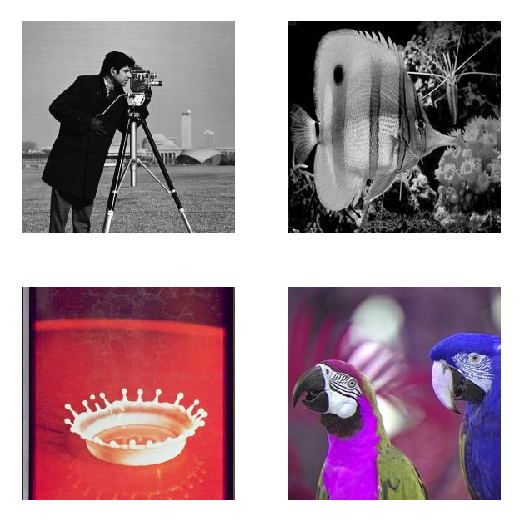
\includegraphics[width = 11cm,  height = 11cm, keepaspectratio, clip]{./pics/smp_pics1.eps}
		\end{center}
		\caption{256 $\times$ 256の検証用画像.}
%		\ecaption{FMCAM with $d$ bits $\times$ $2^a$ words.}
		\label{smp_pics1}
	\end{figure}%	
%figure


%figure
	\begin{figure}[tbh]
		\begin{center}
			\includegraphics[width = 11cm,  height = 11cm, keepaspectratio, clip]{./pics/smp_pics2.eps}
		\end{center}
		\caption{512 $\times$ 512の検証用画像.}
%		\ecaption{FMCAM with $d$ bits $\times$ $2^a$ words.}
		\label{smp_pics2}
	\end{figure}%	
%figure

%figure
	\begin{figure}[tbh]
		\begin{center}
			\includegraphics[width = 11cm,  height = 11cm, keepaspectratio, clip]{./pics/smp_pics3.eps}
		\end{center}
		\caption{600 $\times$ 480の検証用画像.}
%		\ecaption{FMCAM with $d$ bits $\times$ $2^a$ words.}
		\label{smp_pics3}
	\end{figure}%	
%figure

%figure
	\begin{figure}[tbh]
		\begin{center}
			\includegraphics[width = 11cm,  height = 11cm, keepaspectratio, clip]{./pics/smp_pics4.eps}
		\end{center}
		\caption{720 $\times$ 576,1,024 $\times$ 768及び1,500 $\times$ 1,125の検証用画像.}
%		\ecaption{FMCAM with $d$ bits $\times$ $2^a$ words.}
		\label{smp_pics4}
	\end{figure}%	
%figure

\clearpage

%figure
	\begin{figure}[tbh]
		\begin{center}
			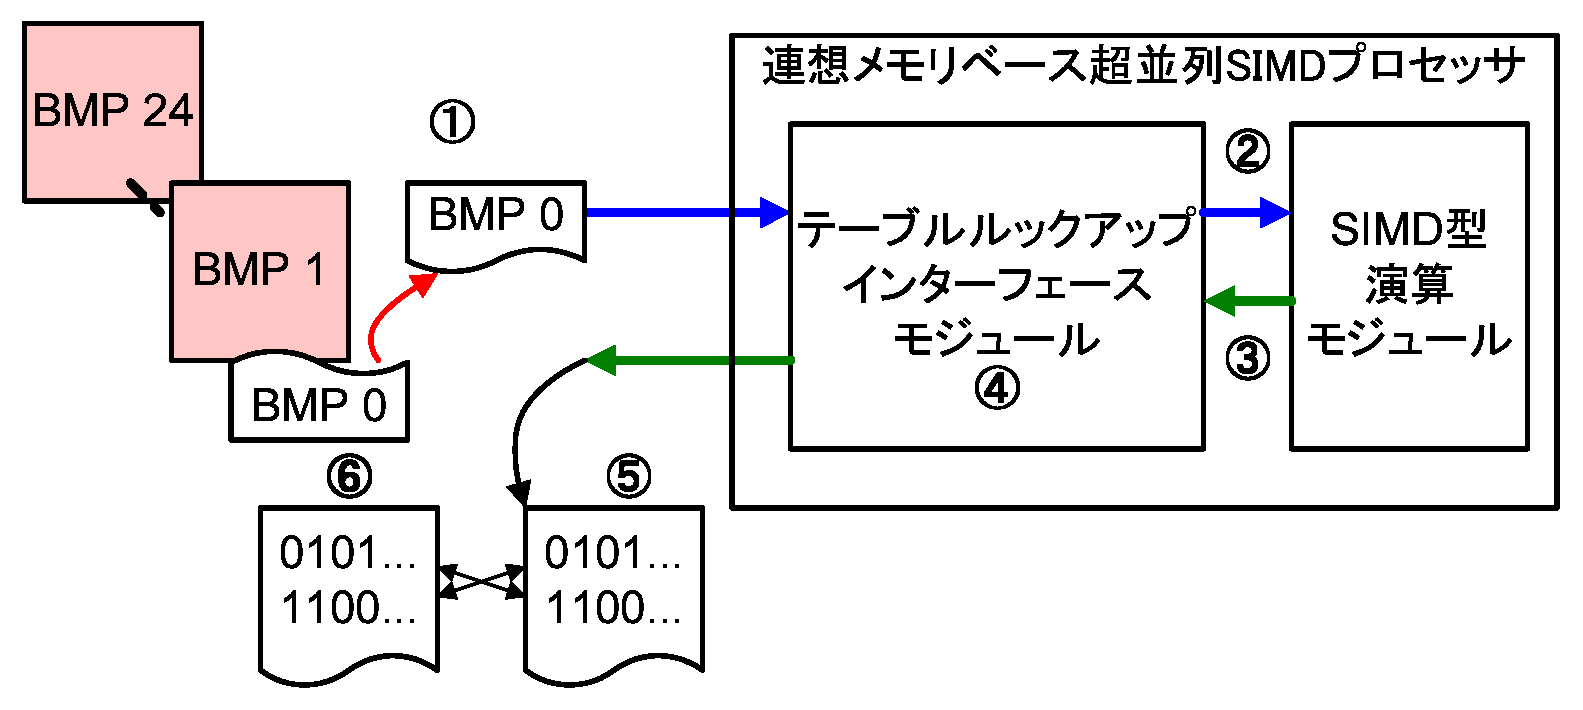
\includegraphics[width = 12cm,  height = 12cm, keepaspectratio, clip]{./pics/ck_proc.eps}
		\end{center}
		\caption{ハフマン符号化処理の信頼性検証手順.}
%		\ecaption{FMCAM with $d$ bits $\times$ $2^a$ words.}
		\label{ck_proc}
	\end{figure}%	
%figure




%\subsection{その他の処理}
%\label{lbl_cp5_jpg_etc}

%//後ほど書く

%\begin{itemize}
%\item RGBからYC$_b$C$_r$への変換,及びサンプリング

%カラー画像は,画素単位に色の三原色である,R (Red:赤),G (Green:緑),及びB (Blue:青)で表現することができる.
%しかしながら,人間の目は,色合いだけでなく明るさ (輝度)も感じ取ることができ,更には
%色合いより感度の幅が大きい.そこで,JPEGではRGBを輝度成分Y及び色差成分C$_b$及びC$_r$に分けることによって,
%人間の目に感度が高い輝度成分はそのままに,感度が低い色差成分をサンプリングによって削減する
%削減する手法をとる.

%RGBからYC$_b$C$_r$への変換式は以下の通りである.

%\begin{center}
%Y$ = $0.299R$ + $0.587G$ + $0.114B\\
%C$_b$$ = $0.713(R$ - $Y)$ + $128\\
%C$_r$$ = $0.564(R$ - $Y)$ + $128\\
%\end{center}


%\end{itemize}





\subsection{性能評価}
\label{lbl_cp5_jpg_hyoka}

この節では,%\ref{lbl_cp5_jpg_dct}節,及び\ref{lbl_cp5_jpg}節
%\ref{lbl_cp5_jpg_etc}節
%で述べた
CAMベース超並列SIMD型プロセッサによる各アルゴリズムの処理方法を元にして,
実画像を処理した結果を示す.また,その結果を元に既存のDSPと比較することで
性能評価を行う.

はじめに,ビットマップ画像からJPEG画像へと変換した際の,総処理クロック数について比較する.
対象画像は,\ref{lbl_cp5_jpg_huf_flw}にて検証用に用いたJPEG画像である.
比較対象アーキテクチャは,SRAMベース超並列SIMD型プロセッサと
一般的な2命令同時発行VLIW (Very Long Instruction Word)アーキテクチャである16 bit
のDSP\cite{symdrp98, tmtmdv00, yyhskd00}である.
処理にかかった総クロックサイクル数を表 \ref{jpg_tbl}に示す.
今回は,圧縮にオプションを指定しない通常のJPEGアルゴリズムを使用している.
また,R,G及びBからY,C$_b$及びC$_r$を
生成する際に,サンプリングを考慮しないようにするためY画像のみを取り扱った.
そのため,画像の視覚的特長が異なる場合でも,処理データ自体は異なるが,ピクセル数が同一であれば
クロックサイクル数は同じ値となる.
比較の結果,DSPはDCT処理やハフマン符号化において並列度が低く,
テーブルルックアップ処理が逐次的な処理のため,どの画像においても,最も大きい値となった.
SRAMベースの超並列SIMD型プロセッサは,DCT等の処理を高速に行えるため,DSPに比べて
処理クロックサイクル数は少ないことが分かった.
これらの結果に対して,
SRAMベースの超並列SIMD型プロセッサに,CAMベーステーブルルックアップ符号化アーキテクチャを
融合させたCAMベース超並列SIMD型プロセッサは,
DCT等の処理を超並列に処理しつつ,テーブルルックアップ処理も高速に行えるため,
最もクロックサイクル数が少なく,高速に処理を行えることが分かる.
ここで,図 \ref{jpg_clk}に,DCTとハフマン符号化,及びその他の処理の
クロックサイクル数を視覚的に表したグラフを示す.
なお,一般にランレングス処理後は,データの個数自体が減少するが,
超並列SIMD型アーキテクチャでエントリを削減するためには,垂直チャネルで
エントリを移動せねばならず,クロックサイクル数を消費することになる.
そのため,ブランクなエントリが存在するものとして,処理を行っているので,
各処理クロックサイクル数は総ピクセル数と比例関係にある.
また,DSPのクロックサイクル数に関しても8 $\times$ 8のピクセルブロックで
正規化した値を使用しているので,ピクセル数と比例関係にある.
従って,ここでは256 $\times$ 256サイズの画像を例として使用する.
表 \ref{jpg_tbl}の結果を元に,4:2:2のカラー画像のクロックサイクル数を
見積もった値を使用した.
横軸は,各アーキテクチャの名前,縦軸は処理クロックサイクル数である.
各グラフとも上からDCT,ハフマン符号化,及びその他の処理
の順でクロックサイクル数を分けている.
グラフから分かるように,SRAMベース超並列SIMD型アーキテクチャは並列度を増加させることで,
DSPと比較して総クロックサイクル数を約48\%削減している.
特にDCTに関しては,97\%もの削減を実現している.
しかしながら,並列度を向上させた代わりに,逐次処理が主体となる
ハフマン符号化のボトルネックが顕著に現れる結果となり,ハフマン符号化の
クロックサイクル数は約2.4倍となった.
CAMベース超並列SIMD型プロセッサは,インタフェースモジュールに
CAMを融合させることでテーブルルックアップ処理を高速に行うことが可能となったため,
SRAMベース超並列SIMD型プロセッサのボトルネックである,ハフマン符号化を
大幅に削減することに成功した.削減率は約92\%にまで達している.
また,DSPと比較しても74\%の削減となった.
総クロックサイクル数で比較すると,SRAMベースの超並列SIMD型プロセッサと比較して,
約73\%の削減を達成し,DSPとの比較では,約86\%の削減を実現した.

CAMベース超並列SIMD型プロセッサは,SRAMベース超並列SIMD型プロセッサの
インターフェース部にCAMやコントローラを融合させたアーキテクチャとなっている.
この構成をとることによって,クロックサイクル数の削減を実現できたが,
同時に面積も増加することになる.そこで面積を考慮した上での,
性能評価を表 \ref{jpg_ppa}に示す.
評価は,単位面積当たりの処理ピクセル数とした.
各アーキテクチャは全て200 MHzで動作する.
また,テーブルルックアップインタフェースモジュールの実装状況にあわせて,
(a)をソフトマクロ使用時,(b)をハードマクロ (直交SRAM,及びCAM)使用時とした.
表より,ソフトマクロ使用時では,CAMベース超並列SIMD型プロセッサは,CAMとコントローラの
面積増加にも関わらず,SRAMベースの場合と比較して,約3倍の
処理性能を持つことが分かった.
また,DSPとの比較では約4倍もの処理性能を持つことが分かった.
ハードマクロ使用時では,CAMベース超並列SIMD型アーキテクチャの値は6.20となり,
SRAMベースの場合と比較して,約3.3倍,DSPとの比較では約4.4倍になることが分かった.
なお,消費電力に関しても考察すると,
SIMD型演算モジュールが繰り返し演算を行っている間は,
テーブルルックアップインタフェースモジュールはデータを転送するのみである.
すなわちCAMによる一致検索処理は行わない.
また,反対にテーブルルックアップ処理を行っている際には,SIMD型演算モジュールで
演算処理は行われない.
そのため,CAMベース超並列SIMD型プロセッサの消費電力は,
SRAMベースと同様の250 mWであると見積もることができる.

以上の検証より,SRAMベースの超並列SIMD型プロセッサに,CAMベーステーブルルックアップ符号化アーキテクチャを
融合させたCAMベース超並列SIMD型プロセッサは,マルチメディアデータの繰り返し演算処理と
テーブルルックアップ処理を,どちらも効率的に処理できるアーキテクチャであることが分かった.
また,アーキテクチャの融合に伴う面積の増加率も,処理性能と比較した場合,
わずかなものであることが分かった.


%figure*
	\begin{table}[thb]
	\centering
		\begin{center}
		\caption{JPEG処理クロックサイクル数の比較 (Y画像).}
%			\includegraphics[width = 8.5cm, height = 8.5cm, keepaspectratio, clip]{impl_rslt.eps}
			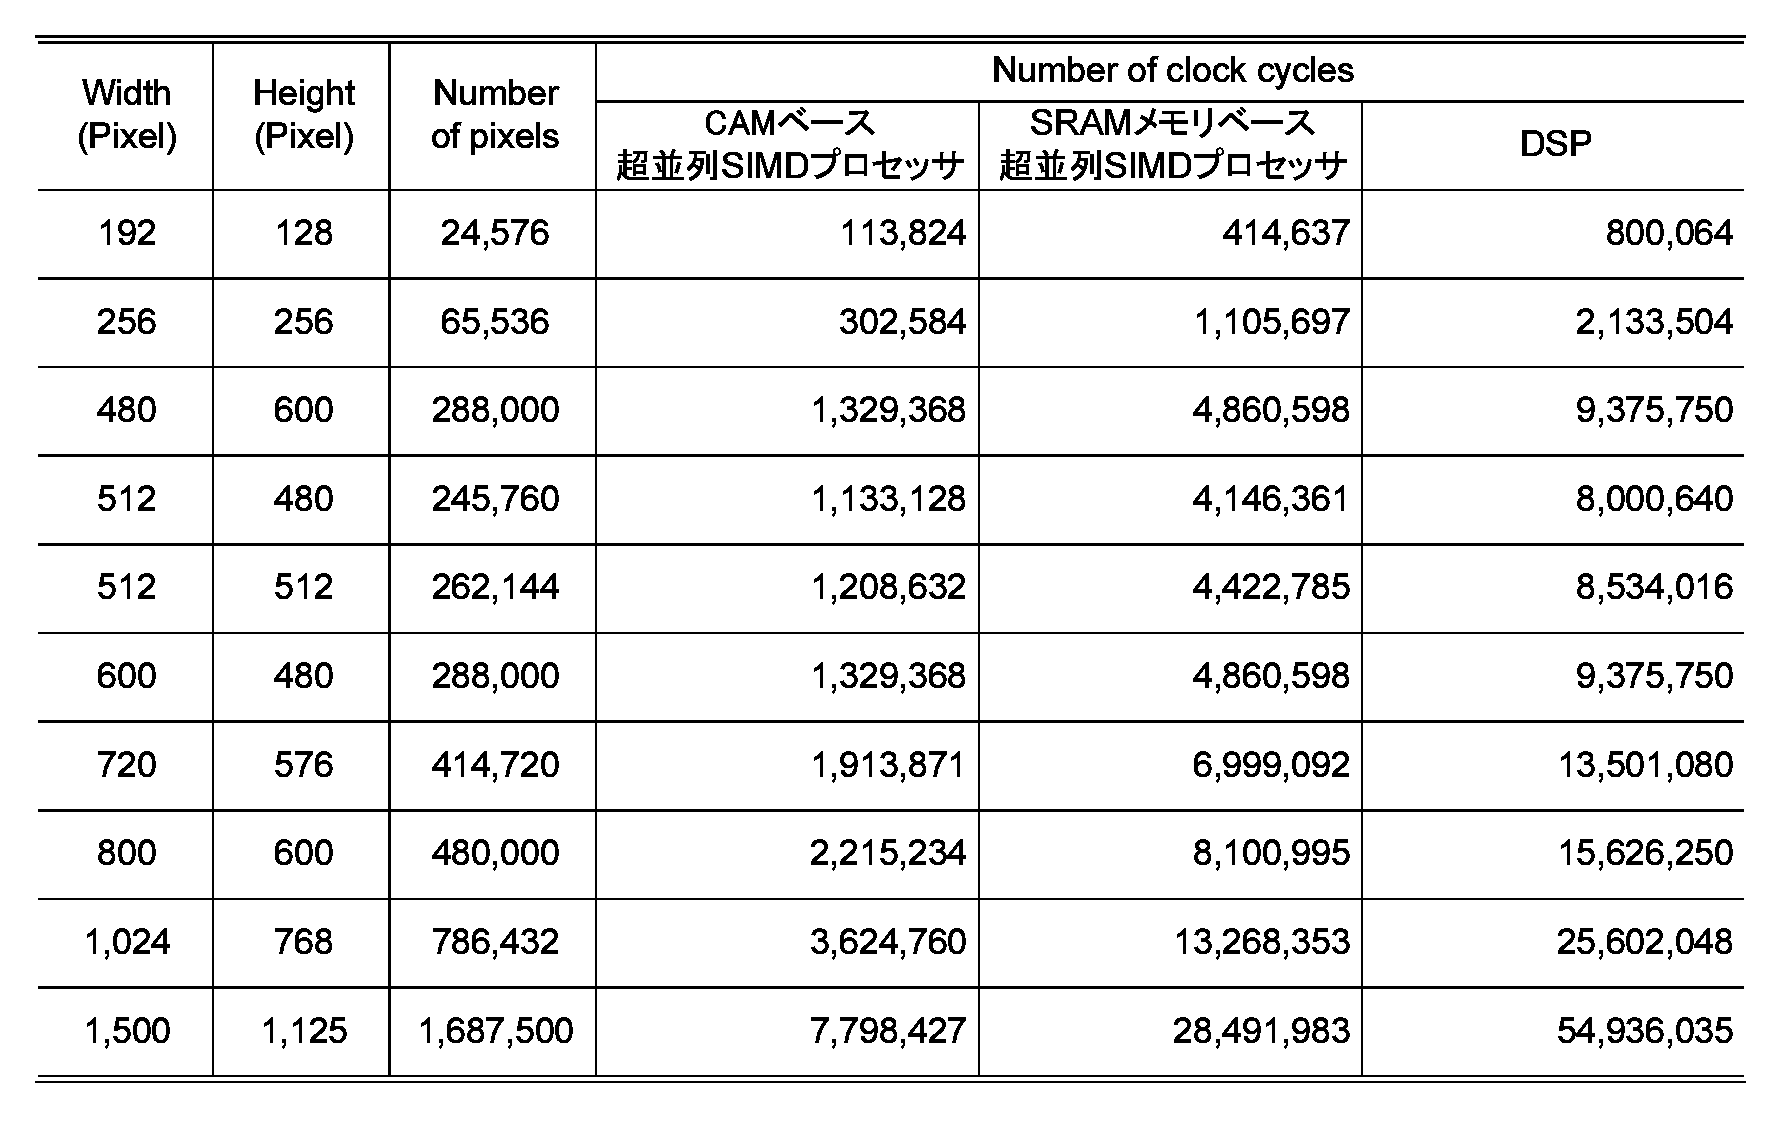
\includegraphics[width = 14cm, height = 14cm, keepaspectratio, clip]{./pics/jpg_tbl.eps}
		\label{jpg_tbl}
		\end{center}
	\end{table}%
%figure*

%figure
	\begin{figure}[tbh]
		\begin{center}
			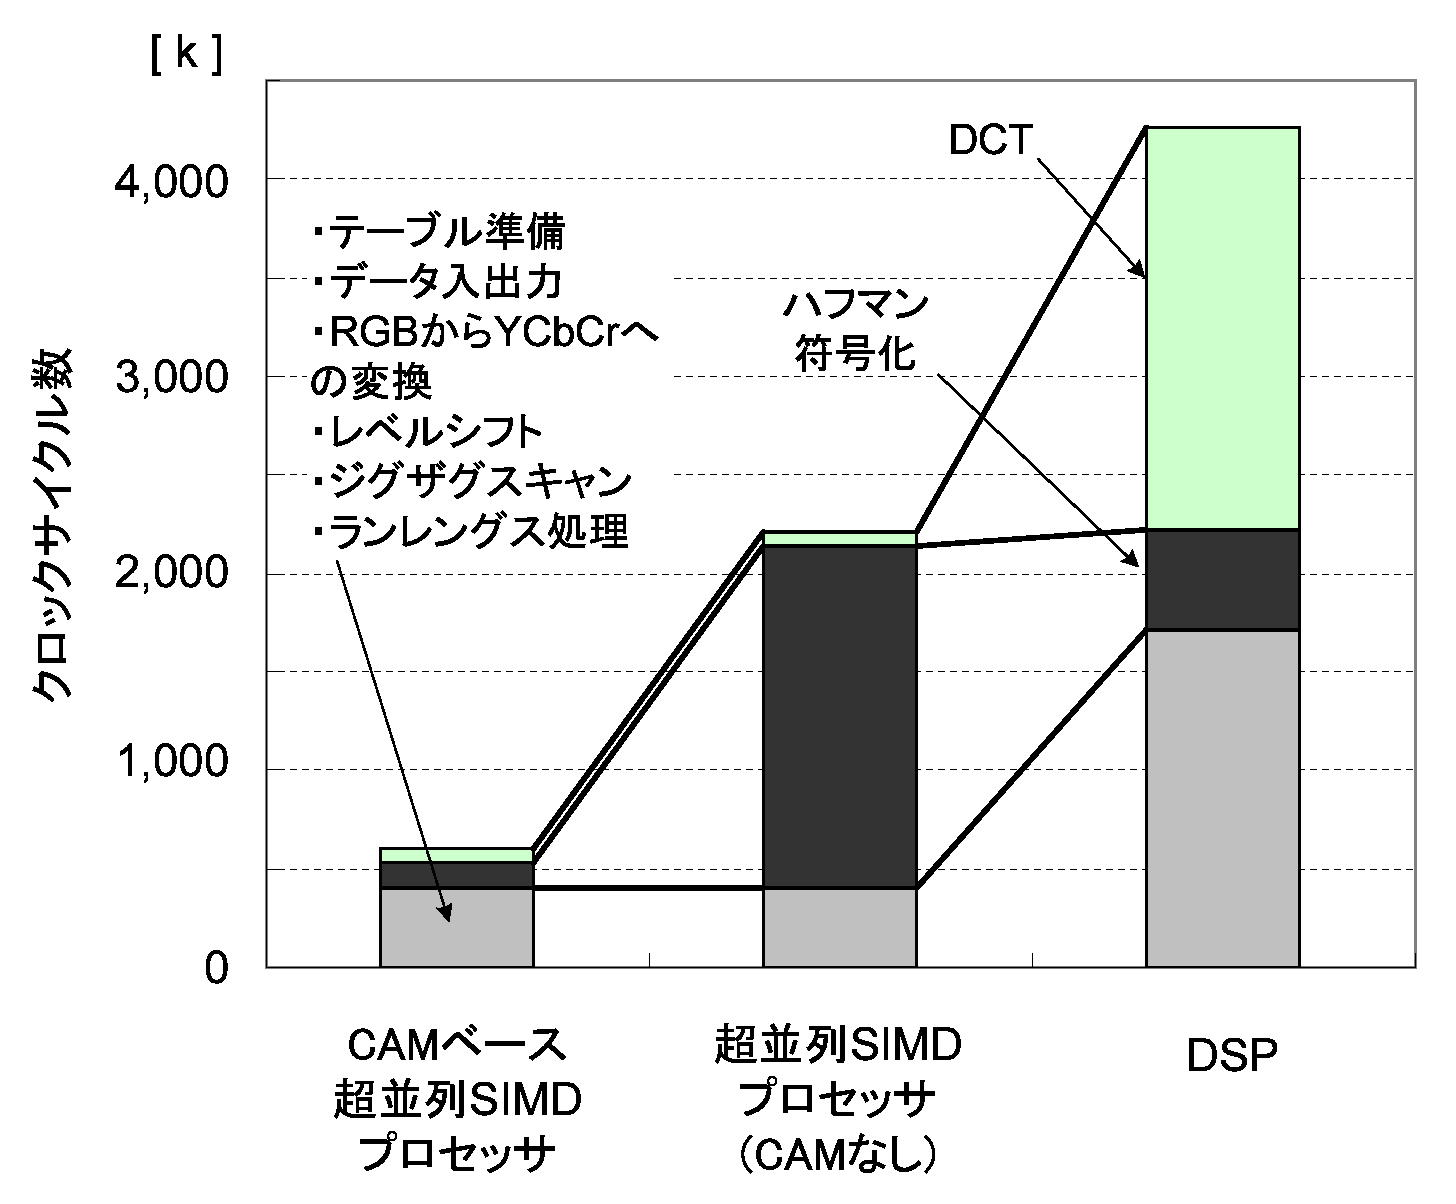
\includegraphics[width = 14cm,  height = 14cm, keepaspectratio, clip]{./pics/jpg_clk.eps}
		\end{center}
		\caption{各アーキテクチャによるクロックサイクル数の比較 (2,048 entry,Y,C$_b$,及びC$_r$画像).}
%		\ecaption{FMCAM with $d$ bits $\times$ $2^a$ words.}
		\label{jpg_clk}
	\end{figure}%	
%figure

%figure*
	\begin{table}[thb]
	\centering
		\begin{center}
		\caption{単位面積当たりの処理能力の比較.}
%			\includegraphics[width = 8.5cm, height = 8.5cm, keepaspectratio, clip]{impl_rslt.eps}
			\includegraphics[width = 14cm, height = 14cm, keepaspectratio, clip]{./pics/jpg_ppa.eps}
		\label{jpg_ppa}
		\end{center}
	\end{table}%
%figure*


%\section{暗号処理アルゴリズムへの適用}
%\label{lbl_cp5_ango}

%\section{階層並列構造SIMD型プロセッサアーキテクチャ}
%\label{lbl_cp5_ango}

\clearpage

\section{まとめ}
\label{lbl_cp5_matome}

本章では,テーブルルックアップ処理,及び繰り返し演算処理を
どちらも高速に処理することのできるCAMベースの新しいアーキテクチャを提案,開発した.
これはマルチメディア処理のボトルネックであるテーブルルックアップ符号化処理を高速に行うことを可能とし,
繰り返し演算処理を2,048並列のSIMD型プロセッシングユニットで行うことにより高速化を実現するアーキテクチャである.
提案アーキテクチャはCAM,SRAM,及びPEを融合した構造をとっているため小面積での高並列処理を実現し,
単位面積当たりの演算能力を上げることで,動作周波数を抑え,低消費電力化を実現している.
更に,CAMとSRAMアレイのデータ転送を工夫することにより,パイプライン処理も実現している.
従来のDSP等と比較した結果,JPEGアプリケーションにおいては,最大87\%のクロックサイクル数の削減を可能とし,
単位面積あたりの処理能力では,約4.4倍の能力を有することがわかった.
消費電力に関しても,モバイル用途向けに問題とならない程度であることを議論した.
%また,暗号処理アルゴリズムであるAESにおいては約15倍のスループットを達成した.

以上より,提案アーキテクチャは従来のマルチメディアデータ処理LSIでは実現が難しかった
テーブルルックアップ処理,及び繰り返し演算処理の効率的な両立を,アーキテクチャを工夫することで
可能とした.
また,マルチメディアデータ処理のみならず,プログラマブルに様々なアプリケーションに適用できる構成であることも
示した.
